\documentclass[notes,10pt, aspectratio=169]{beamer}

\usepackage{pgfpages}
% These slides also contain speaker notes. You can print just the slides,
% just the notes, or both, depending on the setting below. Comment out the want
% you want.
\setbeameroption{hide notes} % Only slide
%\setbeameroption{show only notes} % Only notes
%\setbeameroption{show notes on second screen=right} % Both
\usepackage{colortbl}
\usepackage{helvet}
\usepackage[default]{lato}
\usepackage{array}
\usepackage{eurosym}
\usepackage{setspace}
\usepackage{animate}
\usepackage{multicol}
\usepackage{breqn}
\usepackage{subcaption}
\usepackage{caption}
\captionsetup{font=scriptsize, justification=raggedright,singlelinecheck=false}
\usepackage[export]{adjustbox}
\usepackage[scale=2]{ccicons}
\usepackage{tikz}
\newenvironment{wideitemize}{\itemize\addtolength{\itemsep}{10pt}}{\enditemize}
\usepackage{natbib}

\usepackage{tikz}
\usepackage{verbatim}
\setbeamertemplate{note page}{\pagecolor{yellow!5}\insertnote}
\usepackage{amsmath}
%\usepackage{mathpazo}
\usepackage{hyperref}
\usepackage{lipsum}
\usepackage{multimedia}
\usepackage{multirow}
\usepackage{graphicx}
\usepackage{dcolumn}
\usepackage{bbm}
\newcolumntype{d}[0]{D{.}{.}{5}}

\usepackage{changepage}
\usepackage{appendixnumberbeamer}
% \newcommand{\beginbackup}{
%   \newcounter{framenumbervorappendix}
%   \setcounter{framenumbervorappendix}{\value{framenumber}}
%   \setbeamertemplate{footline}
%   {
%      \leavevmode%
%      \hline
%      box{%
%       \begin{beamercolorbox}[wd=\paperwidth,ht=2.25ex,dp=1ex,right]{footlinecolor}%
% %         \insertframenumber  \hspace*{2ex} 
%       \end{beamercolorbox}}%
%      \vskip0pt%
%   }
%  }

 \setbeamertemplate{footline}{
    \hbox{%
    \begin{beamercolorbox}[wd=\paperwidth,ht=3ex,dp=1.5ex,leftskip=2ex,rightskip=2ex]{page footer}%
        %\usebeamerfont{title in head/foot}%
        %\insertshorttitle \hfill
        %\insertsection \hfill
        %\tableofcontents[currentsection] \hfill
        \insertsectionnavigationhorizontal{0.7\paperwidth}{}{} \hfill 
        \insertframenumber{} / \inserttotalframenumber
    \end{beamercolorbox}}%
}
\newcommand{\backupend}{
   \addtocounter{framenumbervorappendix}{-\value{framenumber}}
   \addtocounter{framenumber}{\value{framenumbervorappendix}} 
}

\useinnertheme[shadow]{rounded}
\setbeamercolor{block title example}{fg=black,bg=orange!50!white}
\setbeamercolor{block body example}{fg=black, bg=orange!30!white}
\setbeamercolor{block title alert}{fg=black,bg=green!50!white}
\setbeamercolor{block body alert}{fg=black, bg=green!30!white}
\setbeamercolor{block title}{use=structure,fg=structure.fg,bg=structure.fg!20!bg}
\setbeamercolor{block body}{parent=normal text,use=block title,bg=block title.bg!50!bg}

\newcommand\independent{\protect\mathpalette{\protect\independenT}{\perp}}
\def\independenT#1#2{\mathrel{\rlap{$#1#2$}\mkern2mu{#1#2}}}

\usepackage{graphicx}
\usepackage[space]{grffile}
\usepackage{booktabs}

% These are my colors -- there are many like them, but these ones are mine.
\definecolor{blue}{RGB}{0,114,178}
\definecolor{red}{RGB}{213,94,0}
\definecolor{yellow}{RGB}{240,228,66}
\definecolor{green}{RGB}{0,158,115}

\setbeamercolor{section in head/foot}{fg=blue}


\hypersetup{
  colorlinks=false,
  linkbordercolor = {white},
  linkcolor = {blue}
}


%% I use a beige off white for my background
\definecolor{MyBackground}{RGB}{255,253,218}

%% Uncomment this if you want to change the background color to something else
%\setbeamercolor{background canvas}{bg=MyBackground}

%% Change the bg color to adjust your transition slide background color!
\newenvironment{transitionframe}{
  \setbeamercolor{background canvas}{bg=yellow}
  \begin{frame}}{
    \end{frame}
}

\setbeamercolor{frametitle}{fg=blue}
\setbeamercolor{title}{fg=black}
%\setbeamertemplate{footline}[frame number]
\setbeamertemplate{navigation symbols}{} 
\setbeamertemplate{itemize items}{-}
\setbeamercolor{itemize item}{fg=blue}
\setbeamercolor{itemize subitem}{fg=blue}
\setbeamercolor{enumerate item}{fg=blue}
\setbeamercolor{enumerate subitem}{fg=blue}
\setbeamercolor{button}{bg=white,fg=blue,}



% If you like Traffic maps, rather than having clutter at the top, have a Trafficmap show up at the end of each section 
% (and after your introduction)
% Uncomment this is if you want the Trafficmap!
% \AtBeginSection[]
% {
%    \begin{frame}
%        \frametitle{Trafficmap of Talk}
%        \tableofcontents[currentsection]
%    \end{frame}
% }
\setbeamercolor{section in toc}{fg=blue}
\setbeamercolor{subsection in toc}{fg=red}
%\setbeamersize{text margin left=1em,text margin right=1em} 
\setbeamersize{text margin left=0.7cm,text margin right=0.7cm} 


\title[]{\textcolor{blue}{Lecture 10:\\An Introduction to Panel Data}}
\author{25117 - Econometrics}
\institute[shortinst]{Universitat Pompeu Fabra}

\date{November 20th, 2024}

\begin{document}

\begin{frame}[plain]
\maketitle
\end{frame}



\begin{frame}{What we learned in the last lesson}

\begin{itemize}
    \item Instrumental variables regression is a way to estimate causal coefficients when one or more regressors are correlated with the error term.
    \item  Endogenous variables are correlated with the error term in the equation of interest; exogenous variables are uncorrelated with this error term.
    \item  For an instrument to be valid, it must be (1) correlated with the included endogenous variable and (2) exogenous.
    \item  IV regression requires at least as many instruments as included endogenous variables.
    \item The TSLS estimator has two stages.
\begin{itemize}
    \item First, the included endogenous variables are regressed against the included exogenous variables and the instruments.
    \item Second, the dependent variable is regressed against the included exogenous variables and the predicted values of the included endogenous variables from the first-stage regression(s).
\end{itemize}
    \item Weak instruments (instruments that are nearly uncorrelated with the included endogenous variables) make the TSLS estimator biased and TSLS confidence intervals and hypothesis tests unreliable.
    \item If an instrument is not exogenous, the TSLS estimator is inconsistent.
\end{itemize}

\end{frame}


\section{Starting with Pooled Data}

\begin{frame}
  \vfill
  \centering
    {\huge \color{blue} \textit{Starting with Pooled Data}}
  \vfill
\end{frame}



\begin{frame}{Cross-Section}
 \begin{columns}
\begin{column}{0.3\textwidth}
So far we have been mostly focused on \textbf{cross-sectional data} --- a type of data collected at a single point in time or over a very short period, capturing information from multiple subjects or entities at that specific moment.\\[1em]

In other words, it provides a snapshot or a ``cross-section'' of a population or a phenomenon at a particular point in time.

\end{column}
\begin{column}{0.7\textwidth}
\begin{figure}
  \centering
         \vspace{-1mm}
        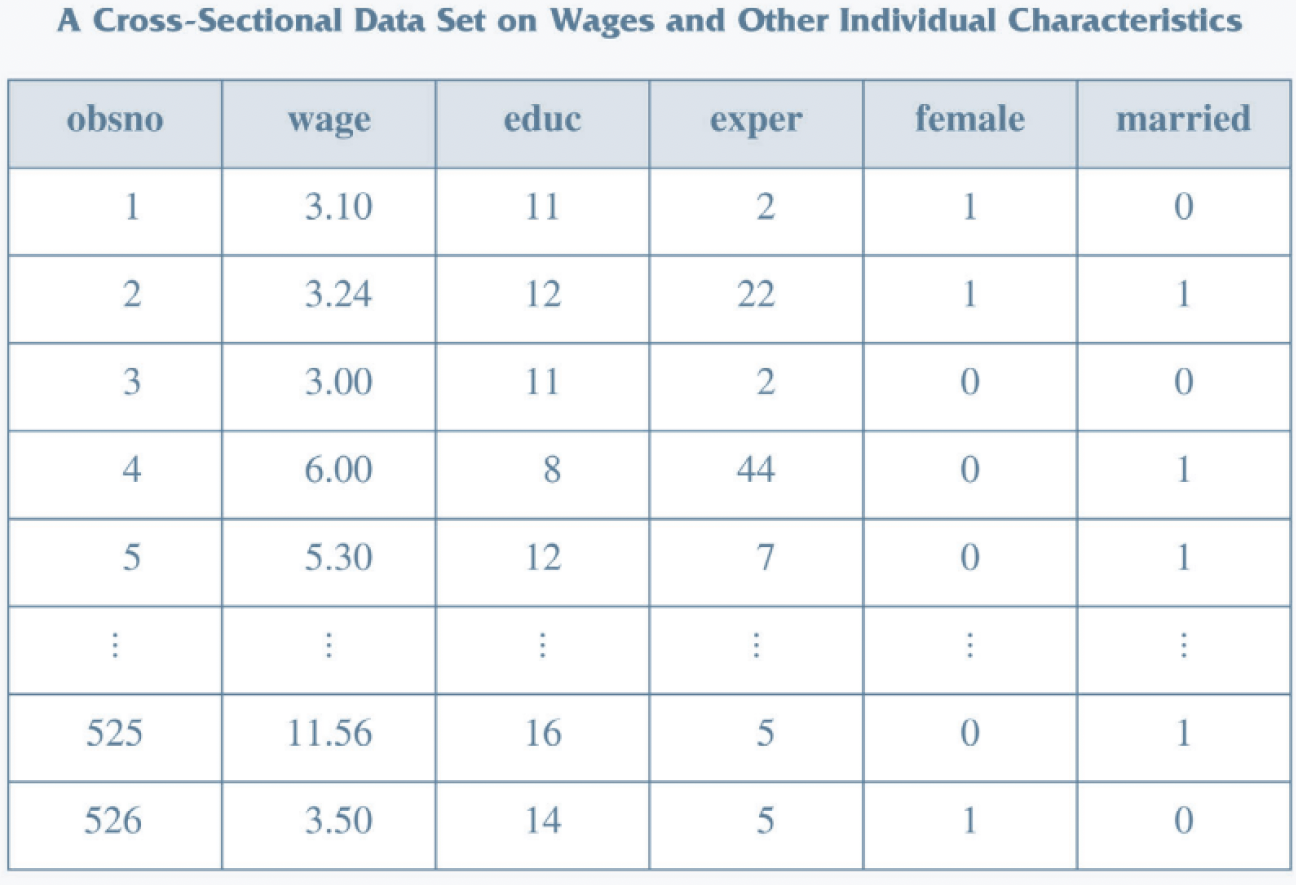
\includegraphics[scale=.4]{images/crossex0.png}
\end{figure}
\end{column}
\end{columns}
\end{frame}


\begin{frame}{Pooled Cross-Section}
 \begin{columns}
\begin{column}{0.3\textwidth}
A natural extension of the cross-sectional data is the \textbf{pooled cross-sectional data} --- where cross-sectional data is gathered at multiple points in time and where each cross-sectional study is independent of the others.\\[1em]

In other words, different samples of subjects or entities are observed during each data collection period.

\end{column}
\begin{column}{0.7\textwidth}
\begin{figure}
  \centering
         \vspace{-1mm}
        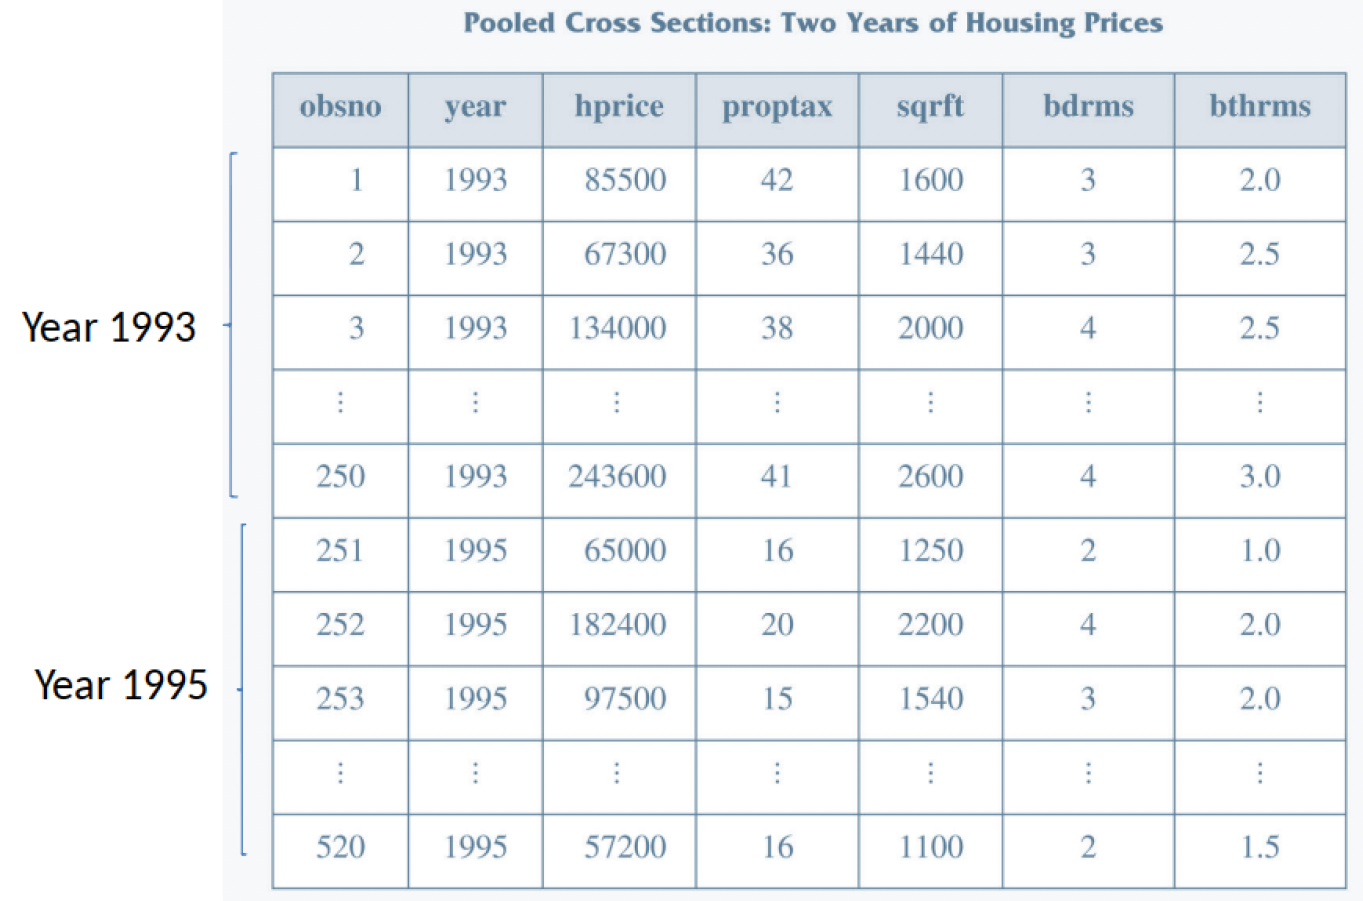
\includegraphics[scale=.4]{images/repcrossex0.png}
\end{figure}
\end{column}
\end{columns}
\end{frame}


\begin{frame}{Pooled Cross-Section}
Many surveys, randomly sampling individuals, families, or firms are repeated at regular time intervals (e.g., CPS in the U.S.)\\[1em]

Pooled together $\Longrightarrow$ independently pooled cross section

\begin{columns} 
% Column 1
    \begin{column}{.5\textwidth}
        \begin{center}
            \textbf{Pros}
        \end{center}
        \begin{itemize}
            \item Statistical inference is the same as for cross-sectional methods
            \item Larger sample size (i.e., lower standard errors)
            \item Enables us to estimate trends conditional on explanatory variables.
            \item Enables us to estimate how the effect of one factor has changed over time (e.g., how did the gender wage gap change?)
        \end{itemize}
    \end{column}
    \begin{column}{.5\textwidth}
        \begin{center}
            \textbf{Cons}
        \end{center}
        \begin{itemize}
        \setcounter{enumi}{7}
            \item Populations have different distribution across time periods, thus they are not \textit{identically} distributed\\
            $\rightarrow$ we can allow the intercept to differ across periods! \textit{(how?)}
        \end{itemize}

    \end{column}
\end{columns}
\end{frame}

\begin{frame}{Fertility over time}
\begin{figure}
  \centering
         \vspace{-1mm}
         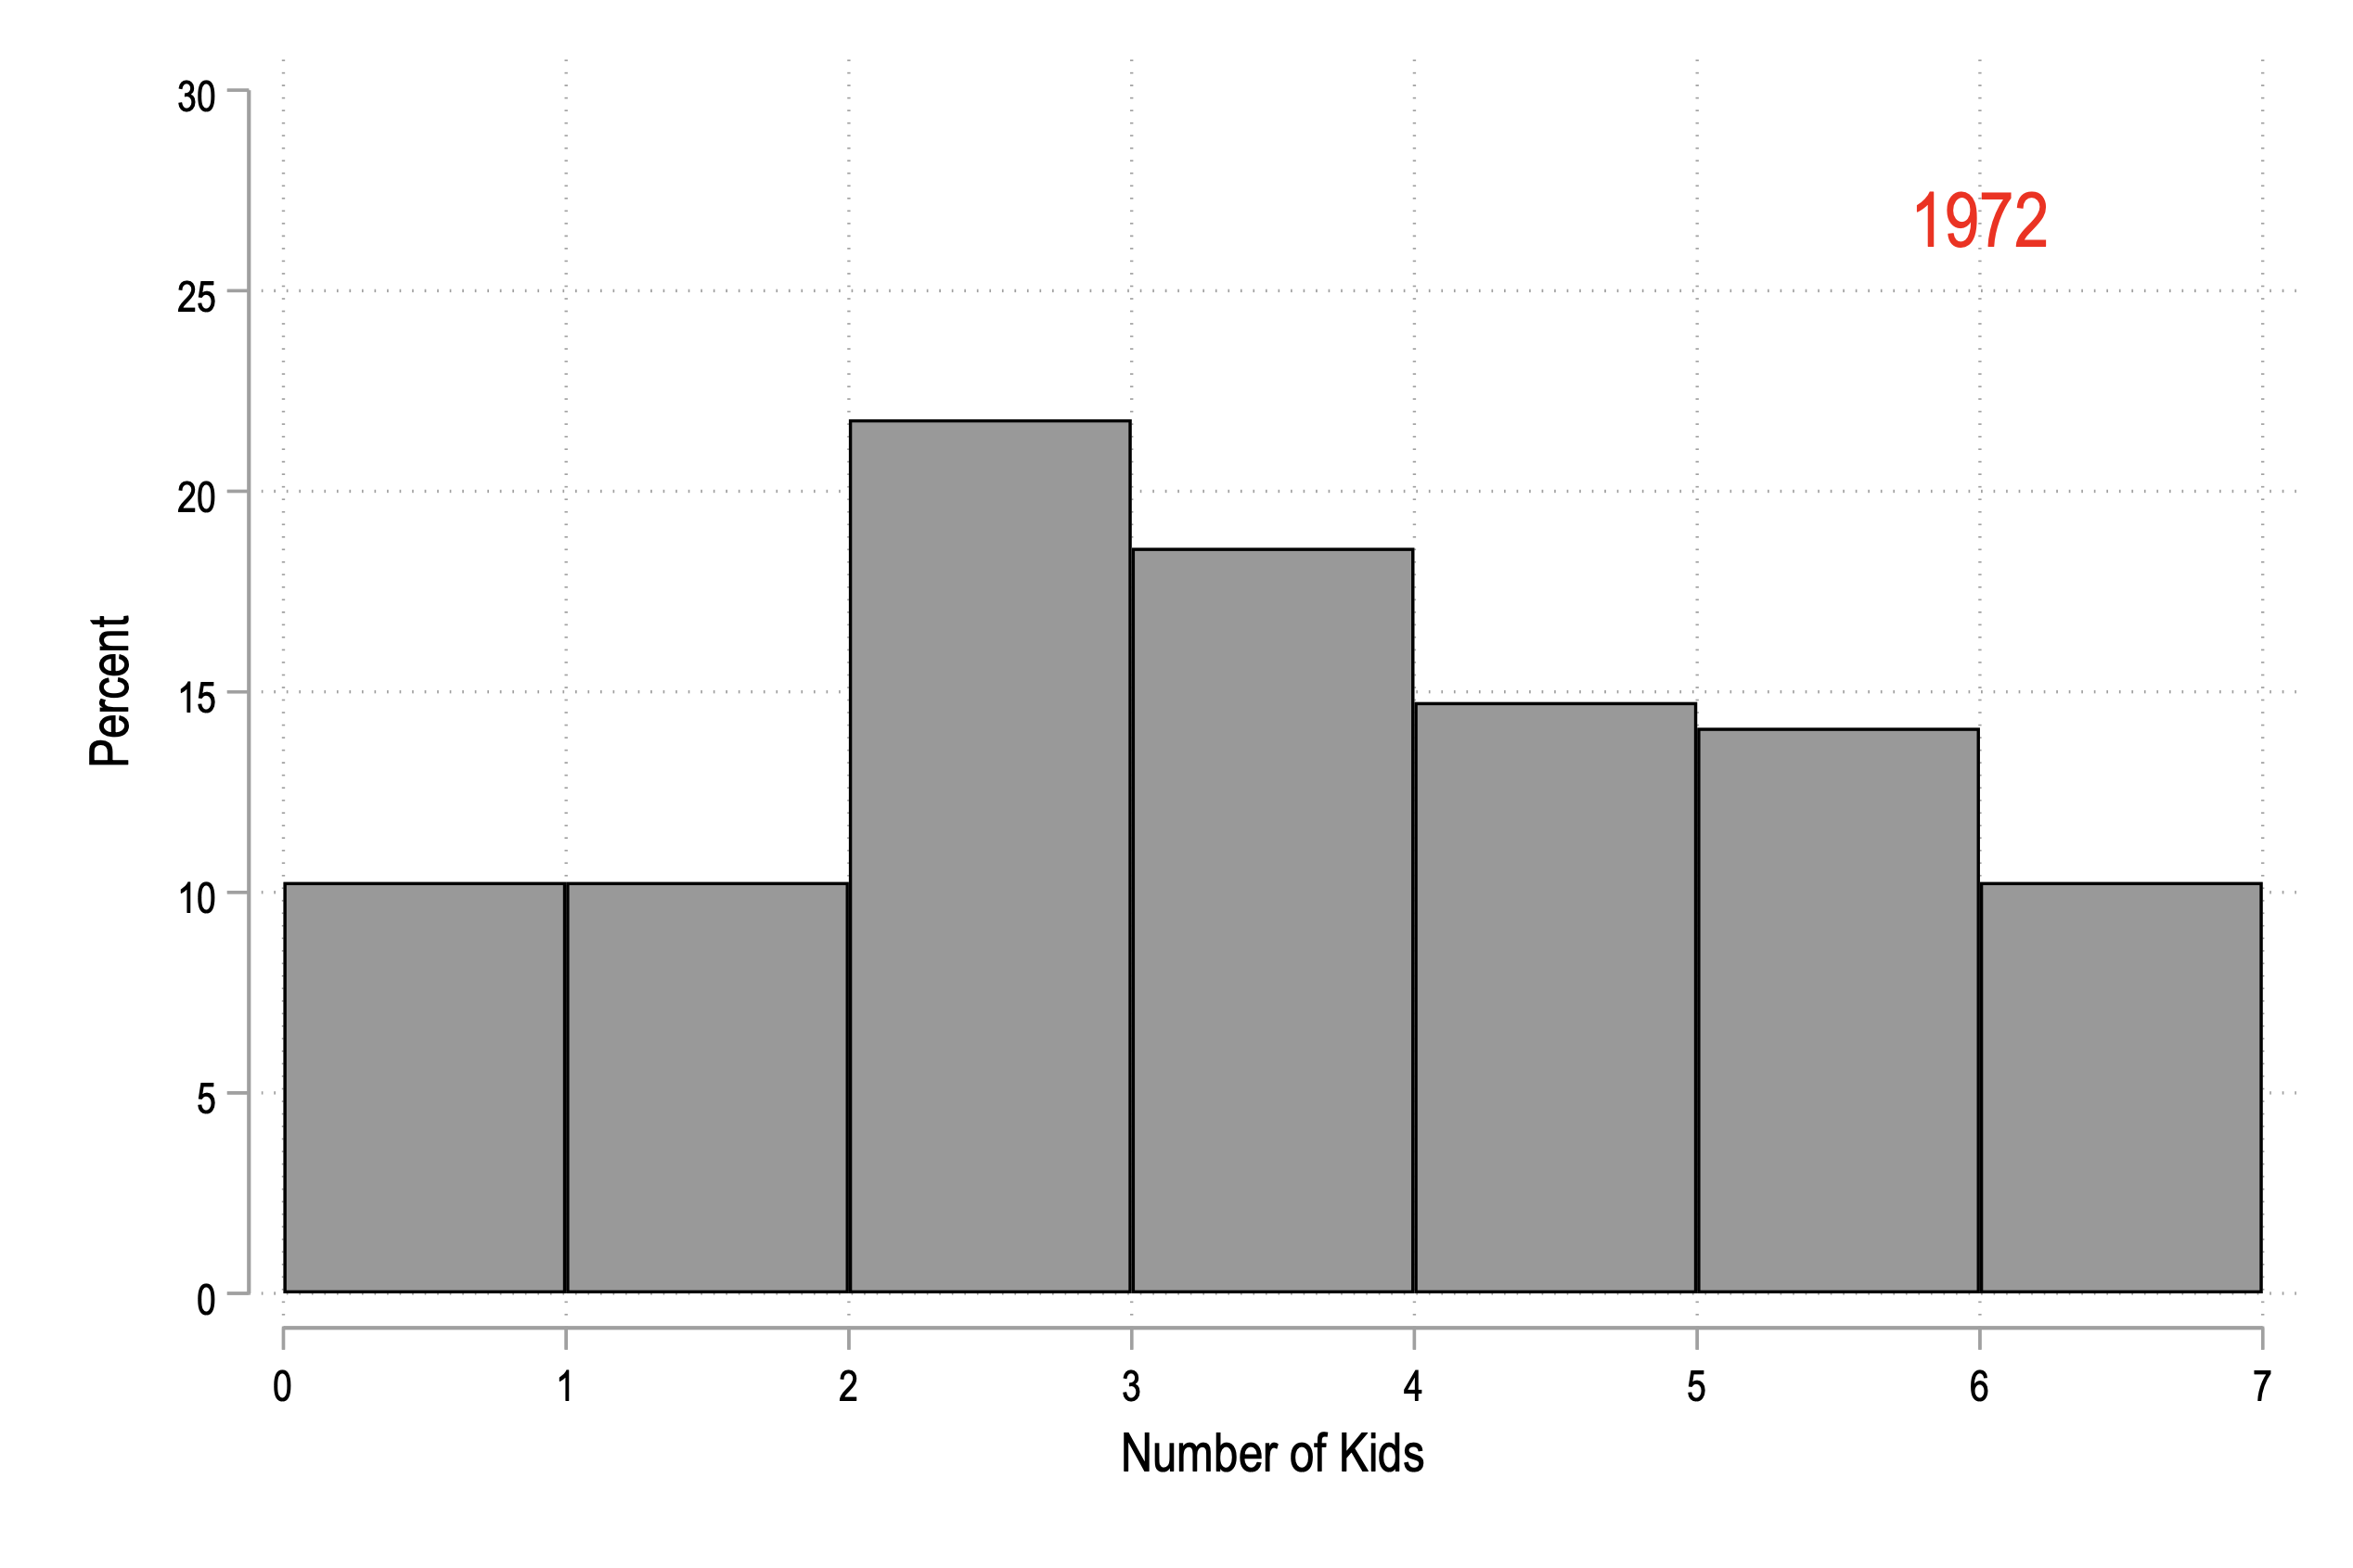
\includegraphics[width=.8\linewidth]{images/cps72.png}
\end{figure}
\end{frame}

\begin{frame}{Fertility over time}
\begin{figure}
  \centering
         \vspace{-1mm}
         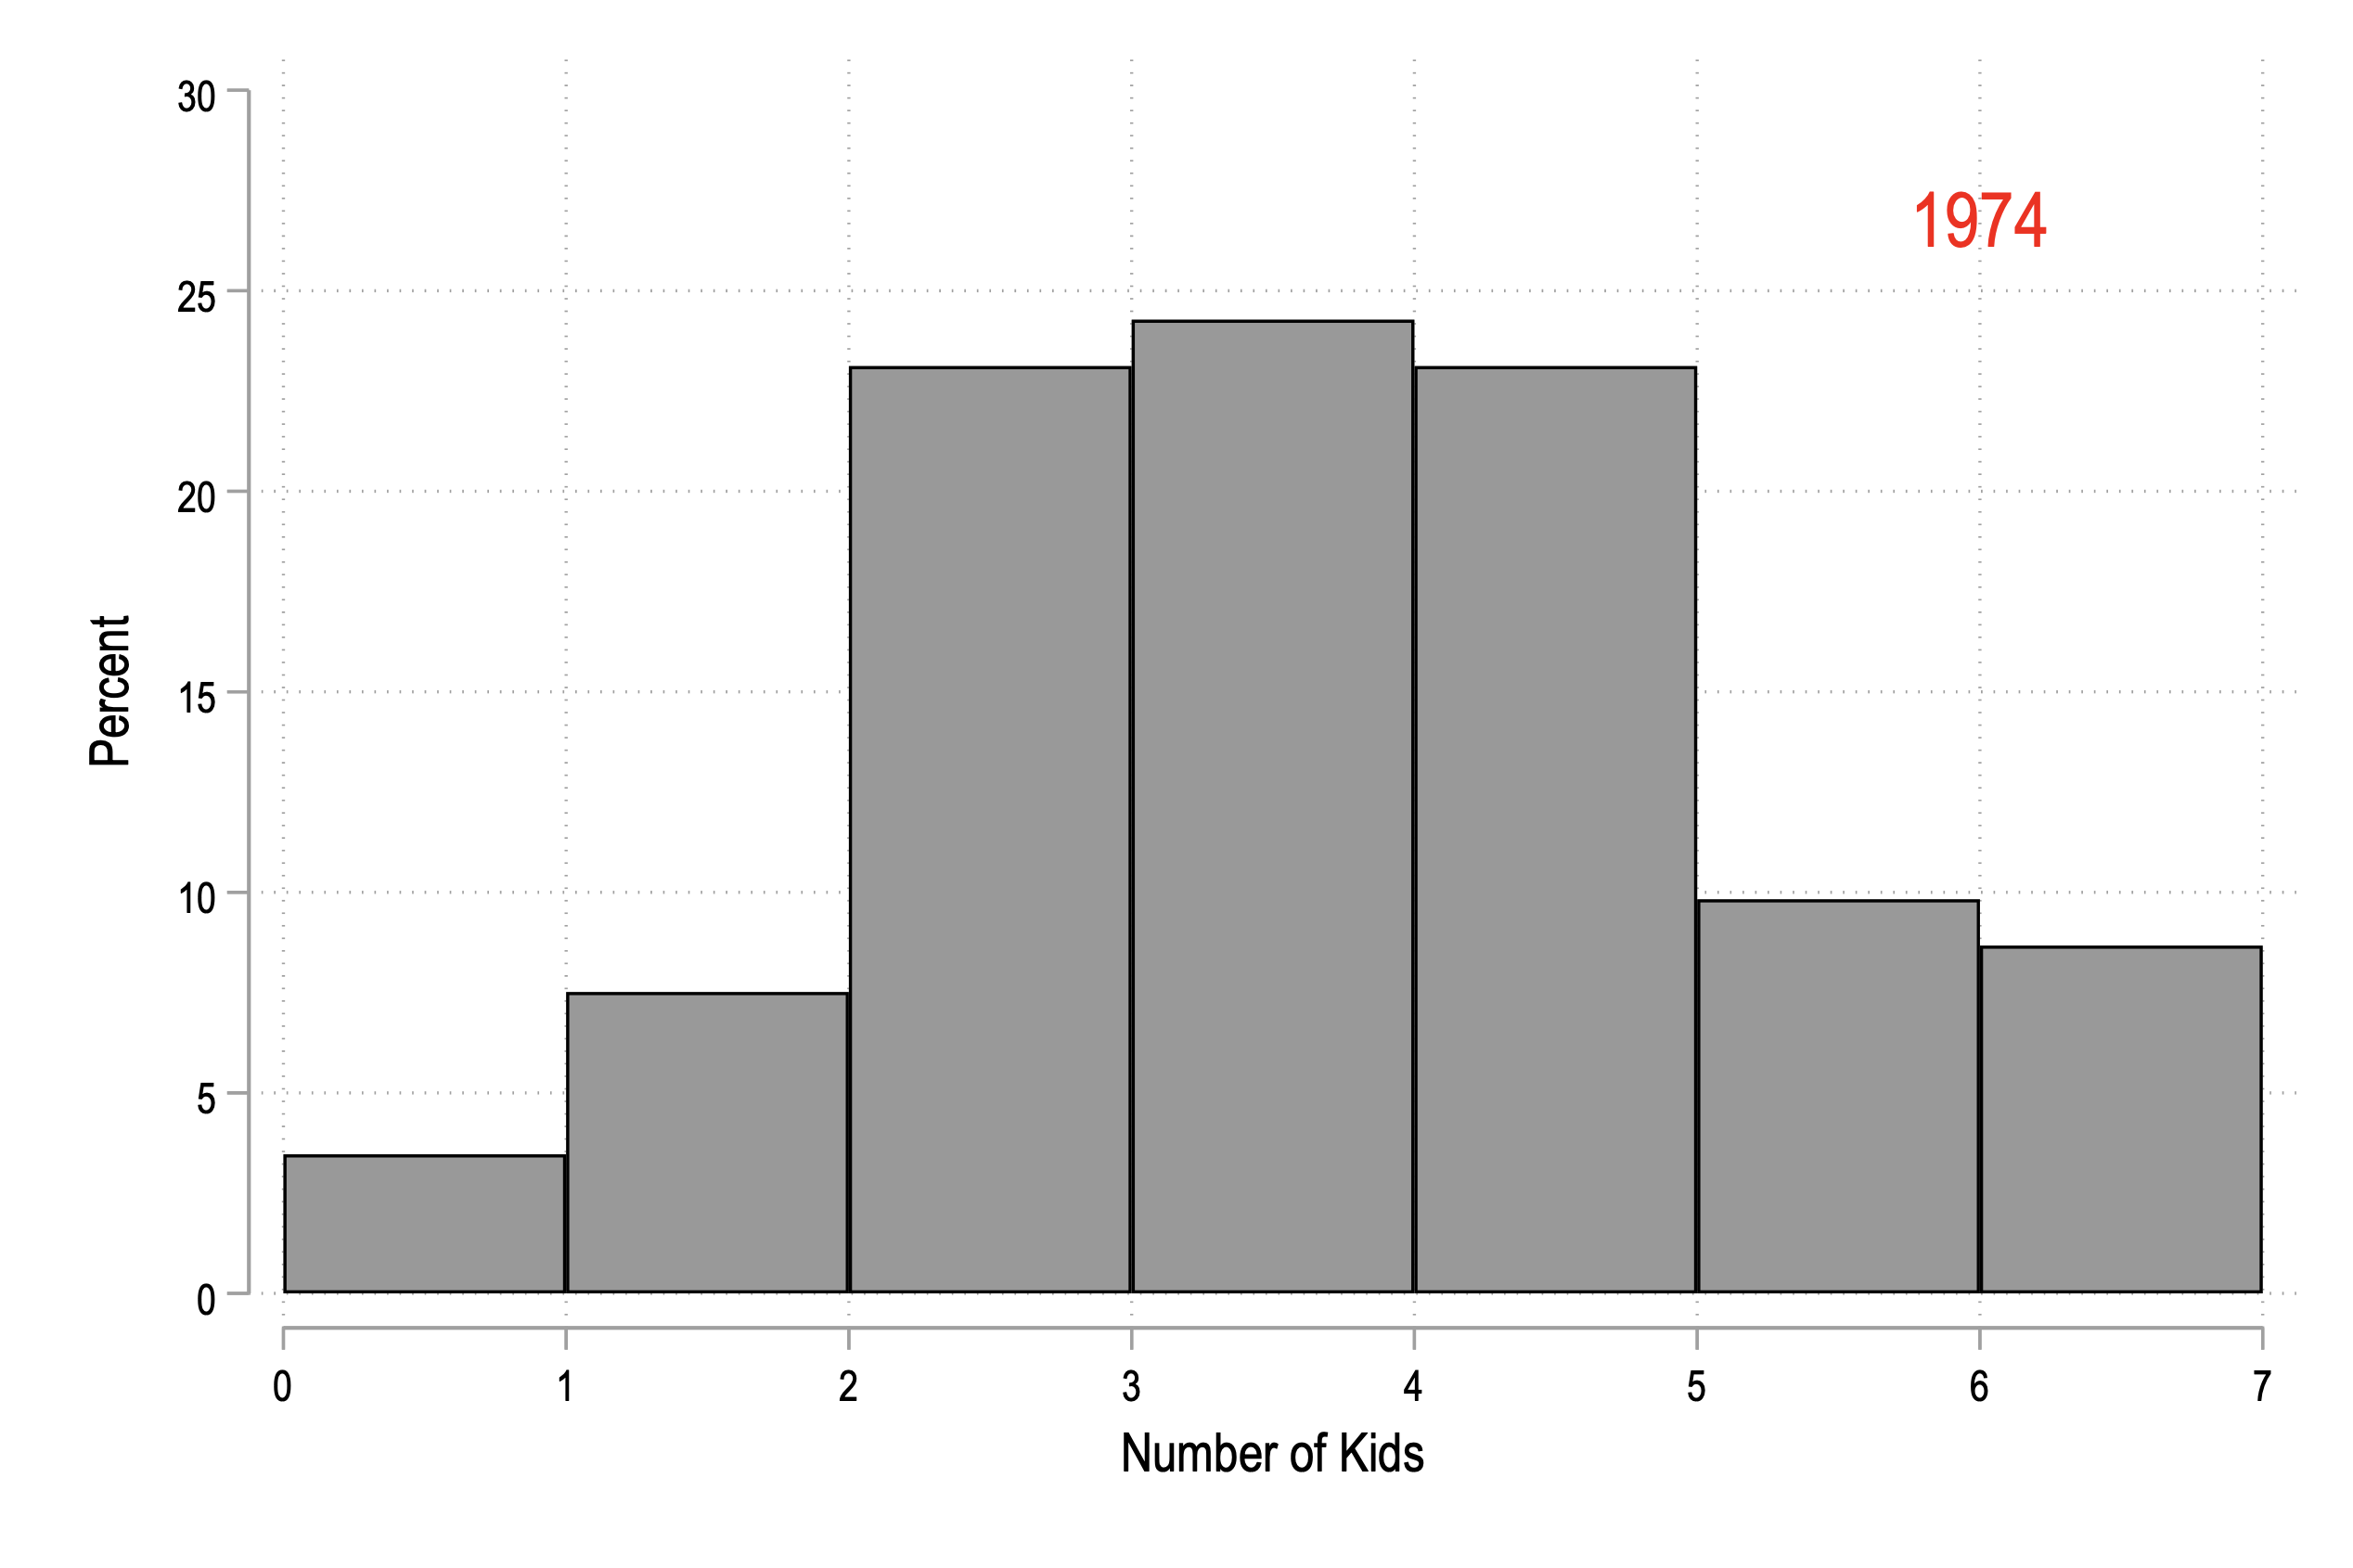
\includegraphics[width=.8\linewidth]{images/cps74.png}
\end{figure}
\end{frame}

\begin{frame}{Fertility over time}
\begin{figure}
  \centering
         \vspace{-1mm}
         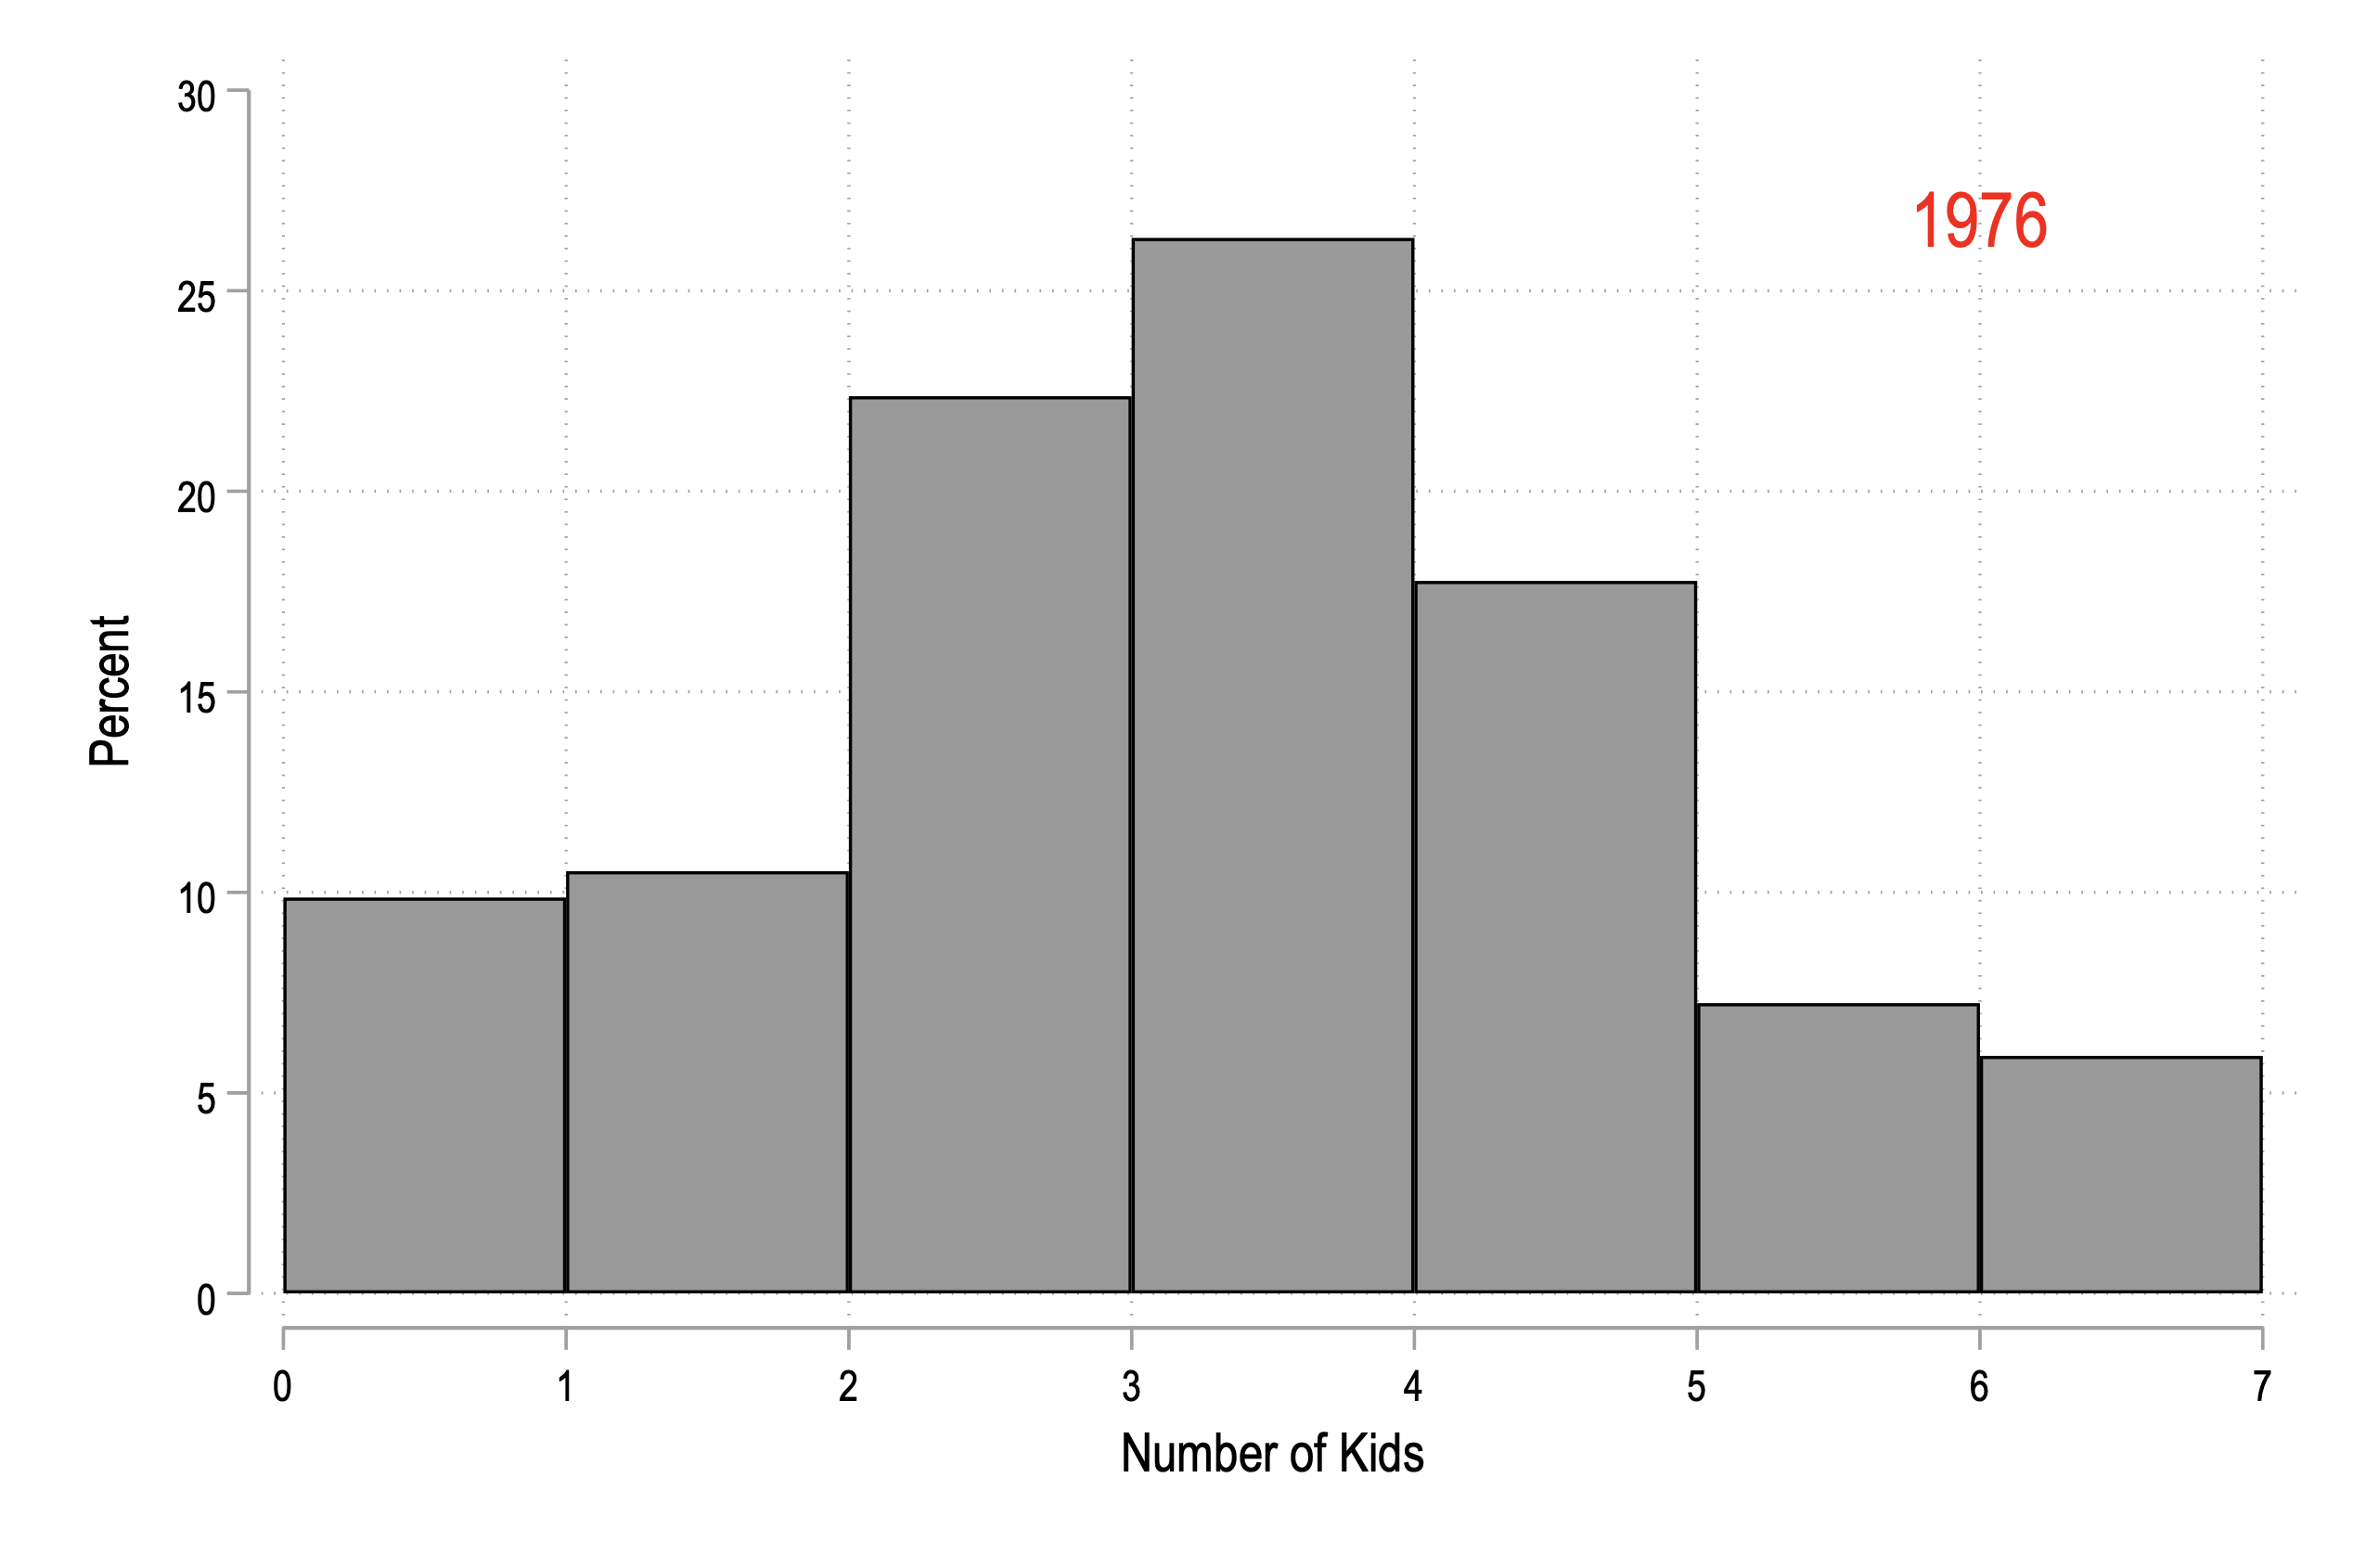
\includegraphics[width=.8\linewidth]{images/cps76.png}
\end{figure}
\end{frame}


\begin{frame}{Fertility over time}
\begin{figure}
  \centering
         \vspace{-1mm}
         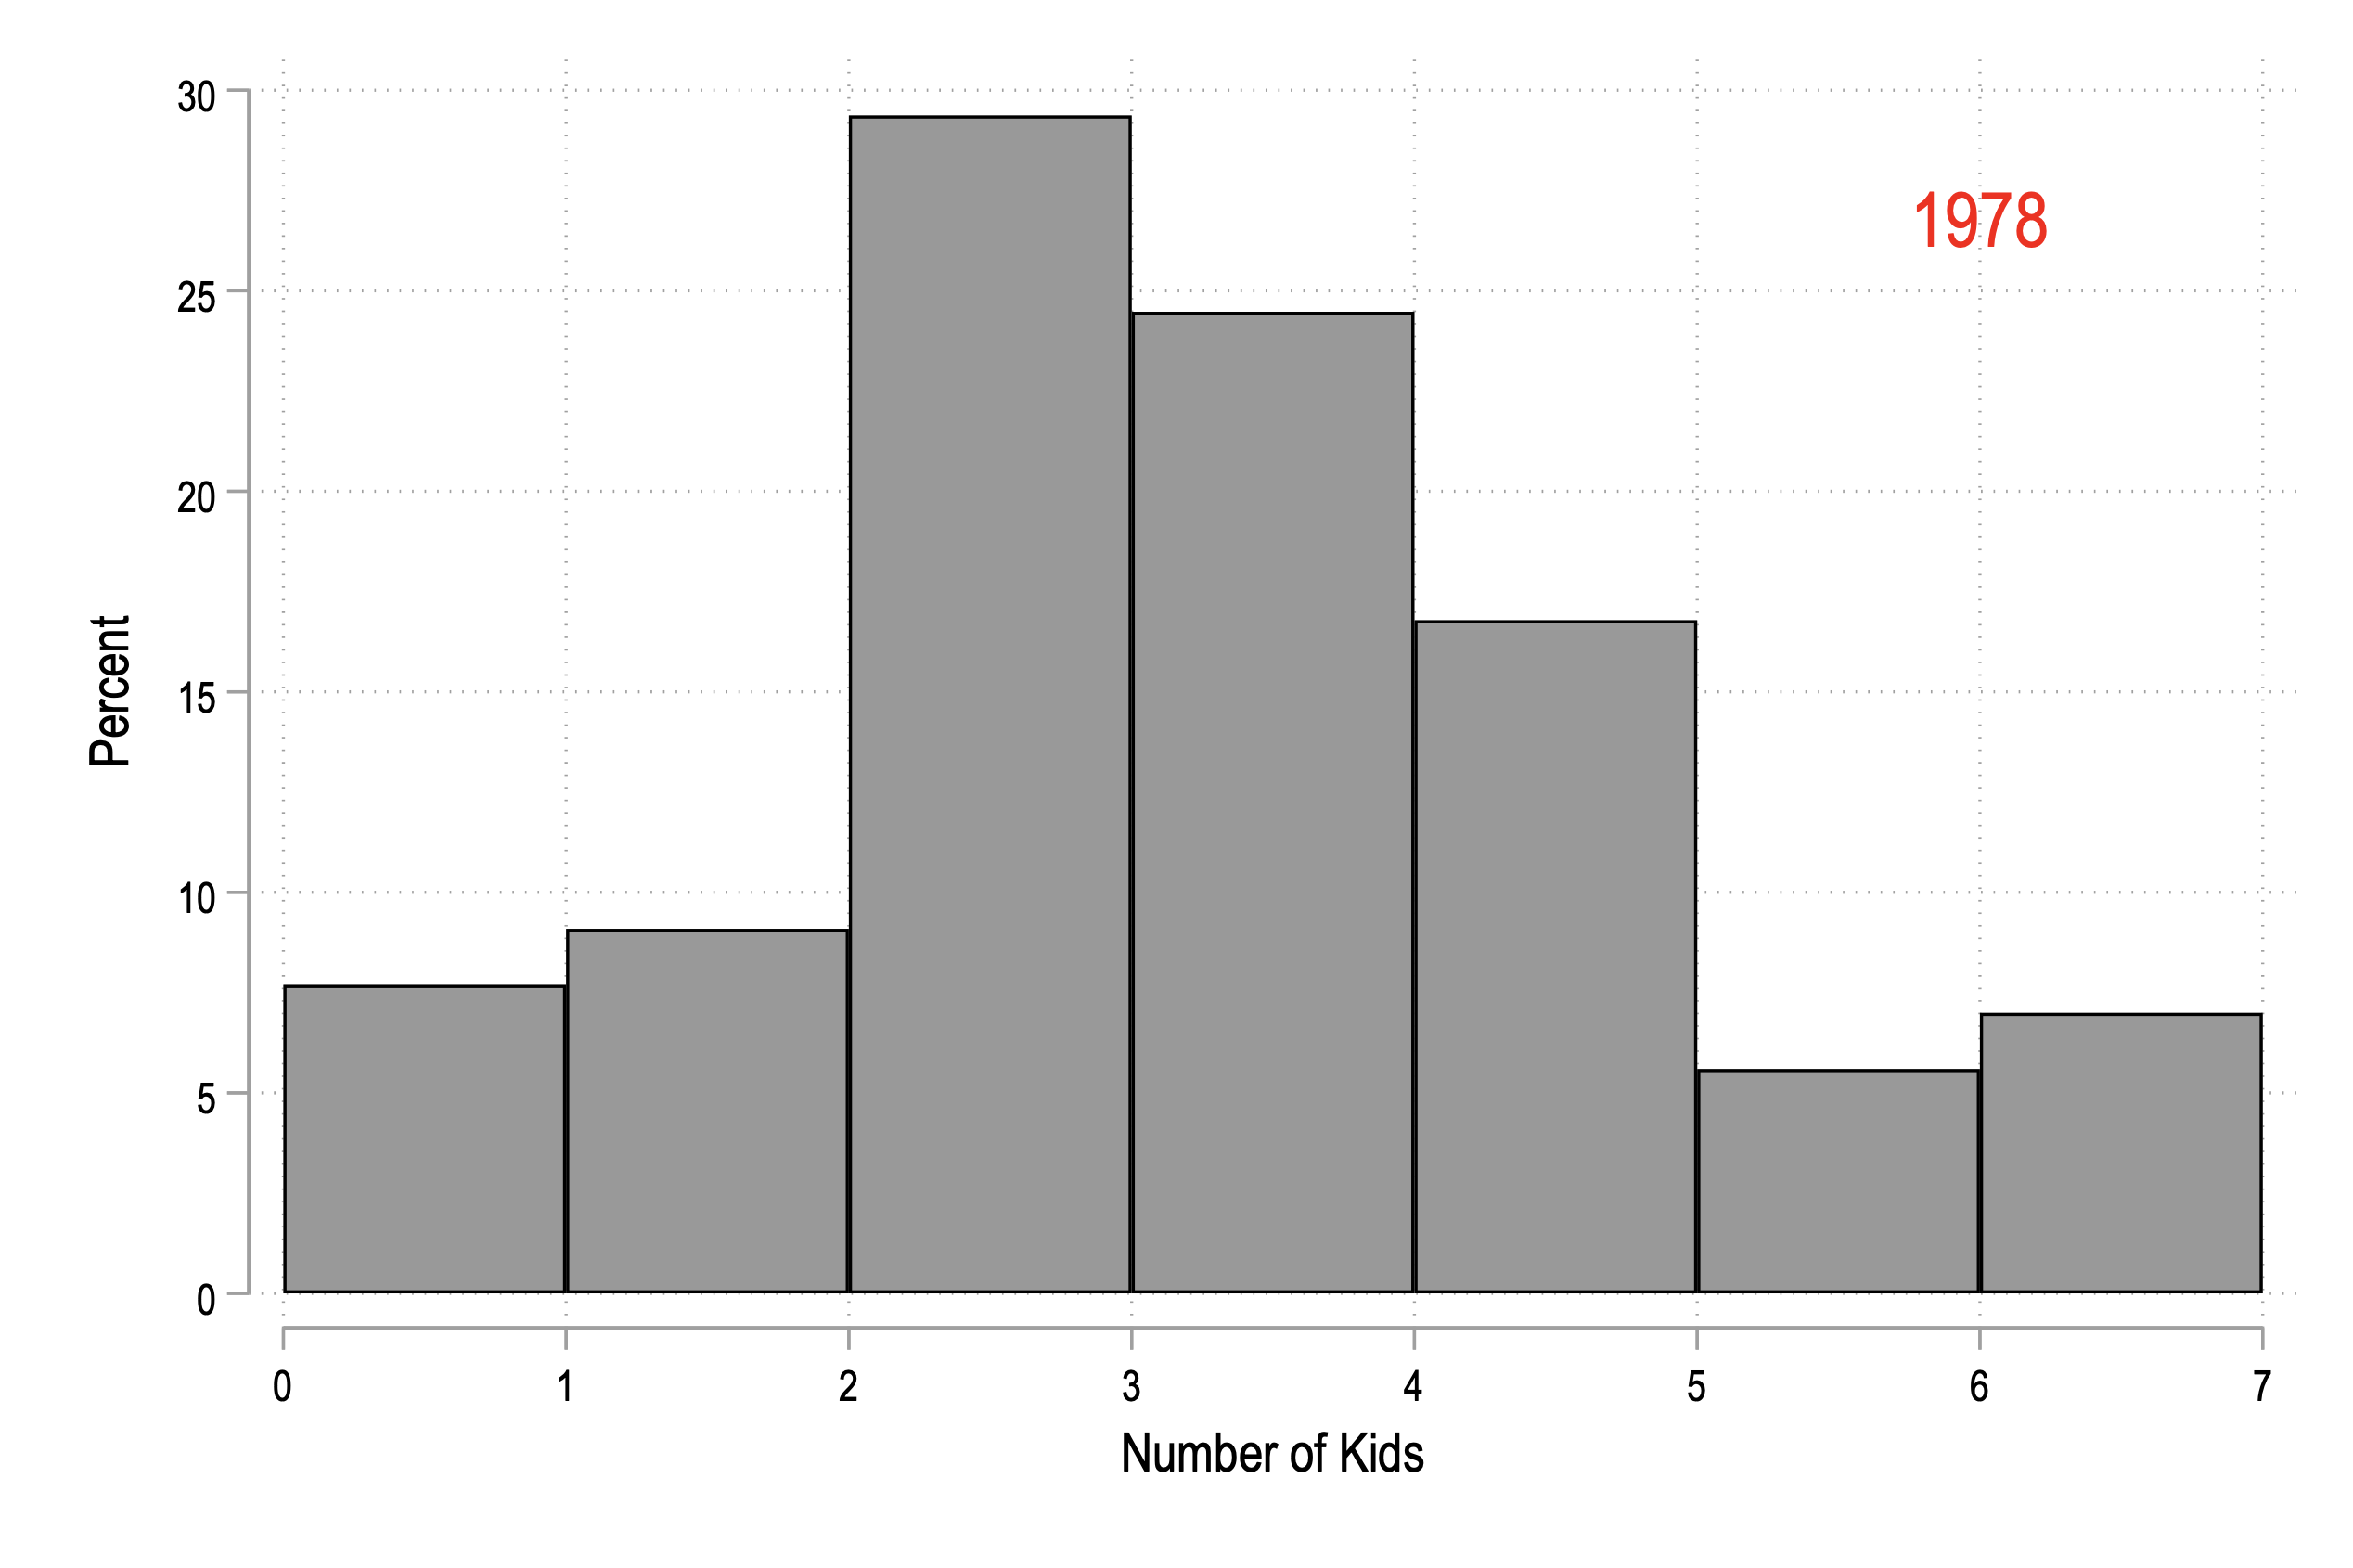
\includegraphics[width=.8\linewidth]{images/cps78.png}
\end{figure}
\end{frame}


\begin{frame}{Fertility over time}
\begin{figure}
  \centering
         \vspace{-1mm}
         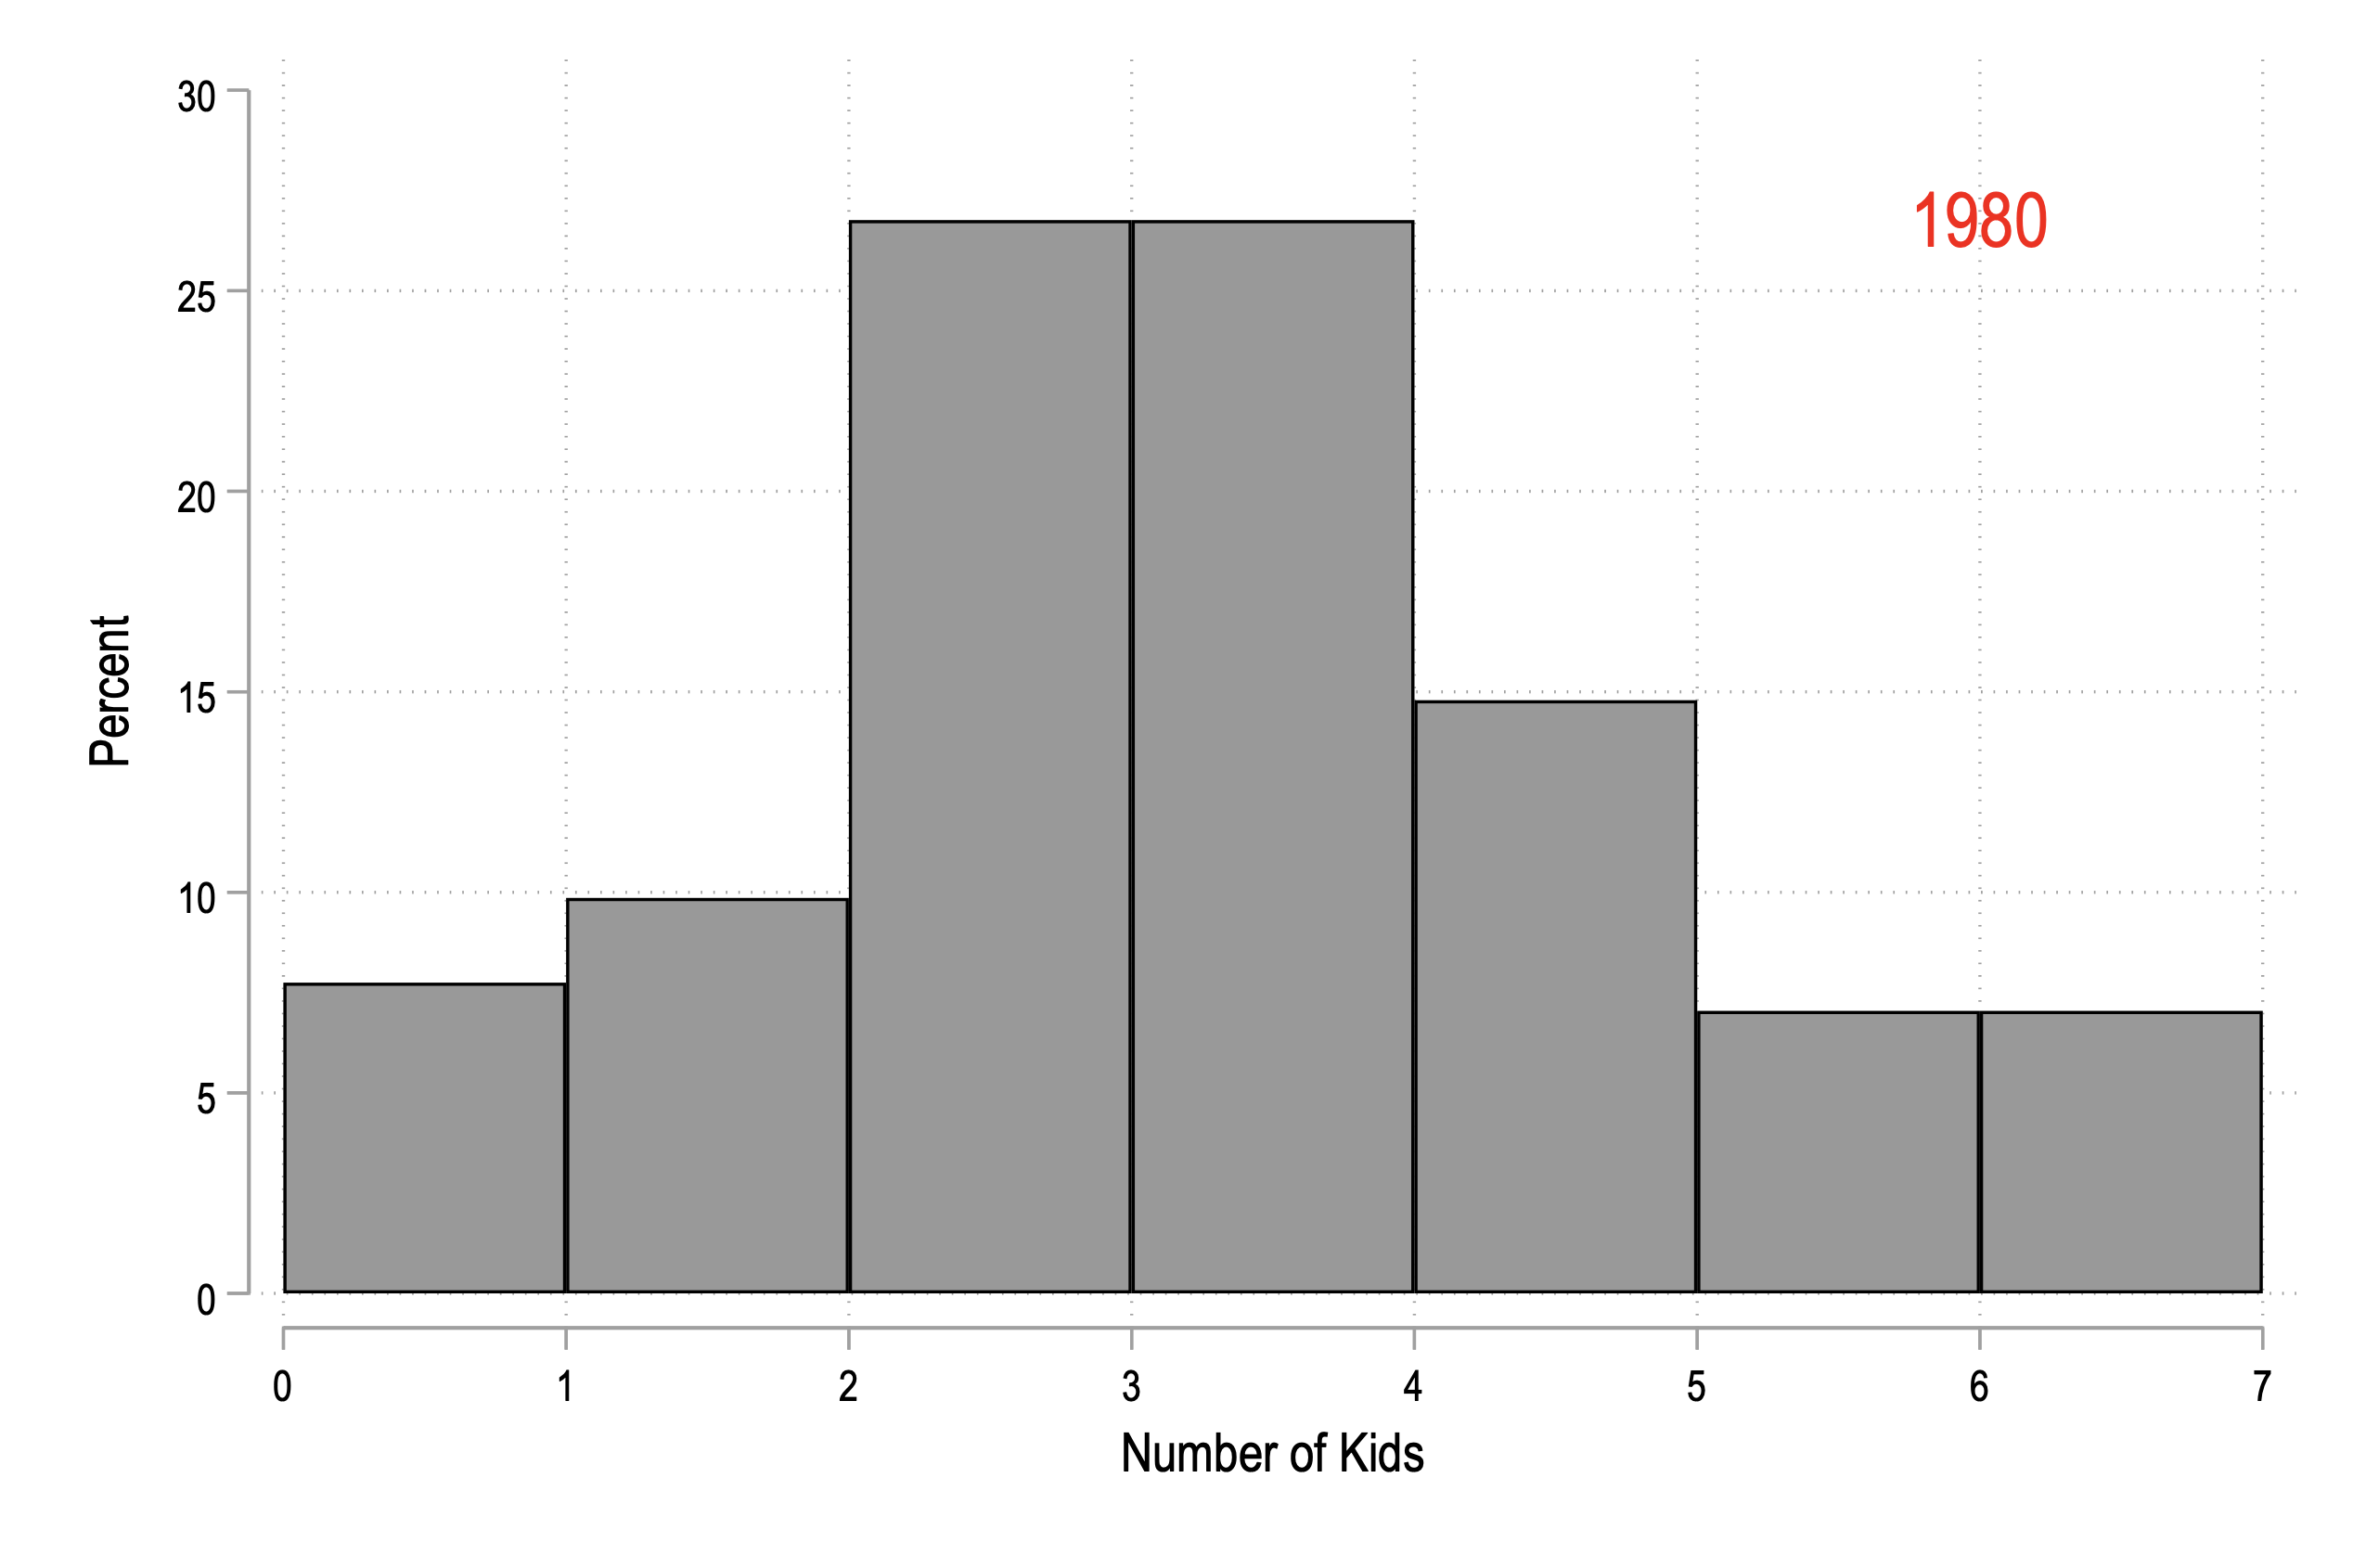
\includegraphics[width=.8\linewidth]{images/cps80.png}
\end{figure}
\end{frame}

\begin{frame}{Fertility over time}
\begin{figure}
  \centering
         \vspace{-1mm}
         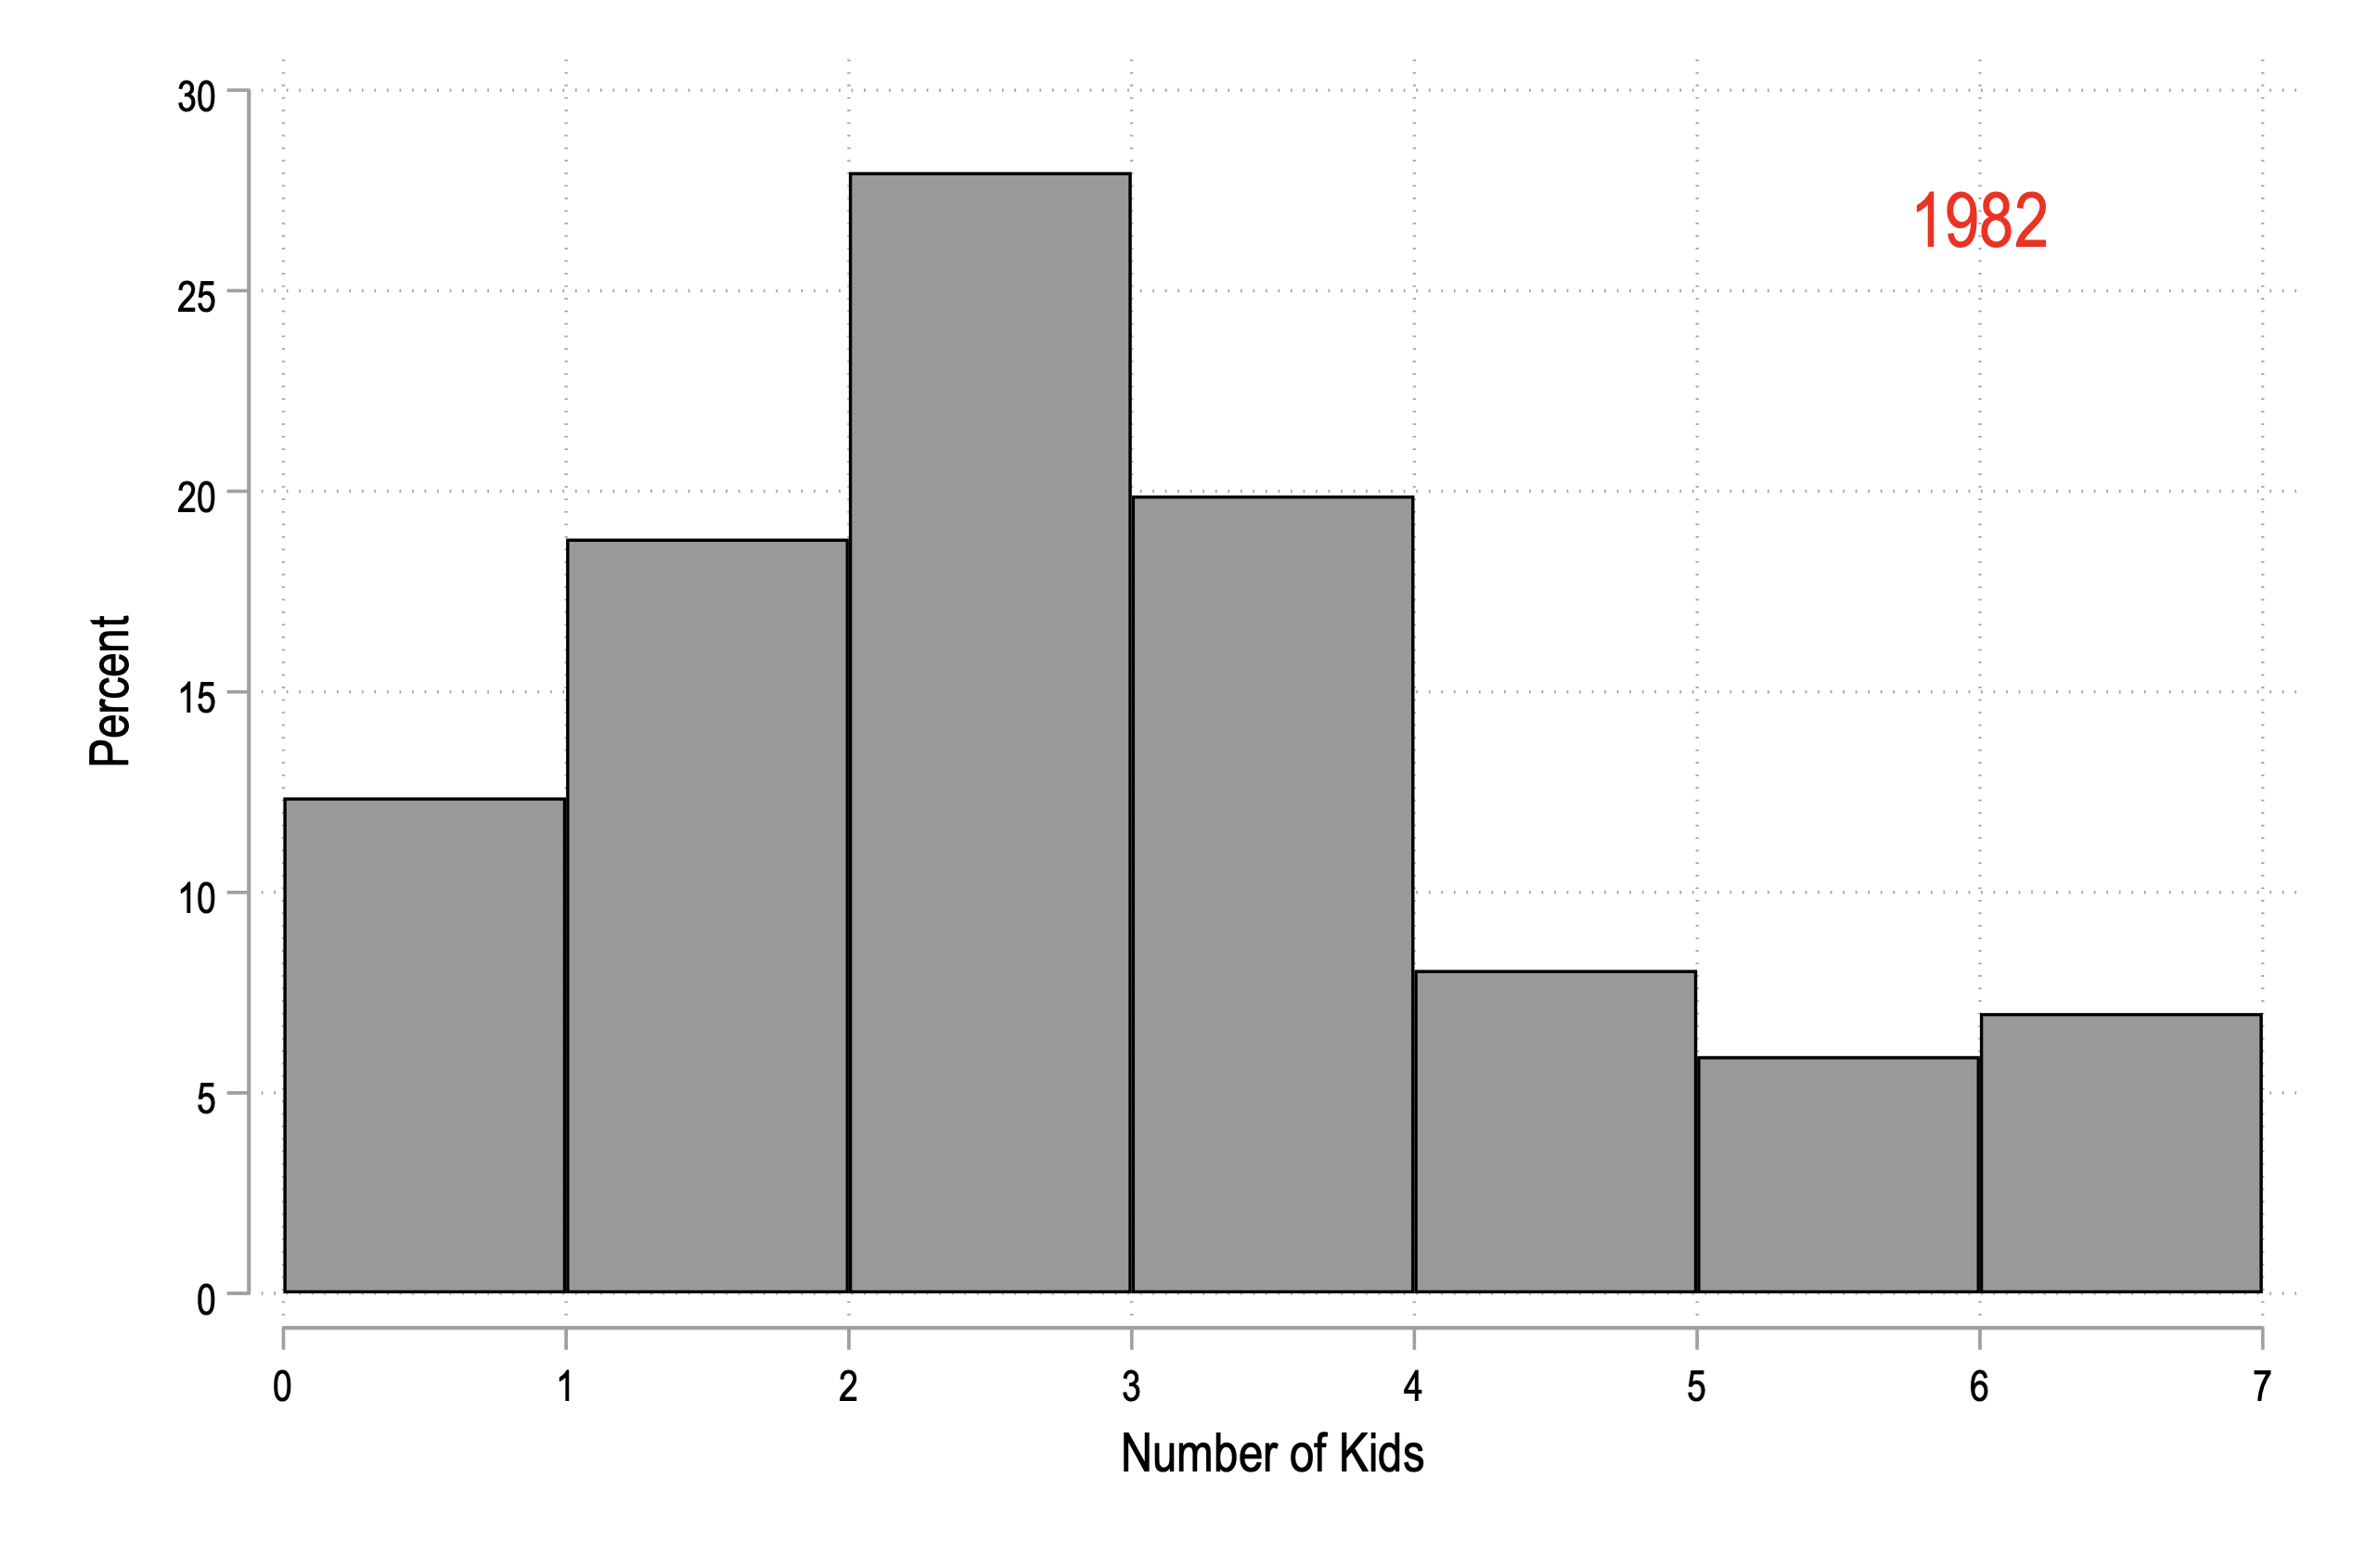
\includegraphics[width=.8\linewidth]{images/cps82.png}
\end{figure}
\end{frame}

\begin{frame}{Fertility over time}
\begin{figure}
  \centering
         \vspace{-1mm}
         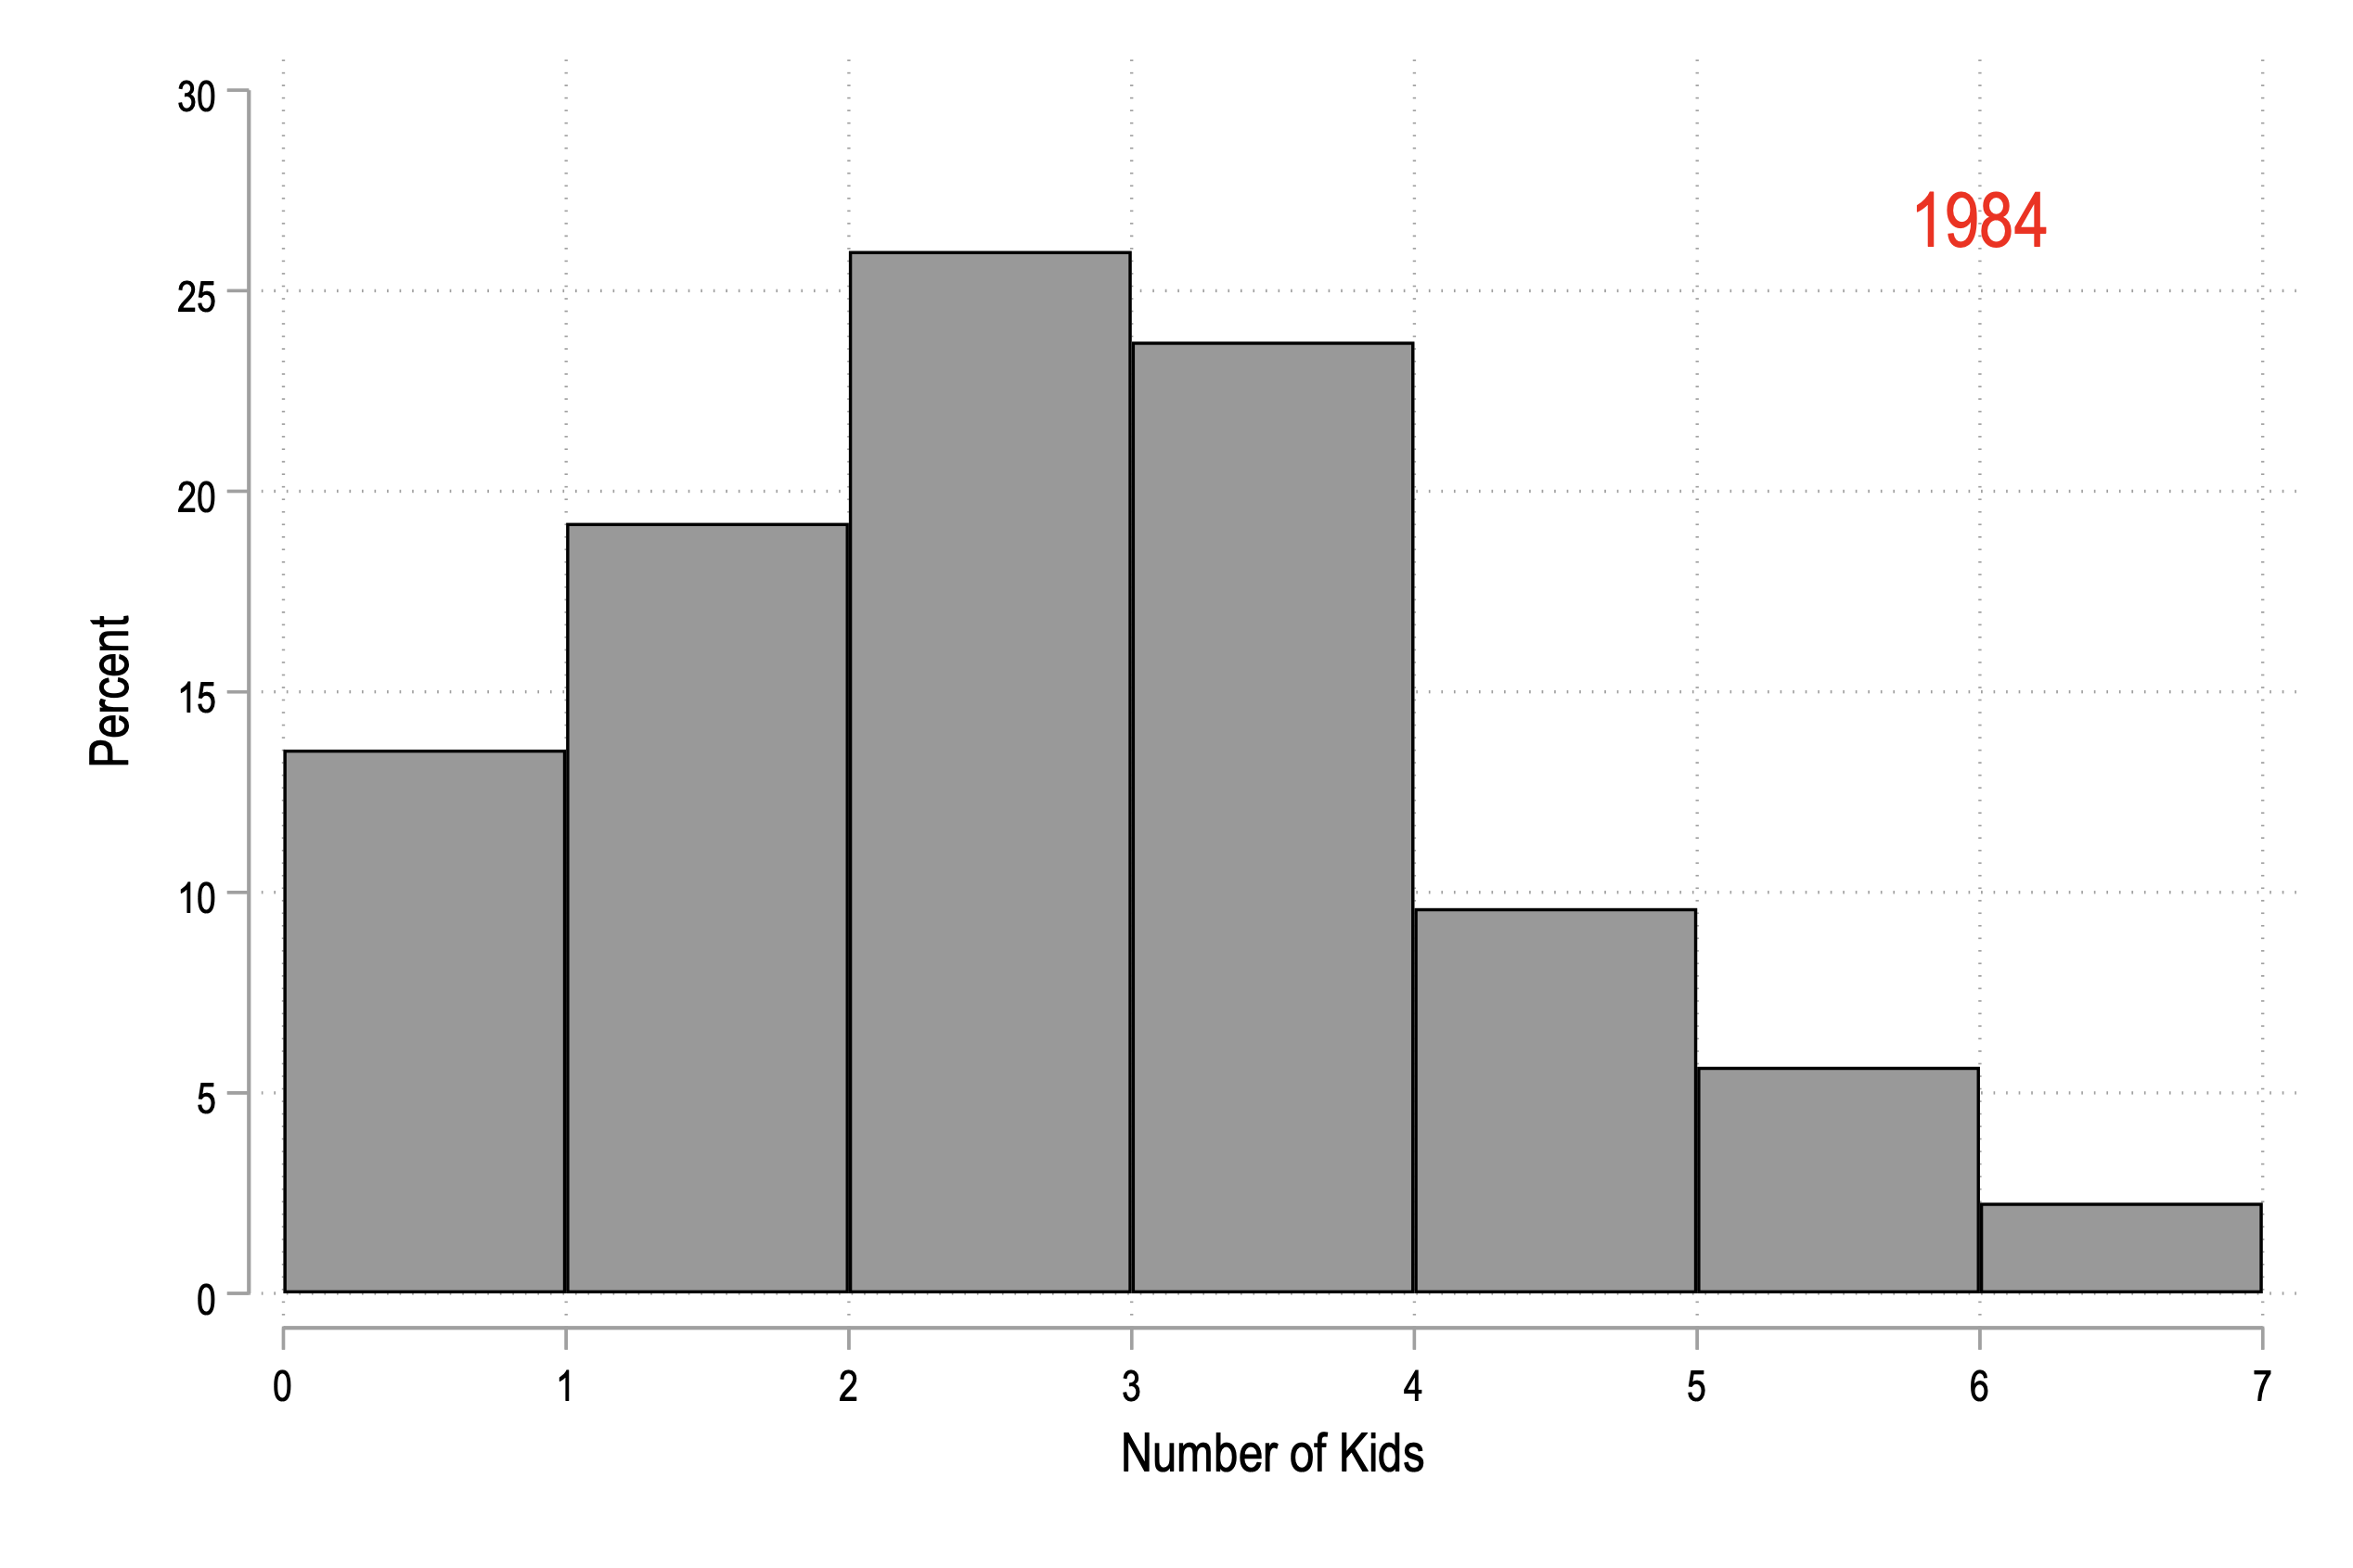
\includegraphics[width=.8\linewidth]{images/cps84.png}
\end{figure}
\end{frame}




\begin{frame}{Fertility over time}
 \begin{columns}
\begin{column}{0.3\textwidth}
From Lecture 7 --- We can use year-specific intercepts by including year-specific dummies\\[1em]
Remember from Lecture 7 ---  the base year here is...?\\[1em]

Sharp decline in the number of kids per woman in the 1980s which is $not$ explained by changes in main demographics

\end{column}
\begin{column}{0.7\textwidth}
\begin{figure}
  \centering
         \vspace{-1mm}
         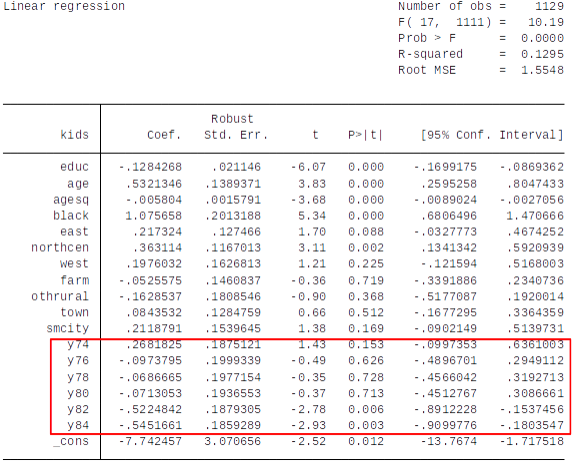
\includegraphics[width=.9\linewidth]{images/cps1.png}
\end{figure}
\end{column}
\end{columns}
\end{frame}


\begin{frame}{Gender Gap}
As in Lecture 7, we can allow for different intercepts \textit{and} slopes gradients by interacting a dummy and a continuous variable\\[1em]

\textbf{Example:}
\begin{itemize}
    \item Pooled 2 cross-sectional datasets (1978 and 1985)
    \item Data on wages, educational attainment, and gender
    \item \underline{\textit{Questions:}}
    \begin{itemize}
        \item Did the gender wage gap change from 1978 to 1985?
        \item Did the return to education change from 1978 to 1985?
\end{itemize}
\end{itemize}
\begin{eqnarray*}
    &ln(wage) &= \beta_0 + \beta_1 \mathds{1}_{1985} + \beta_2 Educ + \beta_3 (Educ \times \mathds{1}_{1985} ) + \beta_4 Female + \beta_5 (Female \times \mathds{1}_{1985} ) \\
    &{} &+ \beta_6 Experience  + \beta_7 {Experience}^2 + \beta_8 Union + u
\end{eqnarray*}
\end{frame}

\begin{frame}{Gender Gap}
\begin{figure}
  \centering
         \vspace{-1mm}
         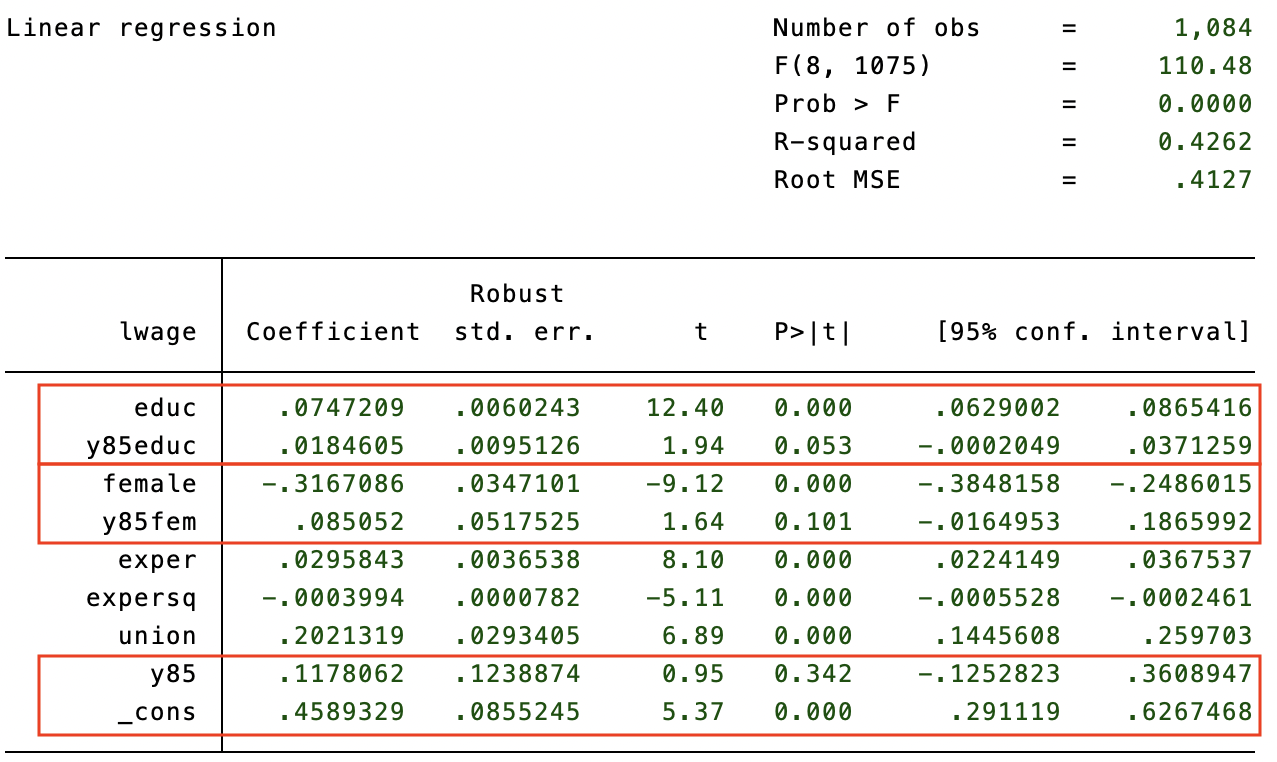
\includegraphics[width=.8\linewidth]{images/gendergap0.png}
\end{figure}
\end{frame}


\begin{frame}{Testing Differences in Pooled regressions}
When \textit{all} variables are interacted with the time dummies, the regression specification is equivalent to estimating separate regressions --- one for each year.\\[1em]

As in Lecture 7, one can test whether the population regression lines differ across two different years by running a simple \textbf{Chow test}.\\[1em]

First, run the fully interacted model ($year_1$ serves as the base period)
\begin{equation*}
    Y_i = \beta_0 + \beta_1 X_{1i} + \cdots + \beta_k X_{ki} + \beta_{k+1} \mathds{1}_{year_2} + \beta_{k+2}  (\mathds{1}_{year_2} \times X_{1i}) + \cdots + \beta_{2k+1}(\mathds{1}_{year_2}\times X_{ki})  + u_i
\end{equation*}

Then test $\beta_{k+1}=\beta_{k+2}=\cdots=\beta_{2k+1}=0$\\[1em]

We can also test whether the intercepts differ between the 2 groups ($H_0: \beta_{k+1}=0$) or whether the slopes differ ($H_0: \beta_{k+2}=\cdots=\beta_{2k+1}=0$)
\end{frame}


\section{From Pooled to Panel Data}

\begin{frame}
  \vfill
  \centering
    {\huge \color{blue} \textit{From Pooled to Panel Data}}
  \vfill
\end{frame}

\begin{frame}{What is a panel dataset?}
A panel dataset (also called longitudinal data) contains observations on multiple entities (e.g., individuals, states, companies, etc.), observed at two or more points in time (e.g., days, months, years, decades, etc.).\\[1em]

For example,
\begin{itemize}
    \item Data on 420 California school districts in 1999 and again in 2000, for 840 observations total.
    \item Data on 50 U.S. states, each state is observed in 3 years, for a total of 150 observations.
    \item Data on 1000 individuals in four different months, for 4000 observations total.
\end{itemize}\\[1em]

Panel data with $k$ regressors: $\{X_{1,it}, X_{2,it}, ..., X_{k,it}, Y_{it}\}$ where $i=1, \dots, n$ and $t=1, \dots, T$\\[1em]

When all $k+1$ variables are observed for all units $i$ at all points in time $t$ (i.e., no missing observations), we say the panel is balanced.
\end{frame}




\begin{frame}{Panel Data}
 \begin{columns}
\begin{column}{0.3\textwidth}
\textbf{Panel} data is also known as \textbf{longitudinal} data or \textbf{cross-sectional time-series} data\\[1em]

It involves observations of multiple entities over multiple time periods.\\[1em]

We say a panel is \textbf{balanced} if all entities are observed in each time period, and there are no missing observations.\\[1em]

We will focus on the case where $N>>T$
\end{column}
\begin{column}{0.7\textwidth}
\begin{figure}
  \centering
         \vspace{-1mm}
         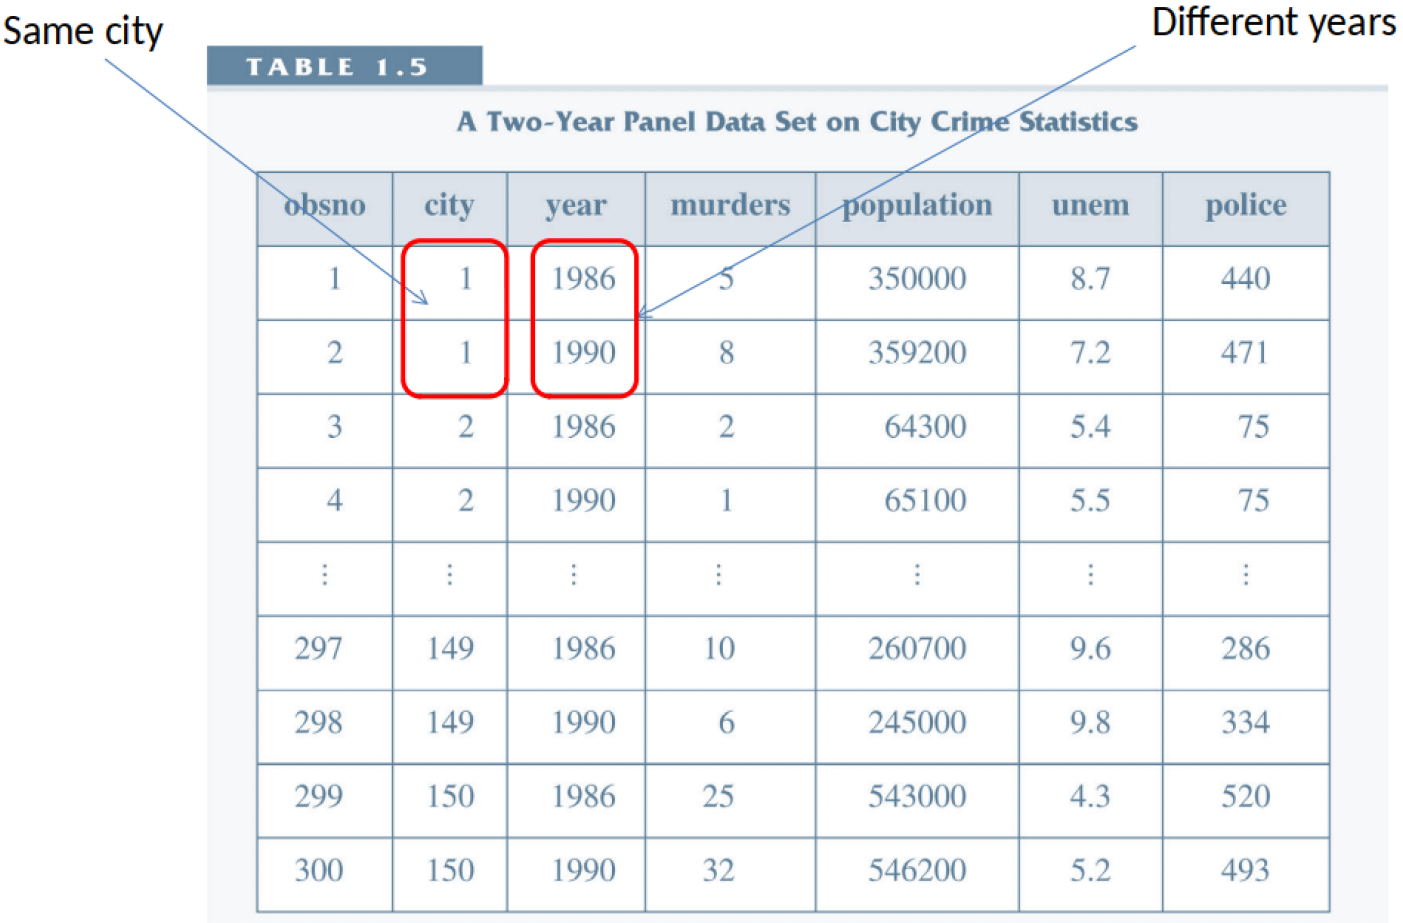
\includegraphics[width=.9\linewidth]{images/panelex0.png}
\end{figure}
\end{column}
\end{columns}
\end{frame}


% Types of datasets
% Pooled data models
% Chow test
% Hicks 1994

\begin{frame}{Why are panel data useful? }
With panel data, we can control for factors that:
\begin{itemize}
    \item Vary across units but not over time (in the sample period) {\footnotesize $\longleftarrow$ (we will focus on that case first)}
    \item Vary over time (in the sample period) but not across units
\end{itemize}\\[1em]
These `black boxes' could contain omitted variables, which are typically unobserved or unmeasured --- and therefore cannot be included in the regression using multiple regression.\\[1em]

For example,
\begin{itemize}
    \item Average individual ability or preferences
    \item Cultural attitudes
    \item First geography (distances, topography, etc.) components
    \item Aggregate trends
\end{itemize}\\[1em]

Here’s the key idea:\\
\begin{itemize}
    \item If an omitted variable does not change over time or across units, then any changes in Y over time and across units cannot be caused by the omitted variable.
\end{itemize}
\end{frame}

\begin{frame}{Example of a panel data set}
You want to study the impact of alcohol taxes on traffic death.\\[1em]
\begin{itemize}
    \item Observational unit: U.S. state ($n=48$), yearly ($T=7$) between 1982 and 1988
    \item Balanced panel, so total observations $=7\times48=336$
    \item Variables:
    \begin{itemize}
        \item Traffic fatality rate (# traffic deaths in that state in that year, per 10,000 state residents)
        \item Tax on a case of beer
        \item Other (legal driving age, drunk driving laws, etc.)
    \end{itemize}\\[1em]
Consider the simple following specification:
\begin{equation*}
    Fatalities_{i,t} = \beta_0 + \beta_1 BeerTax_{i,t} + u_{i,t}
\end{equation*}
where $t$ is a specific year, so we are just looking at individual cross-sections...
\end{itemize}

\end{frame}

\begin{frame}{Traffic Fatalities vs. Beer Tax --- 1982}
\begin{figure}
  \centering
         \vspace{-1mm}
         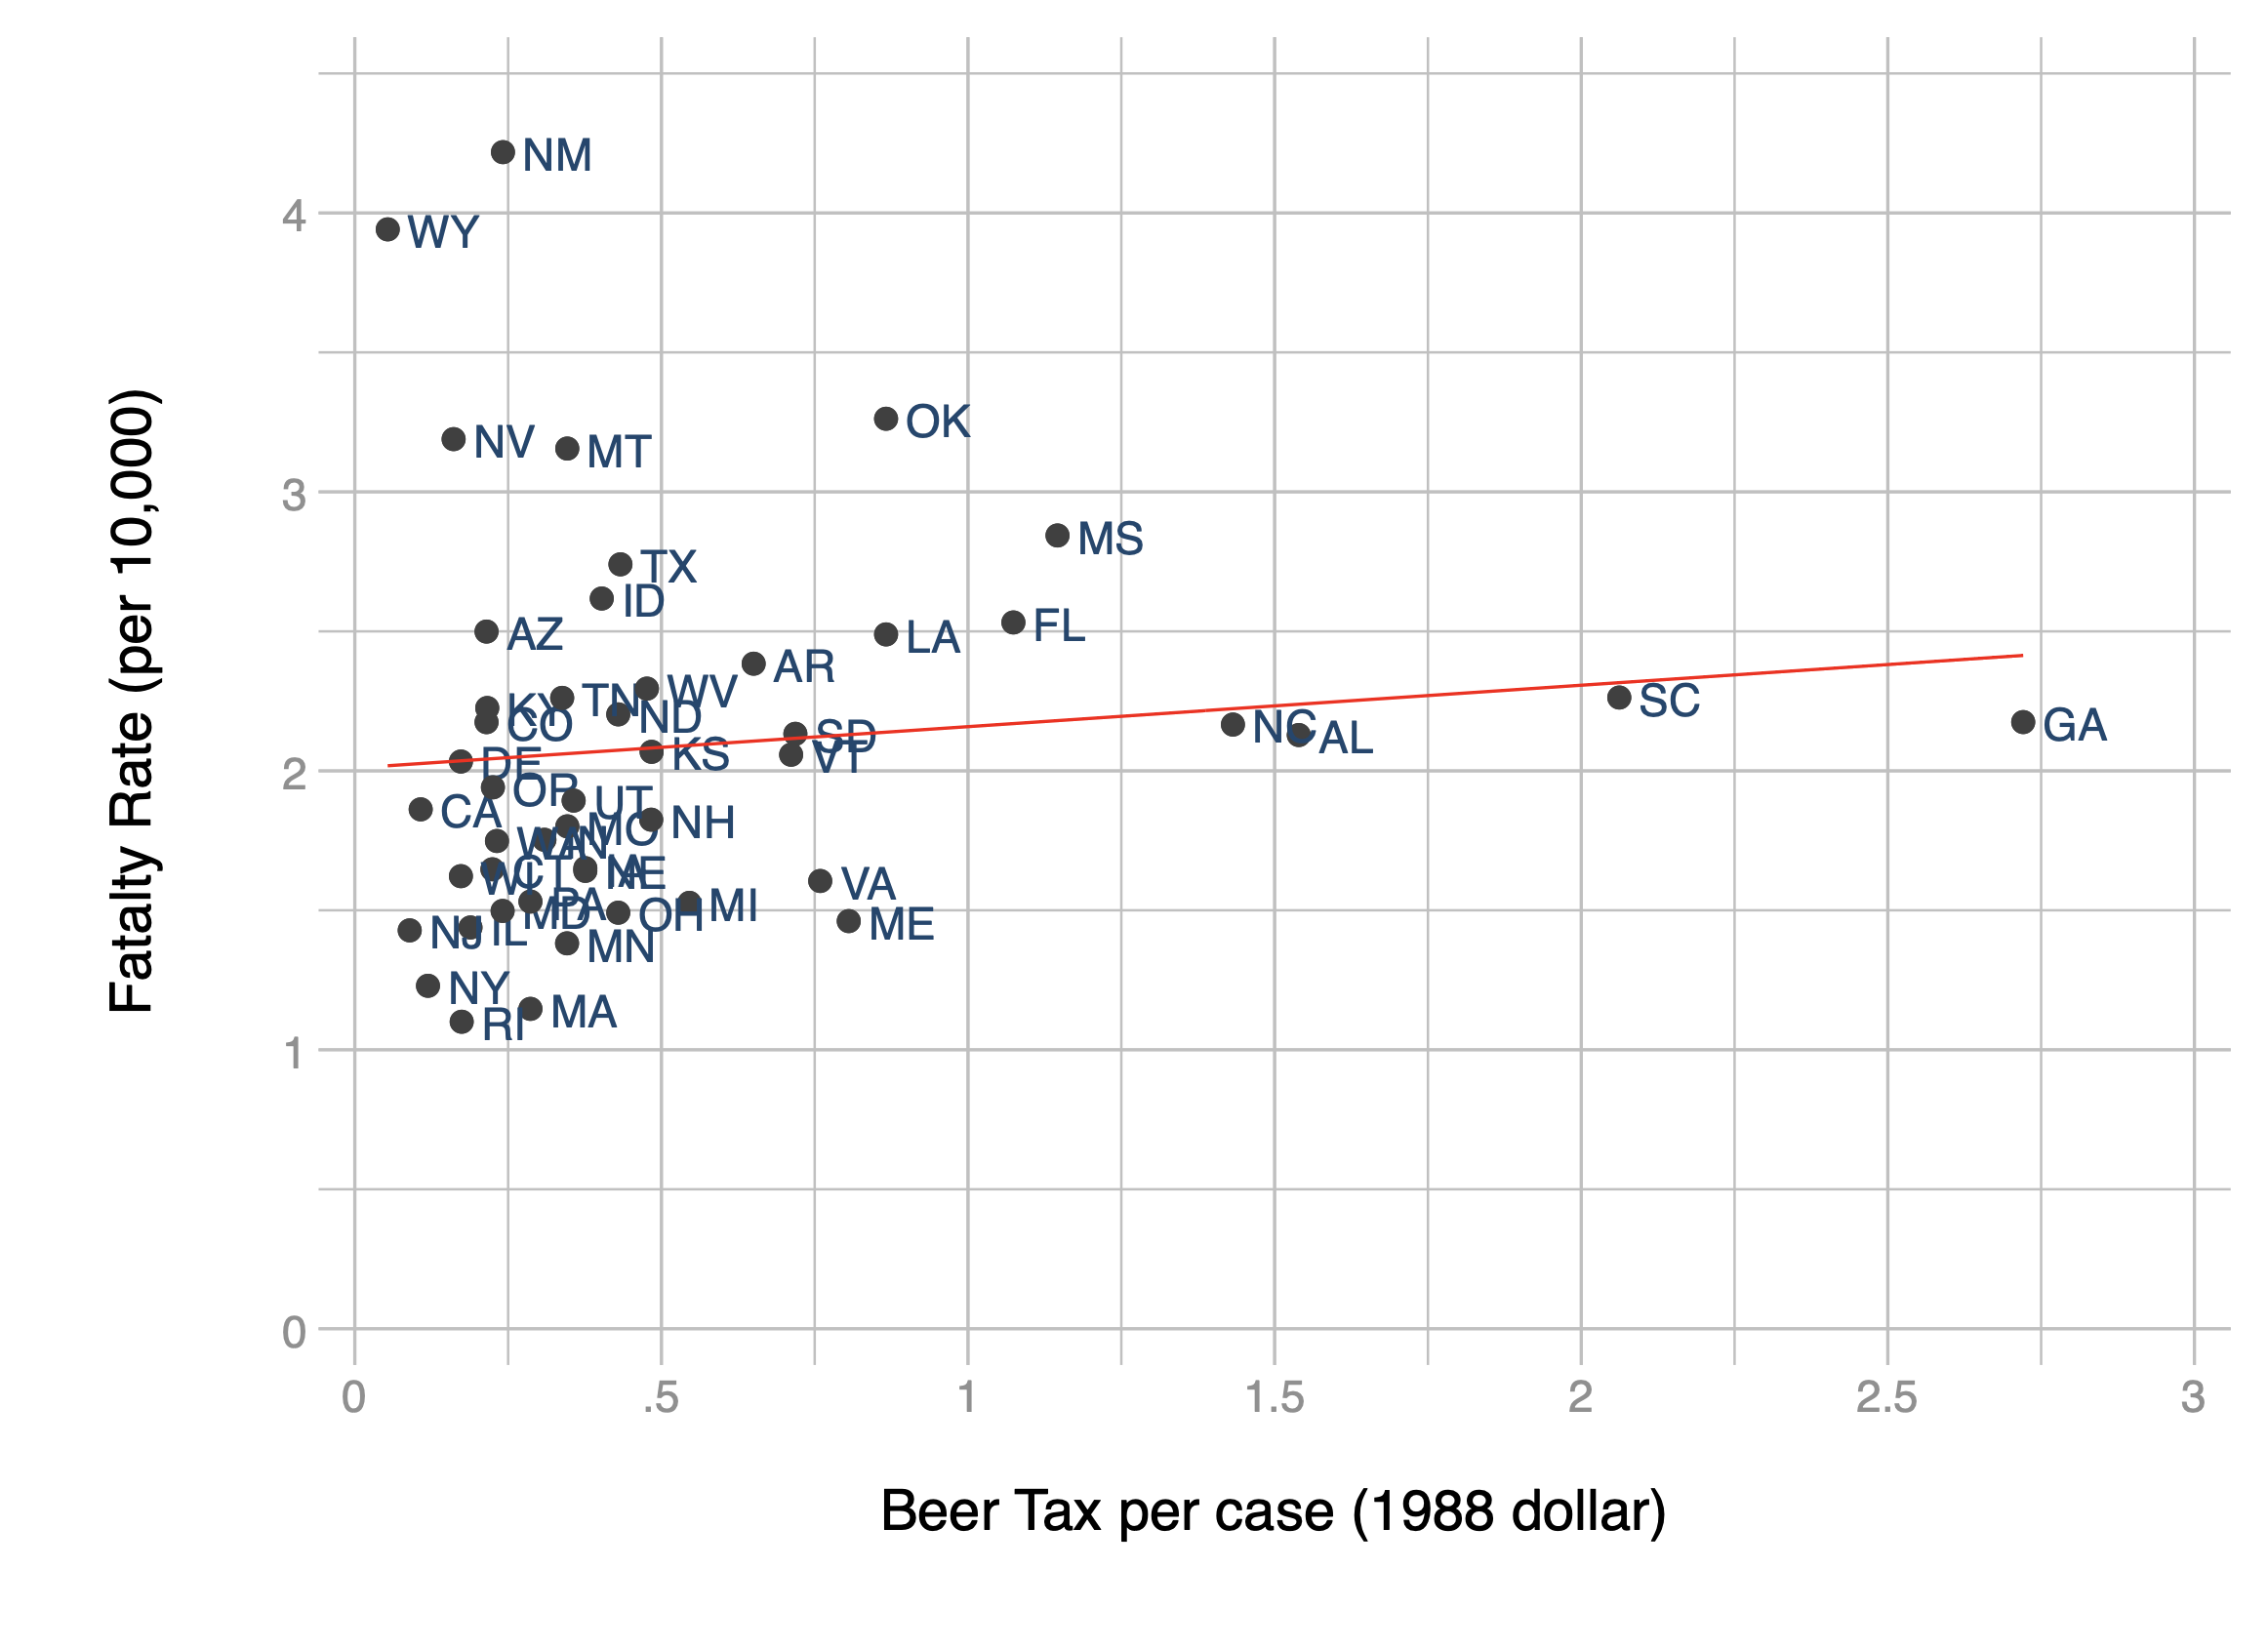
\includegraphics[width=.75\linewidth]{images/beertax1982.png}
\end{figure}
\end{frame}

\begin{frame}{Traffic Fatalities vs. Beer Tax --- 1983}
\begin{figure}
  \centering
         \vspace{-1mm}
         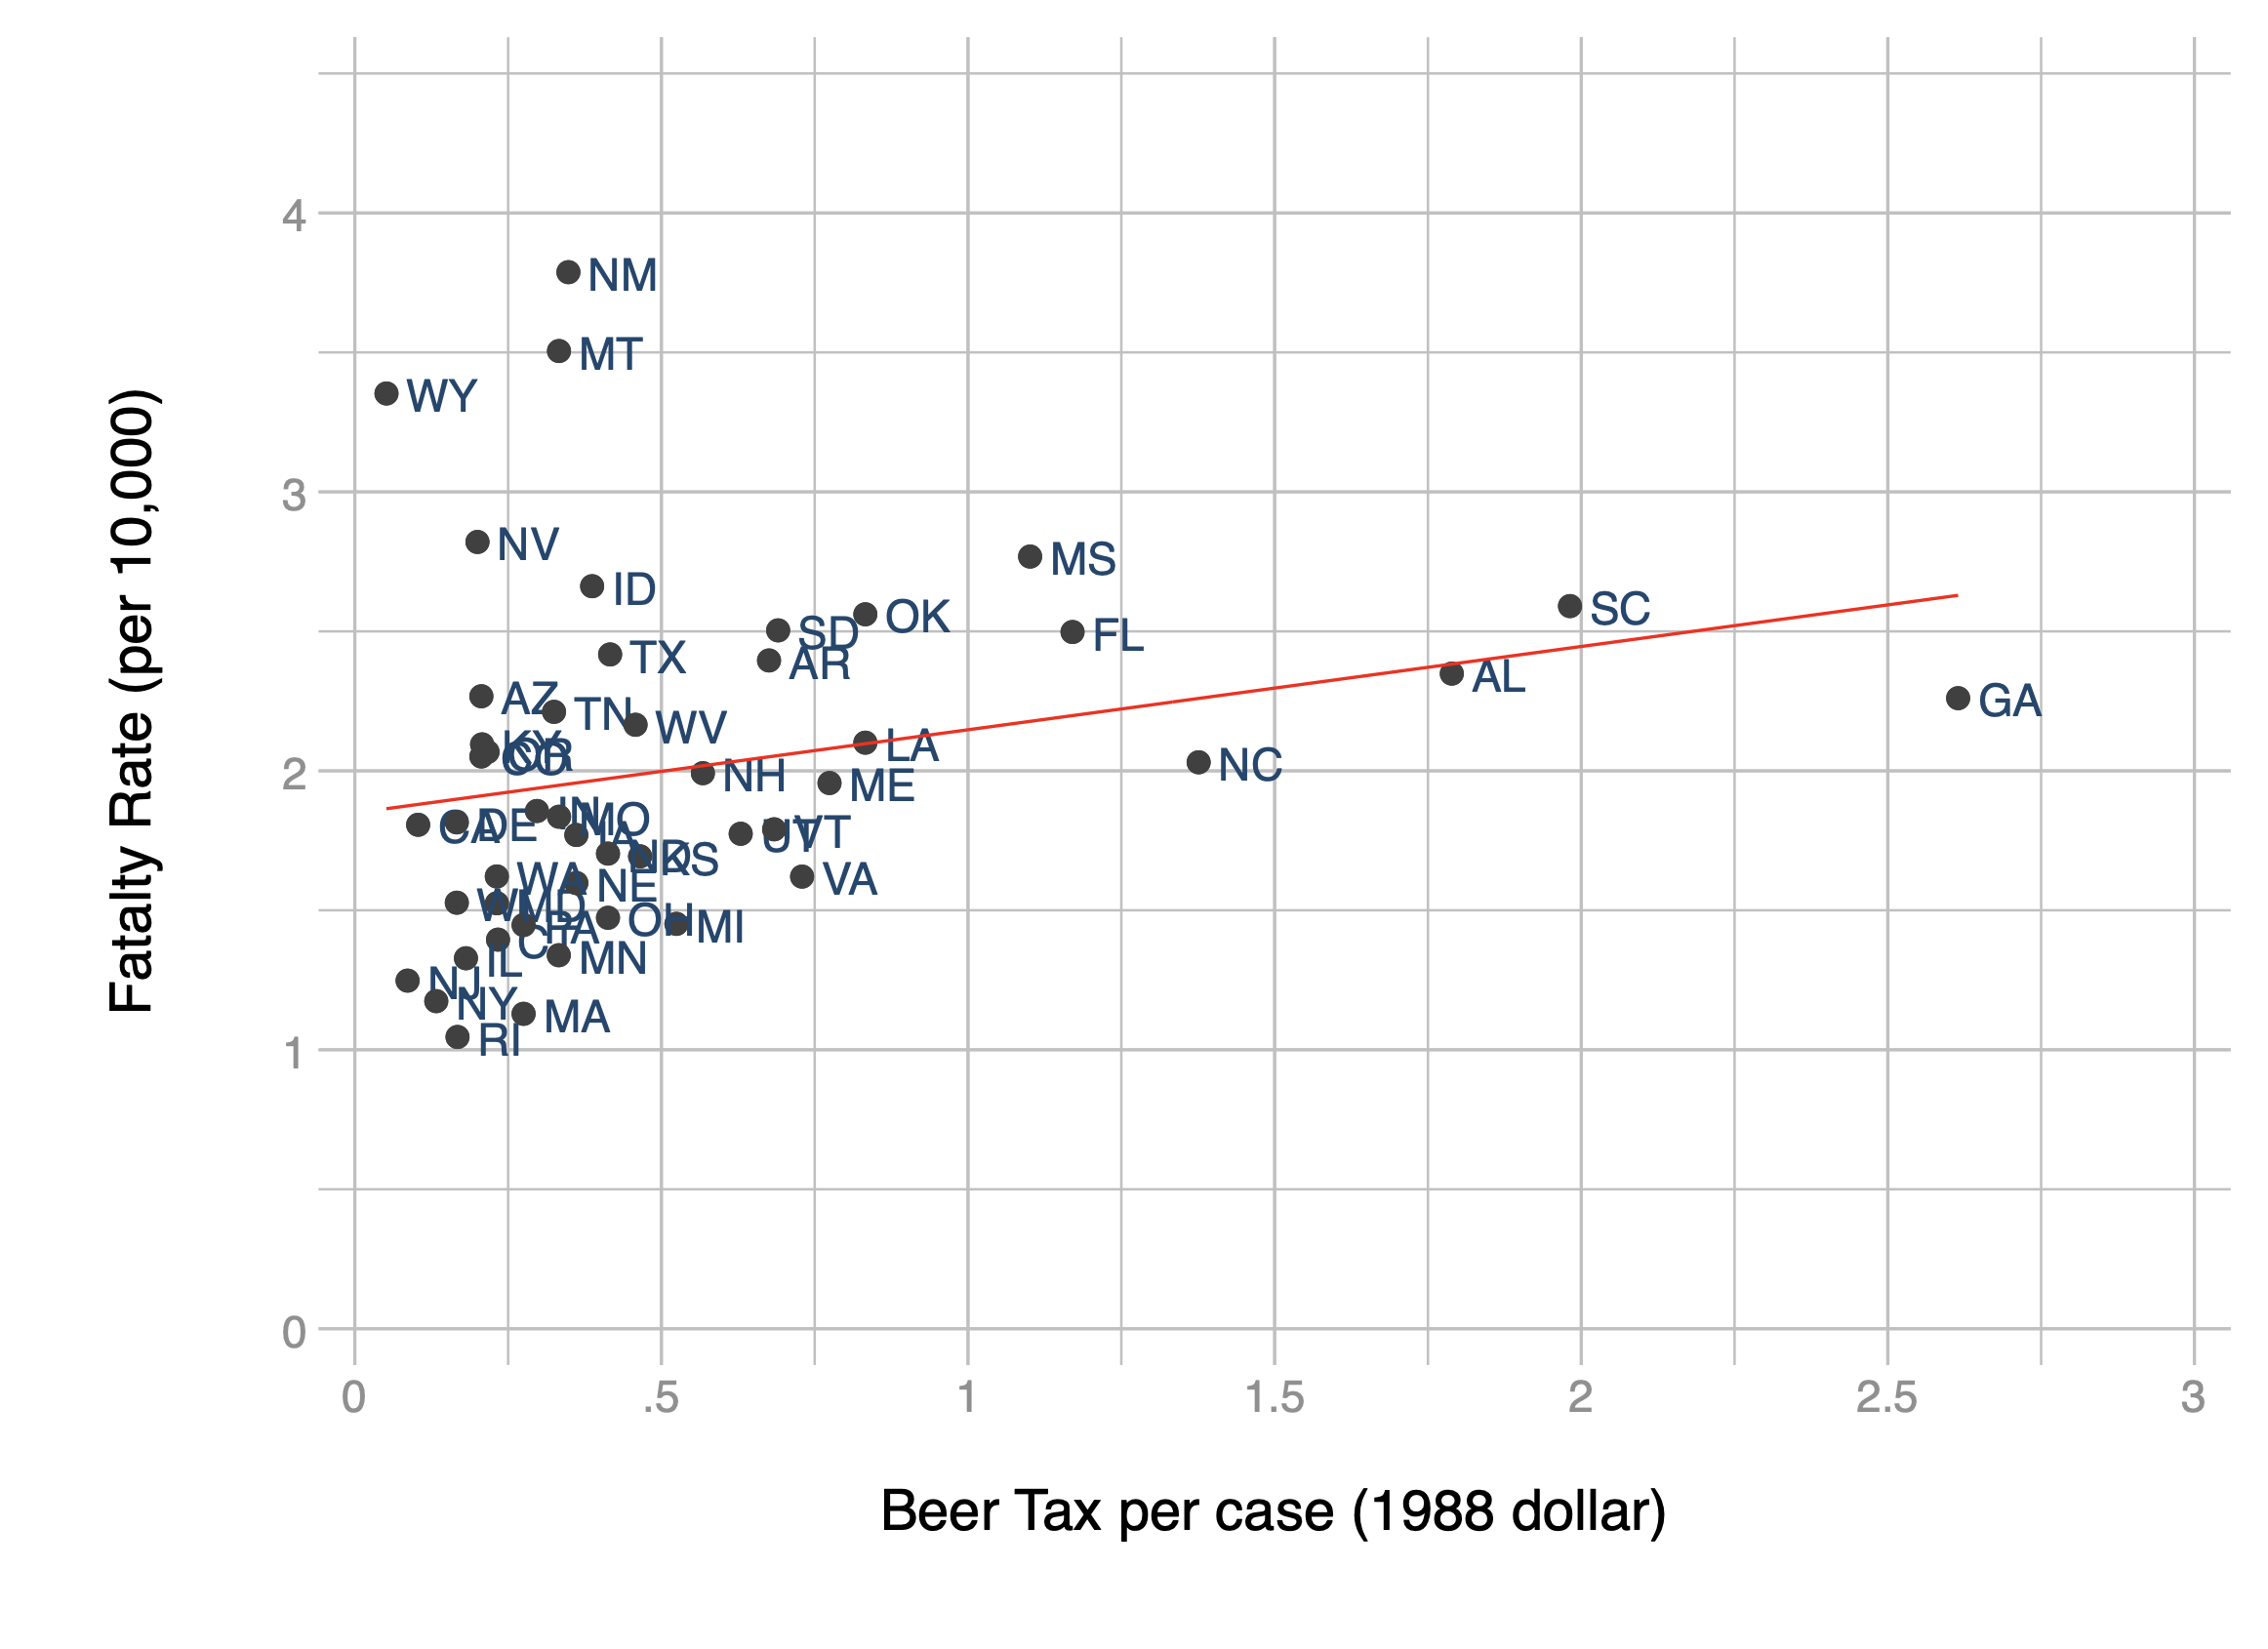
\includegraphics[width=.75\linewidth]{images/beertax1983.png}
\end{figure}
\end{frame}

\begin{frame}{Traffic Fatalities vs. Beer Tax --- 1984}
\begin{figure}
  \centering
         \vspace{-1mm}
         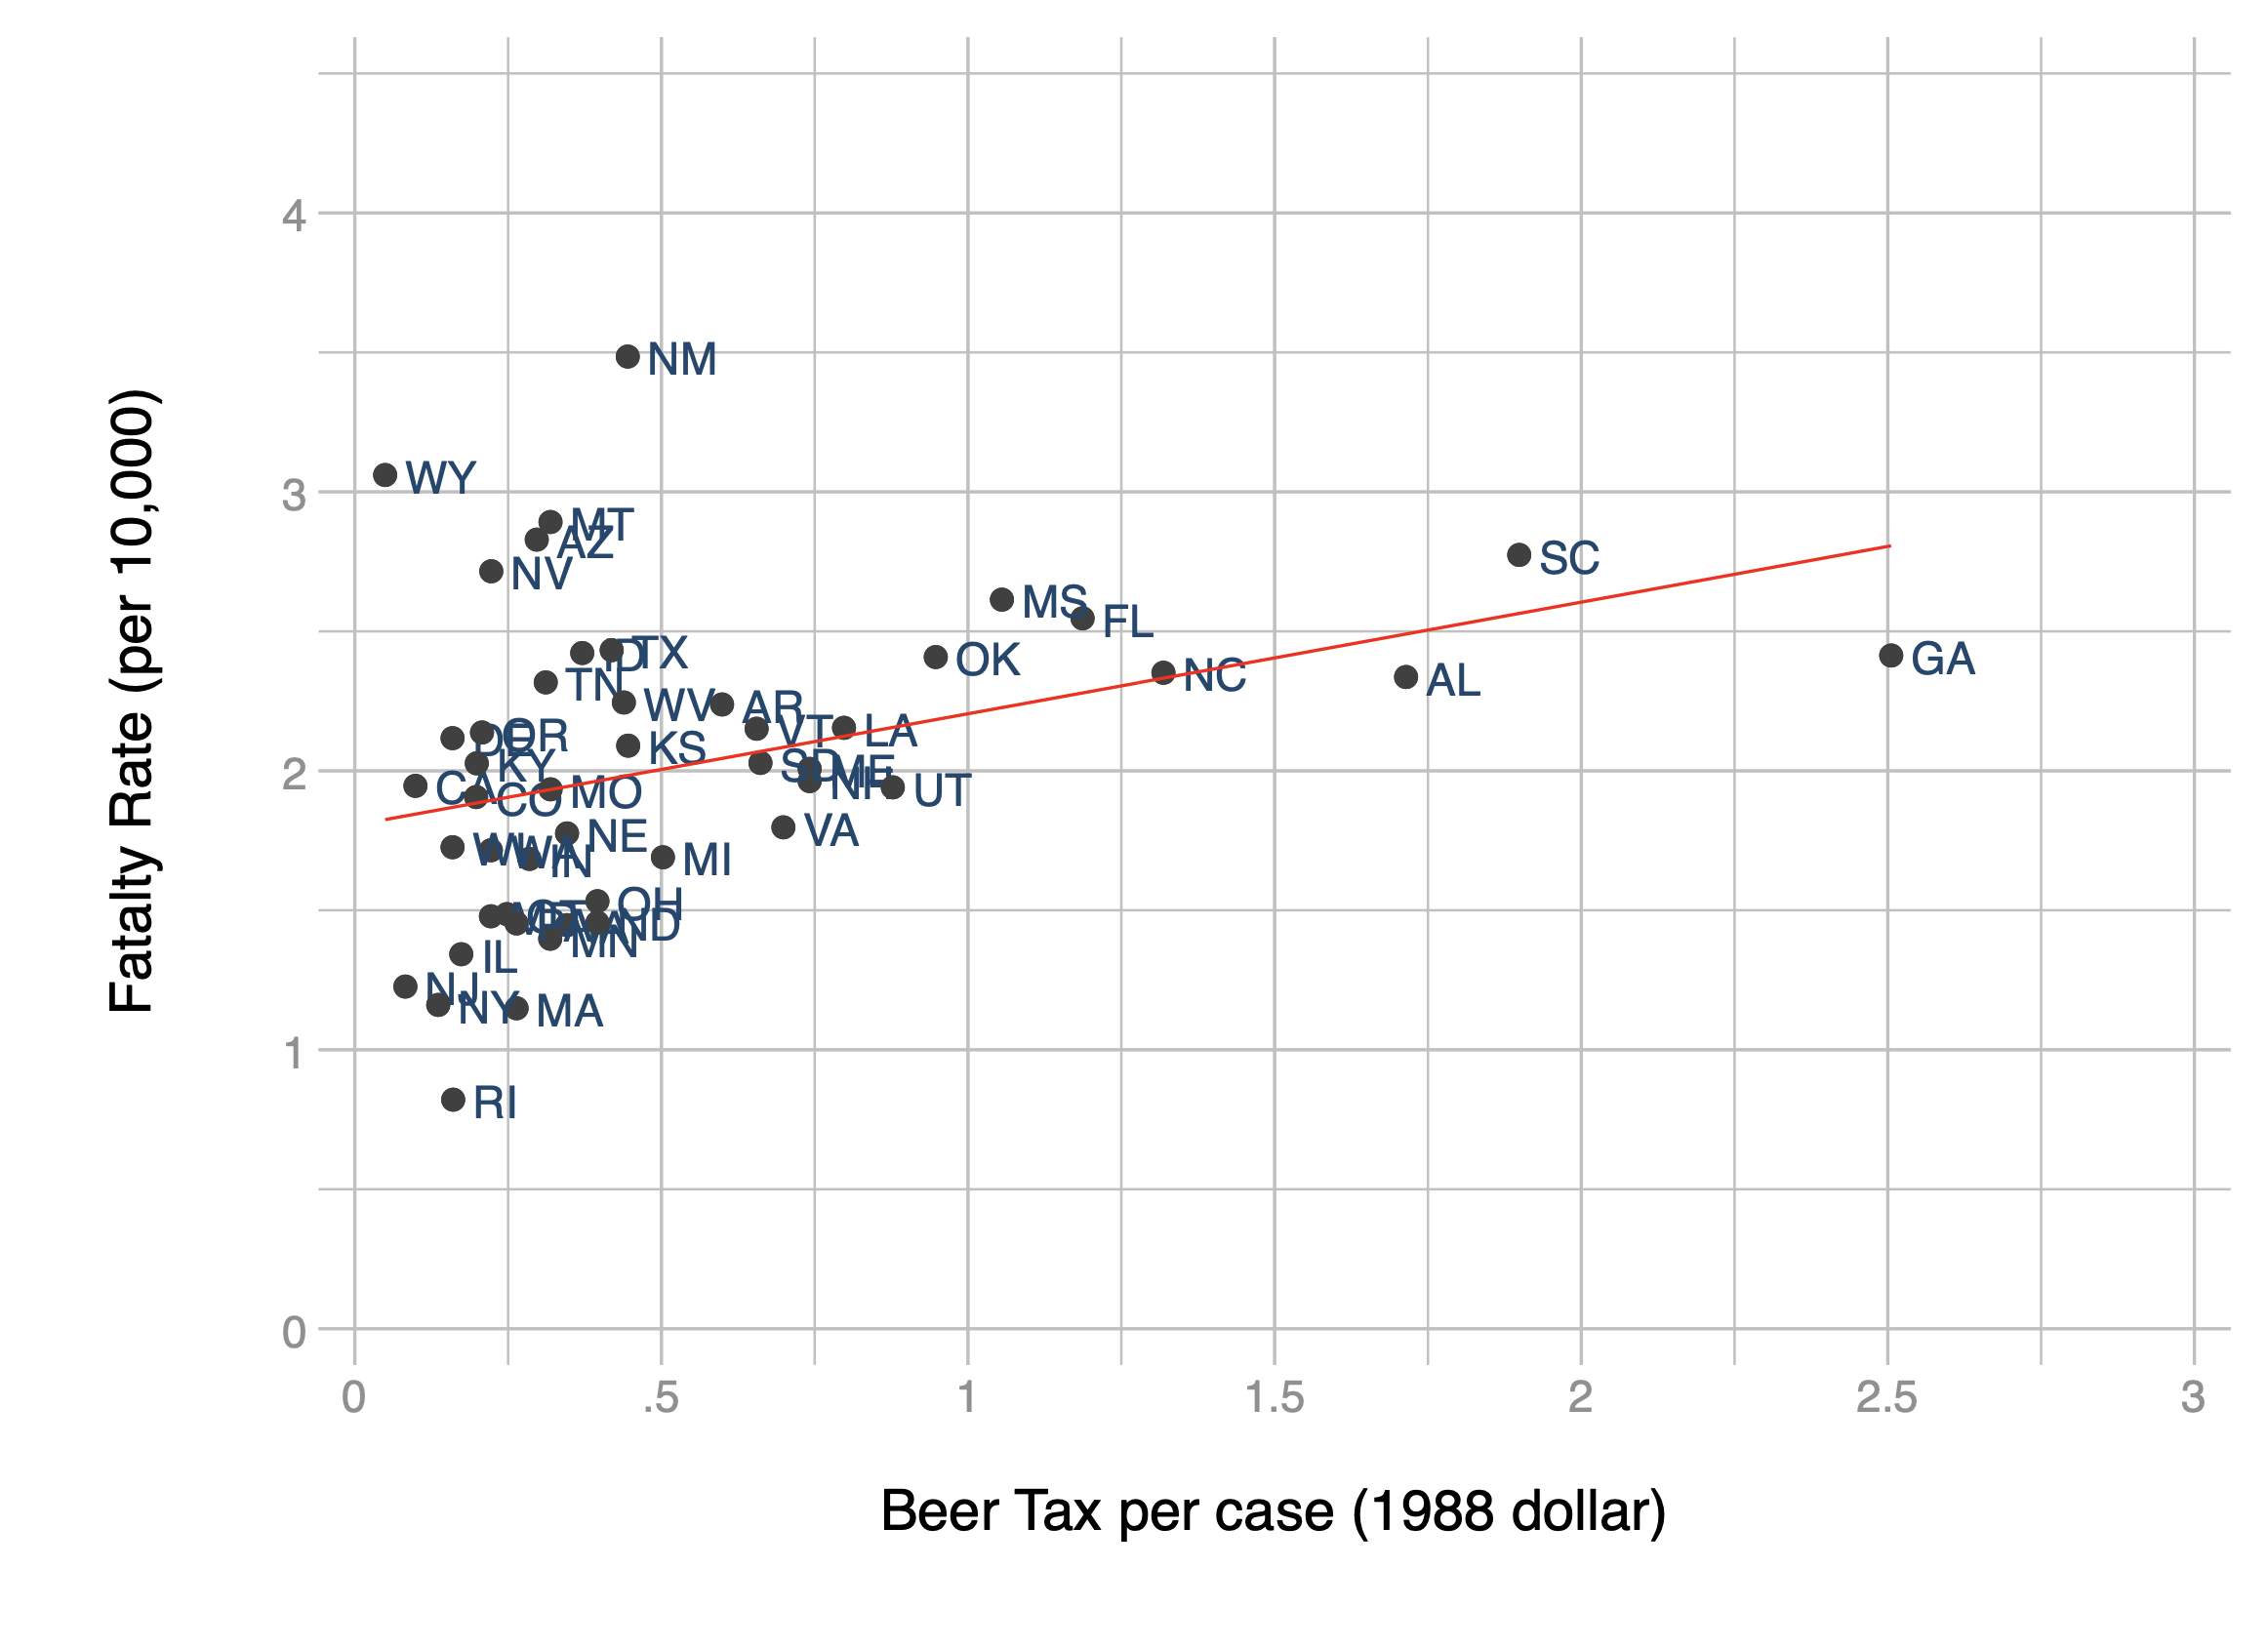
\includegraphics[width=.75\linewidth]{images/beertax1984.png}
\end{figure}
\end{frame}

\begin{frame}{Traffic Fatalities vs. Beer Tax --- 1985}
\begin{figure}
  \centering
         \vspace{-1mm}
         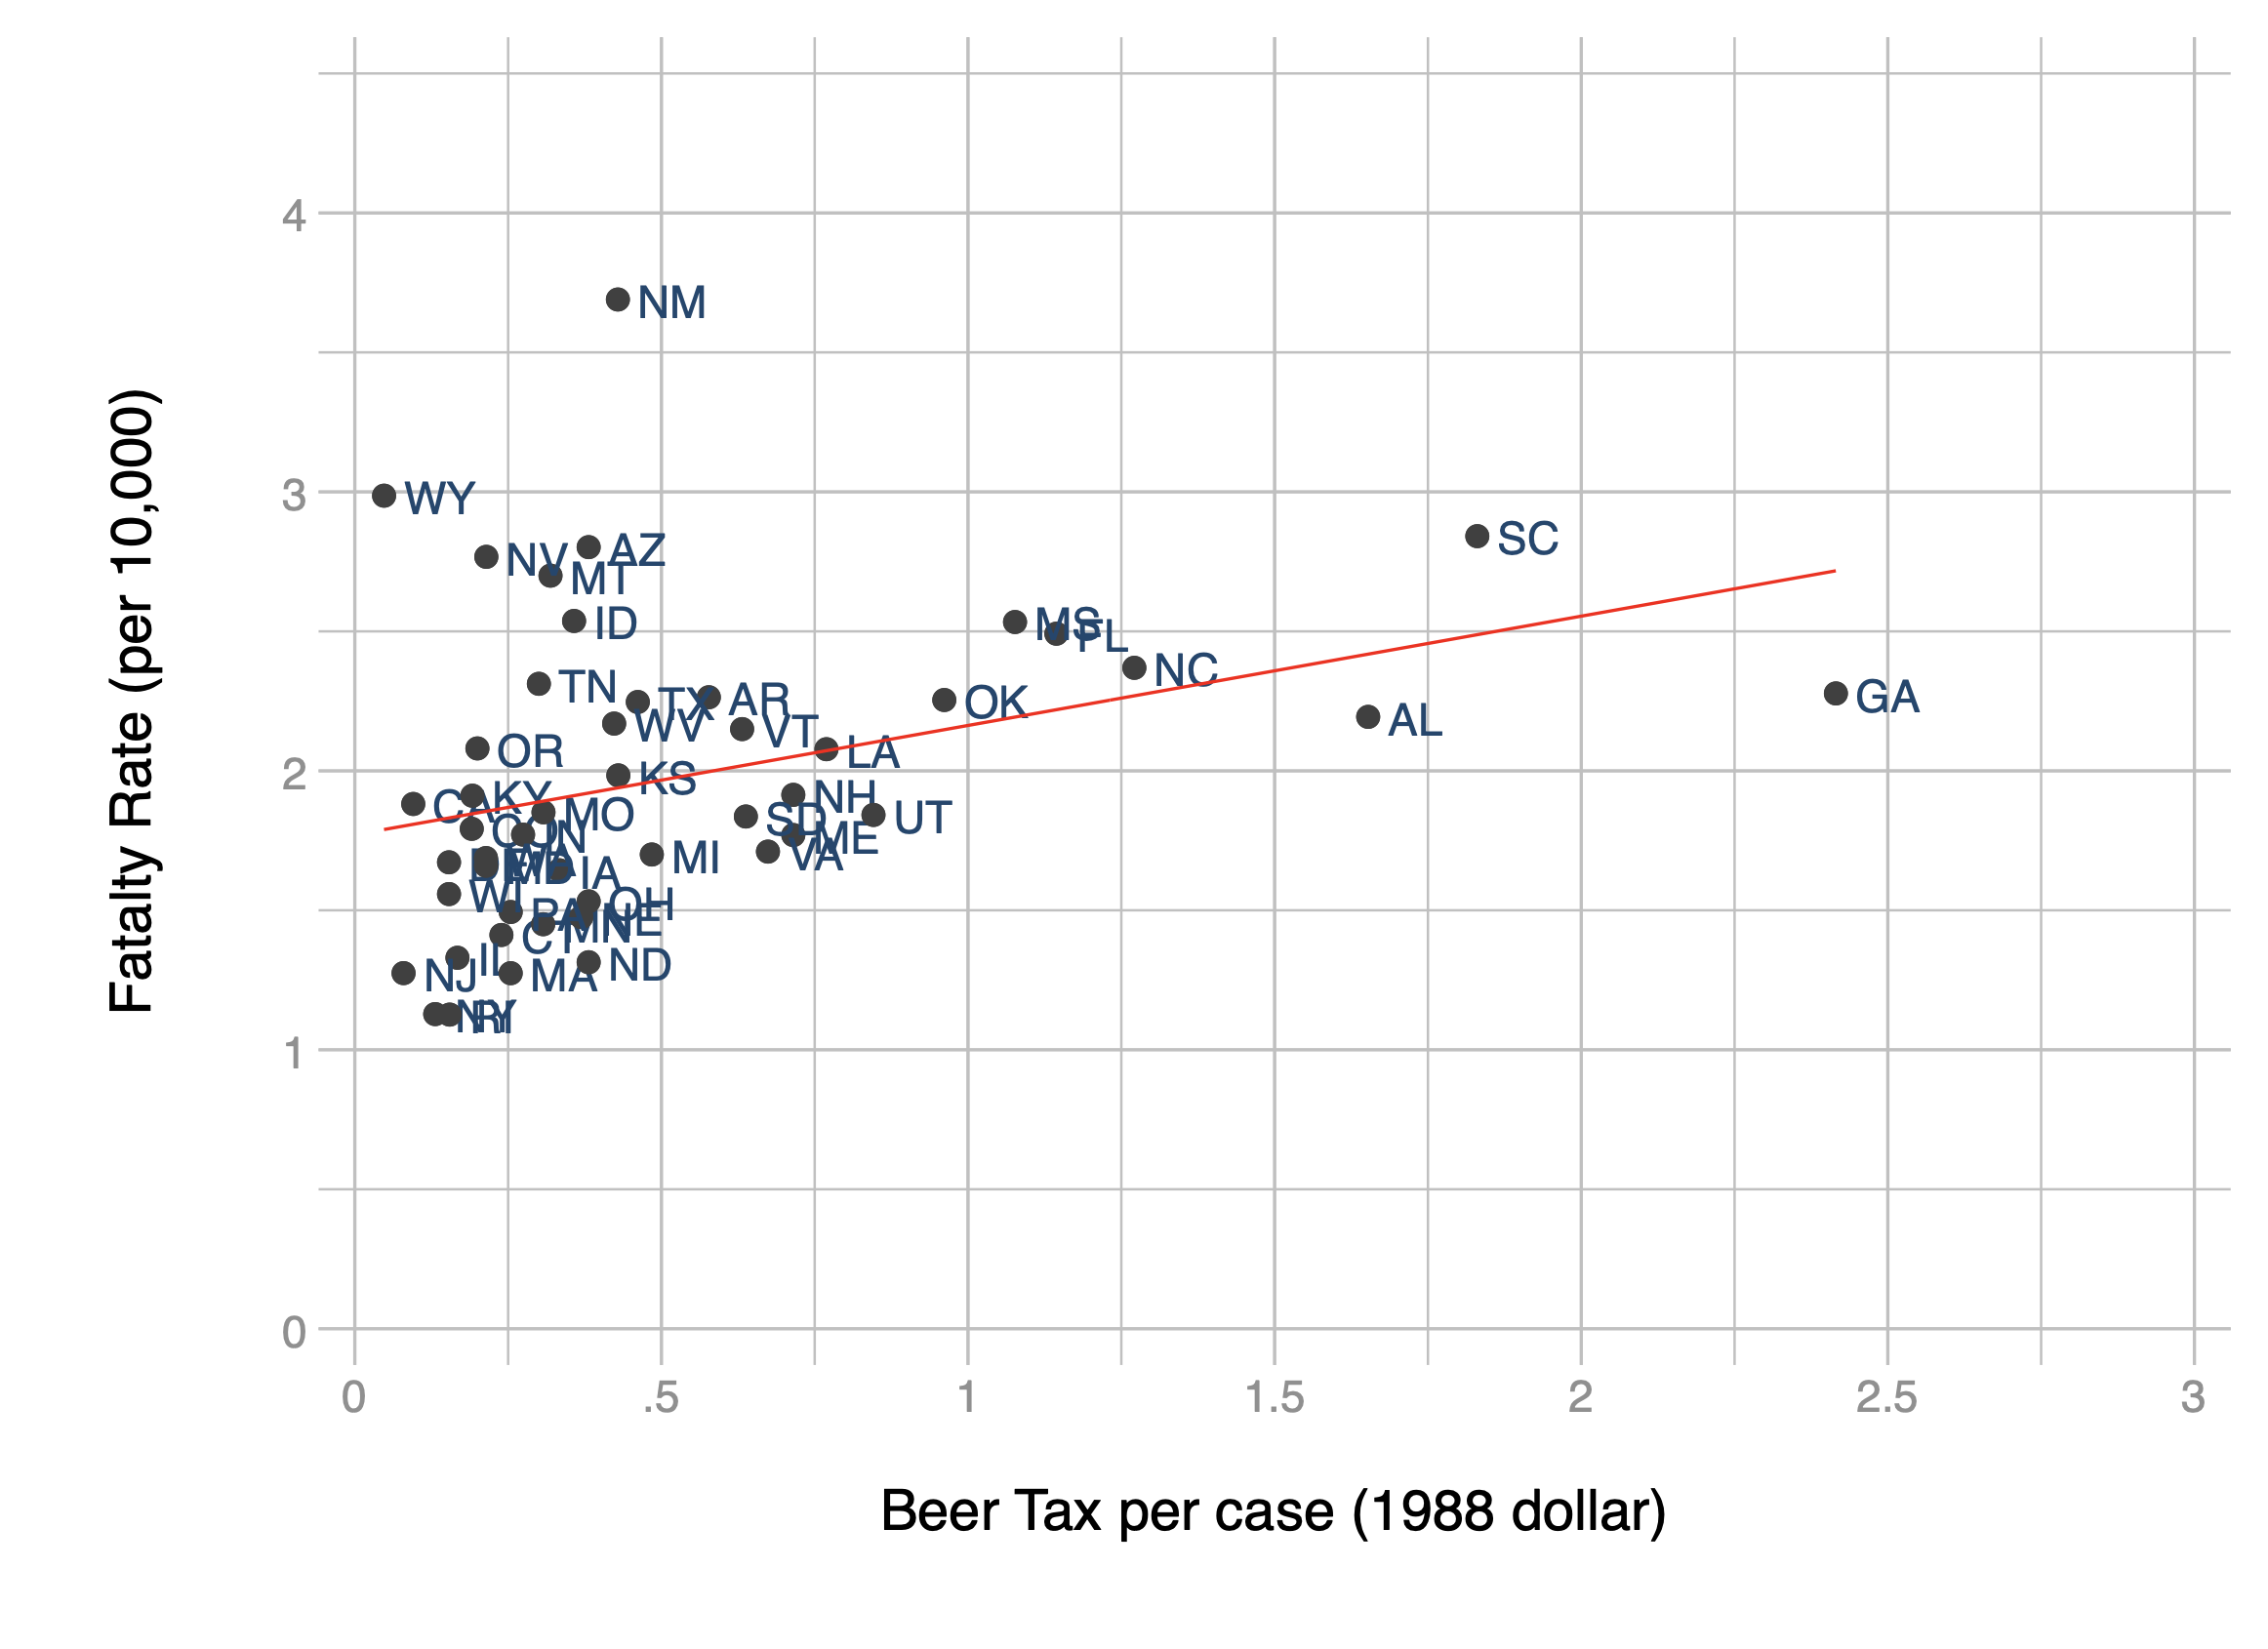
\includegraphics[width=.75\linewidth]{images/beertax1985.png}
\end{figure}
\end{frame}

\begin{frame}{Traffic Fatalities vs. Beer Tax --- 1986}
\begin{figure}
  \centering
         \vspace{-1mm}
         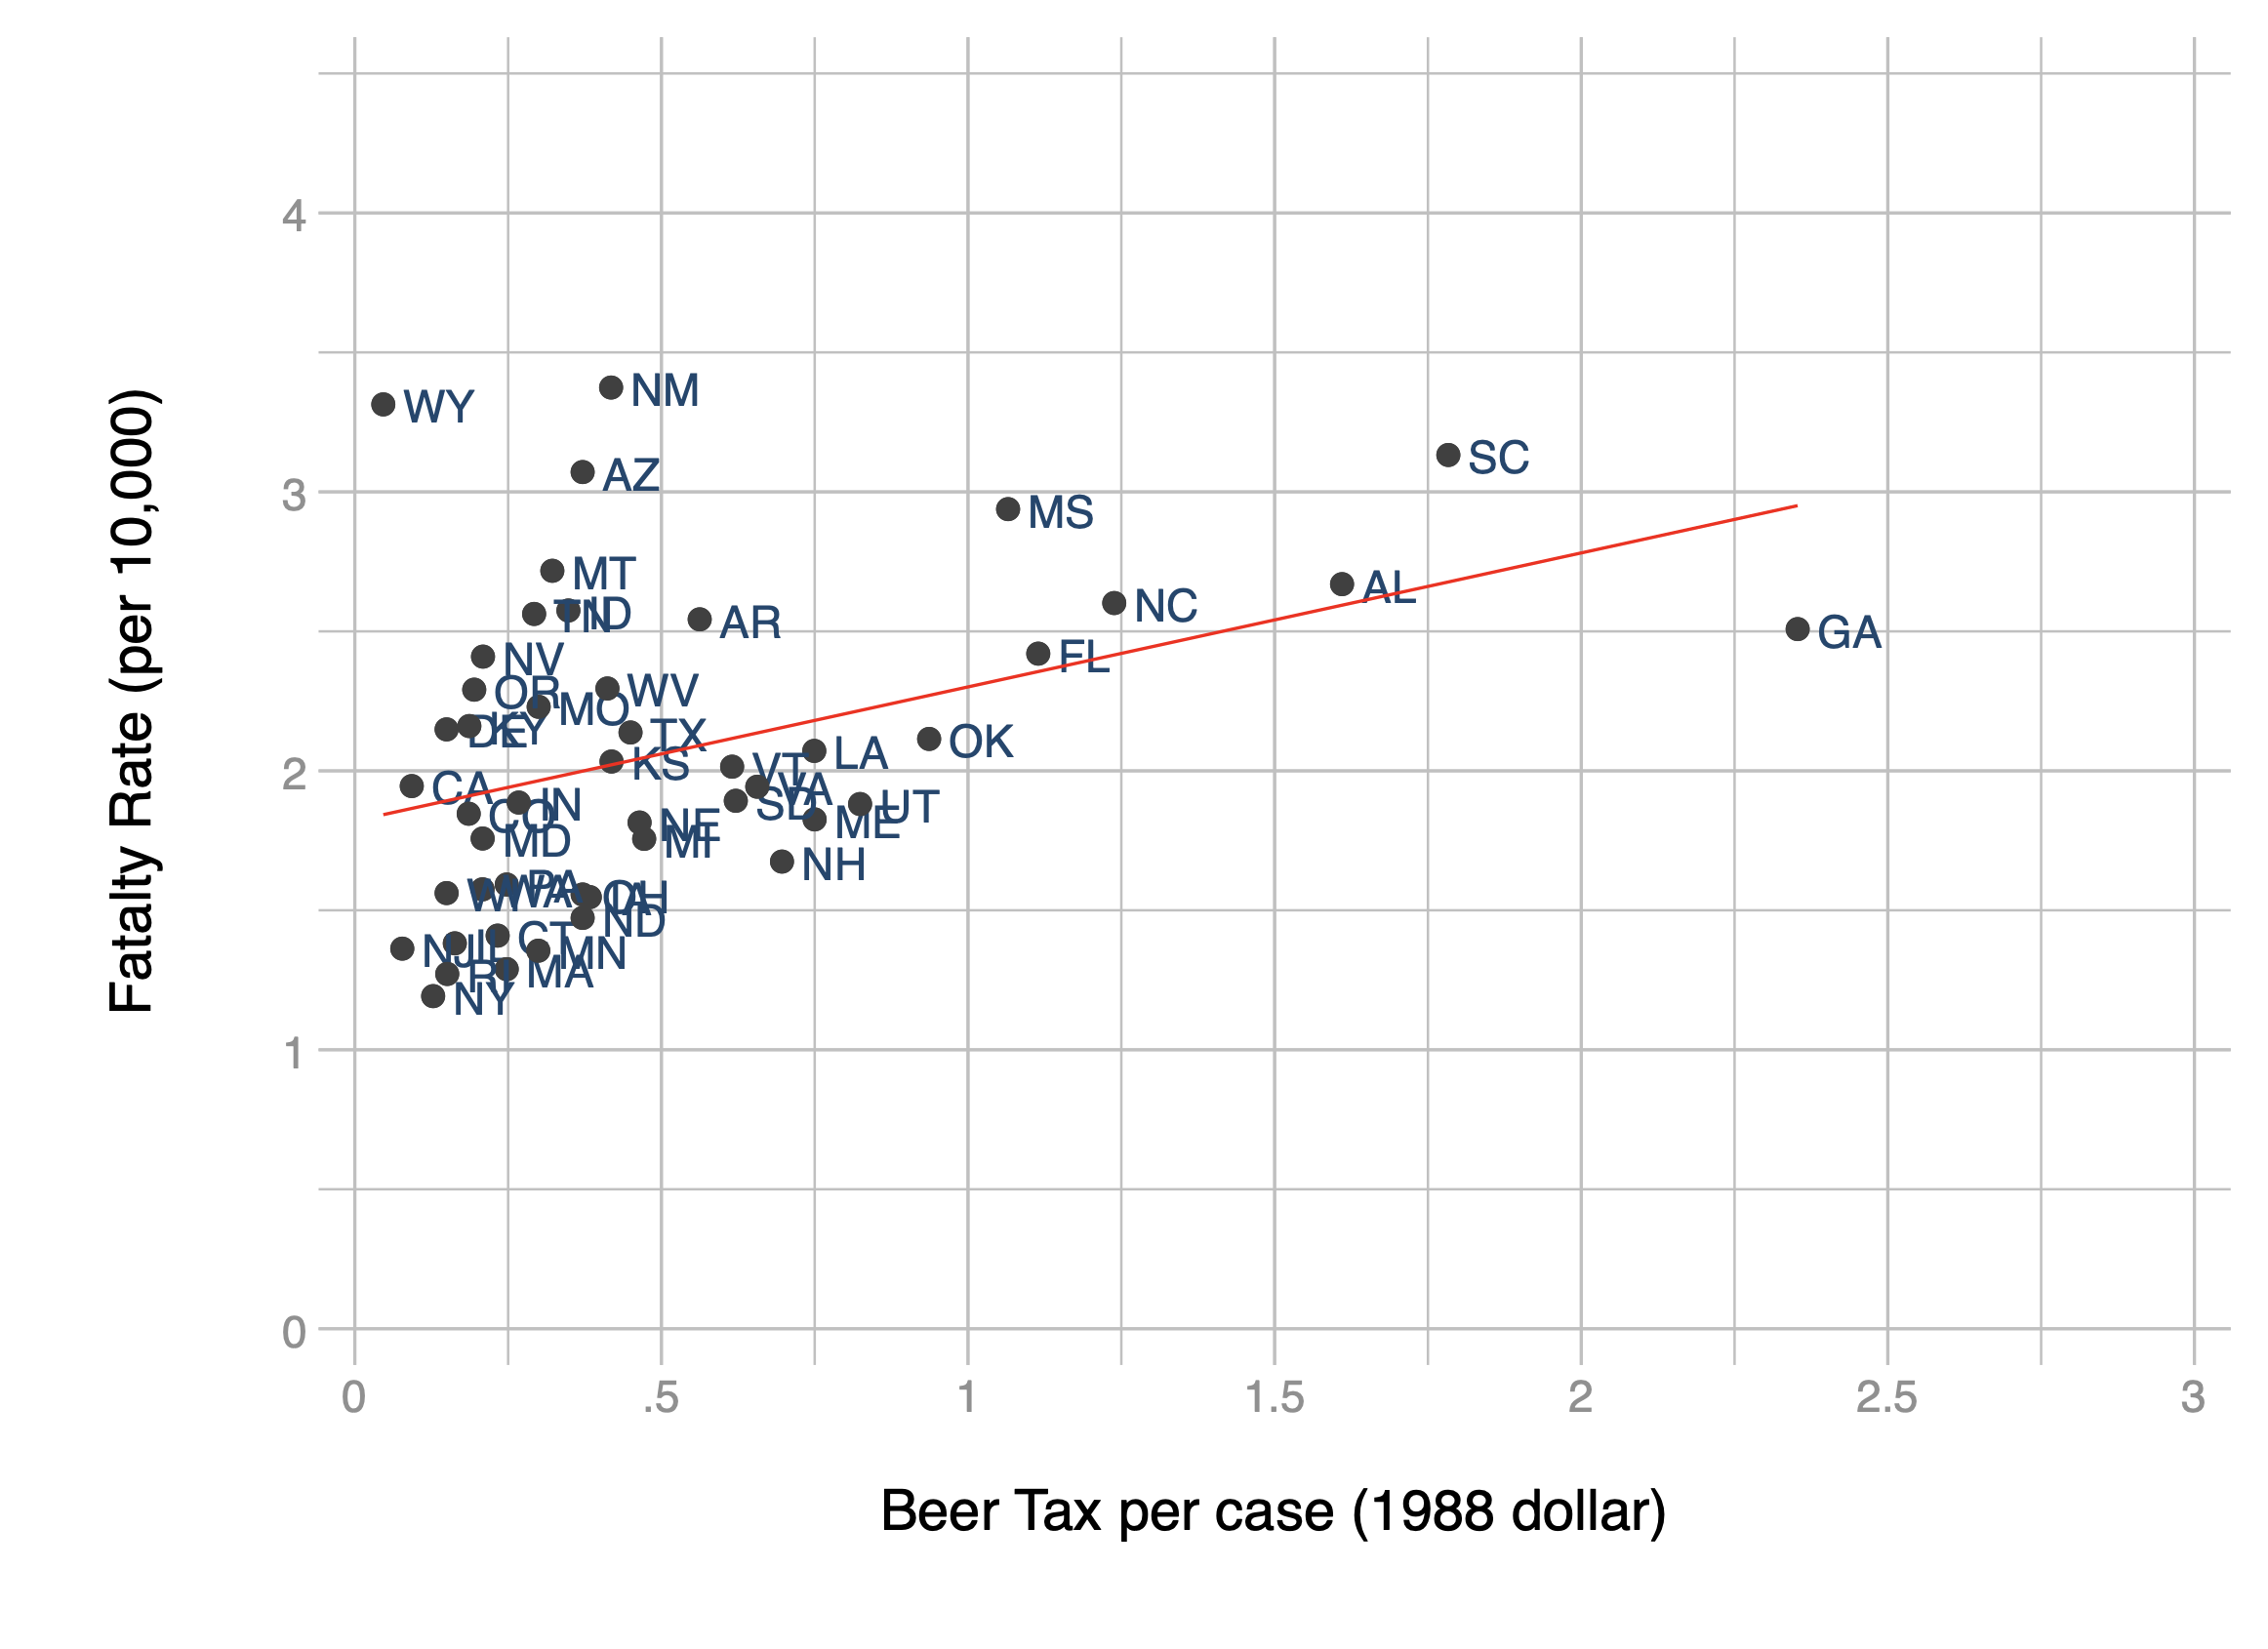
\includegraphics[width=.75\linewidth]{images/beertax1986.png}
\end{figure}
\end{frame}

\begin{frame}{Traffic Fatalities vs. Beer Tax --- 1987}
\begin{figure}
  \centering
         \vspace{-1mm}
         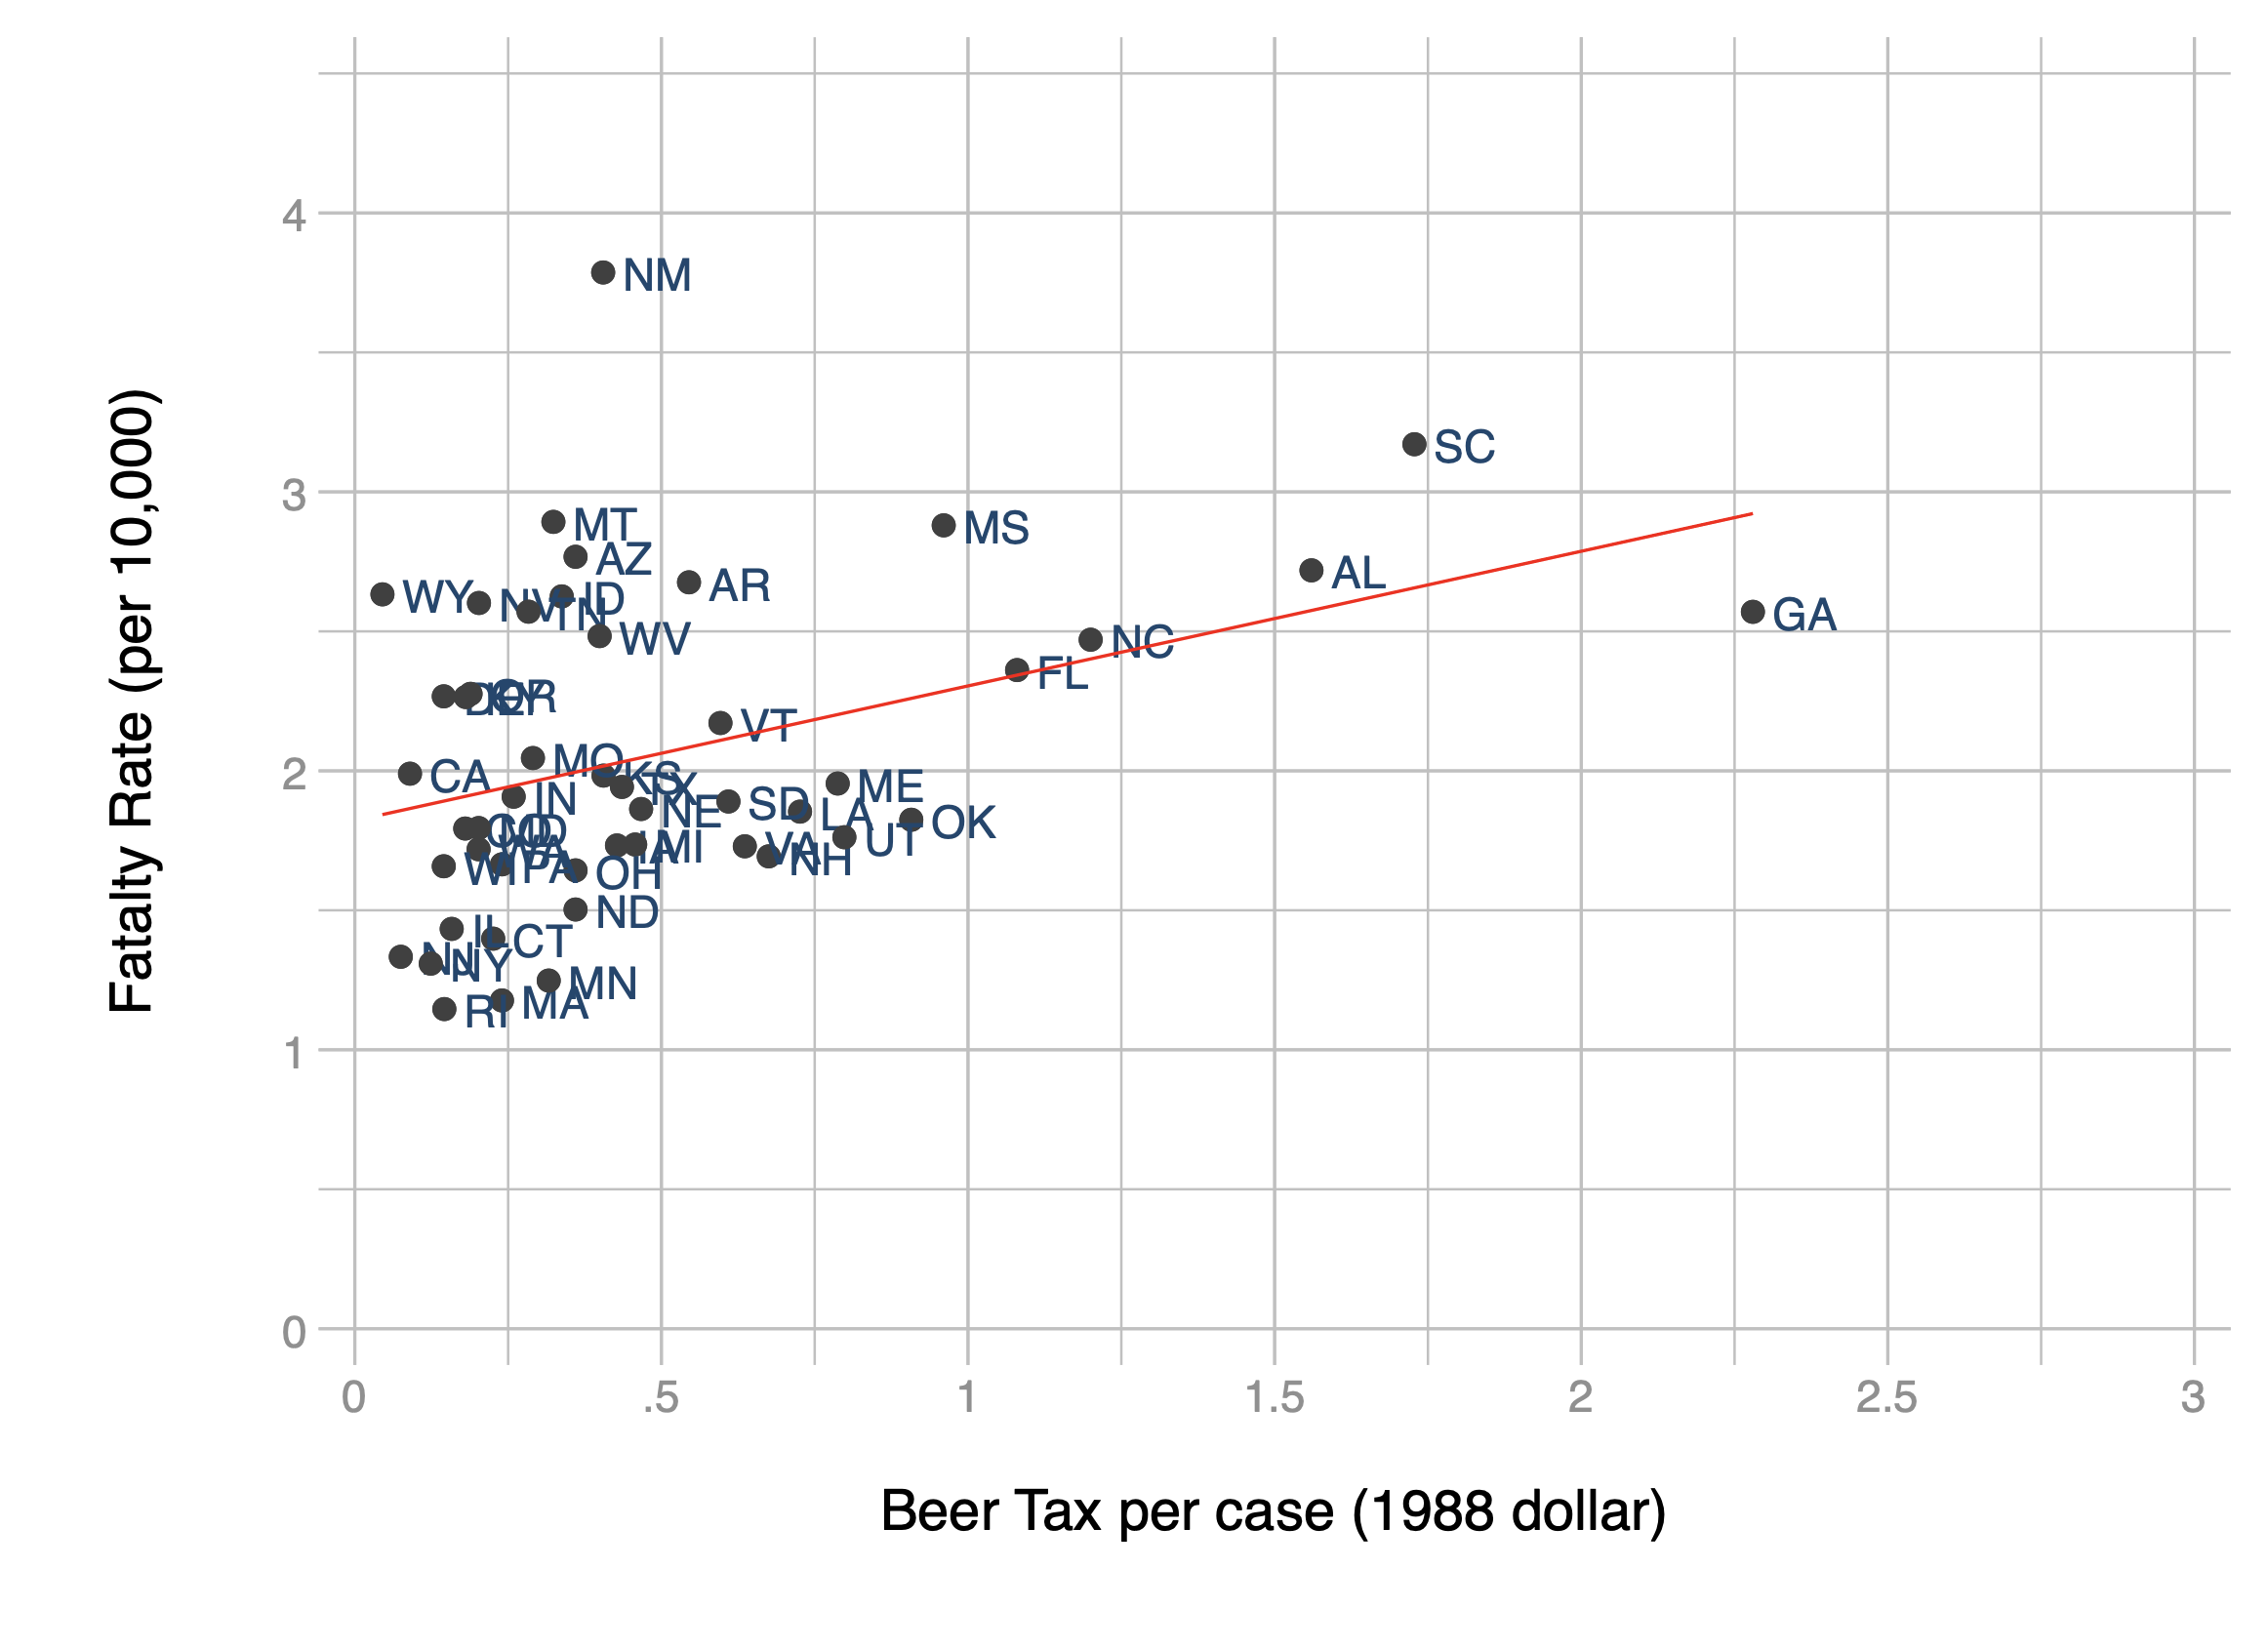
\includegraphics[width=.75\linewidth]{images/beertax1987.png}
\end{figure}
\end{frame}

\begin{frame}{Traffic Fatalities vs. Beer Tax --- 1988}
\begin{figure}
  \centering
         \vspace{-1mm}
         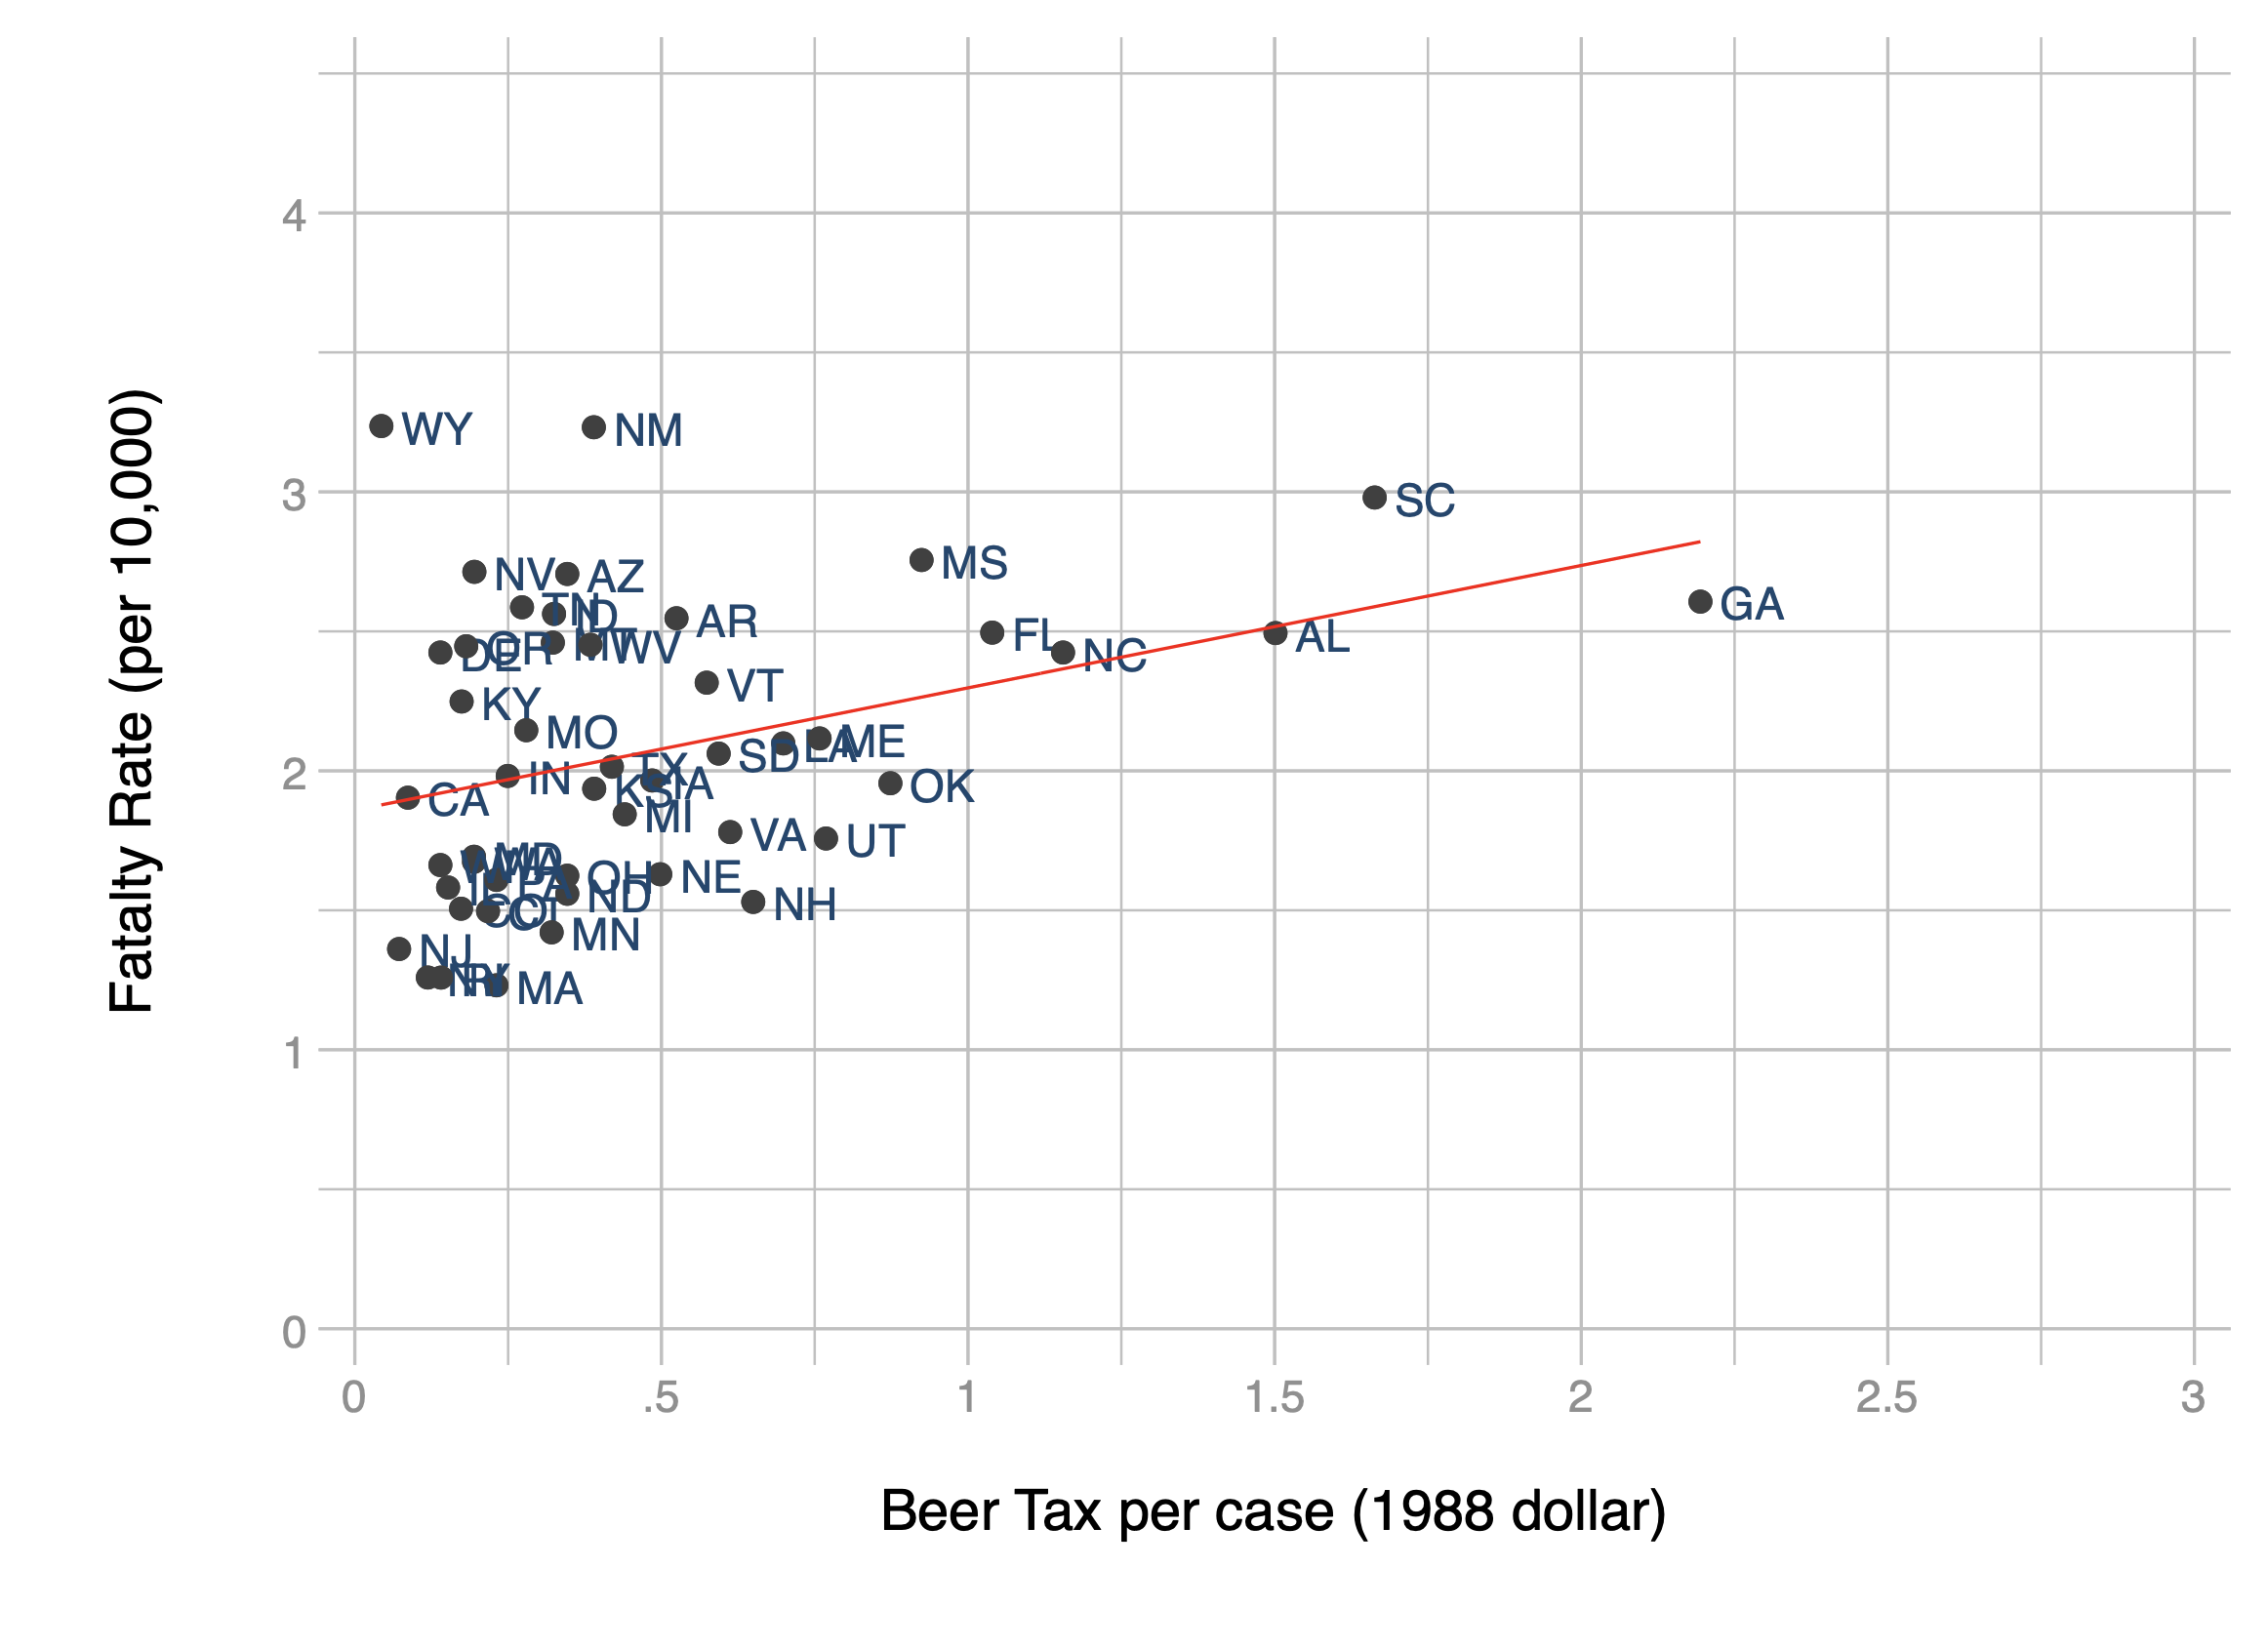
\includegraphics[width=.75\linewidth]{images/beertax1988.png}
\end{figure}
\end{frame}


\begin{frame}{Traffic Fatalities vs. Beer Tax -- First Differences}
Simple analysis of individual cross sections return weird results... Higher alcohol taxes, more traffic deaths? Arguably, omitted factors could cause omitted variable bias (which ones?)\\[1em]
Now consider the simple panel specification:
\begin{equation*}
    Fatalities_{i,t} = \beta_0 + \delta_0\mathds{1}_{1988} +\beta_1 BeerTax_{i,t} + \beta_2 Z_i + u_{i,t}
\end{equation*}
where $t\in\{1982, 1988\}$.\\[1em]
If $Z_i$ is not observed, we could run in an OVB issue. But taking the first difference eliminates the value of $Z_i$!
\begin{equation*}
    Fatalities_{i,1988}-  Fatalities_{i,1982}= \delta_0 +  \beta_1 (BeerTax_{i,1988}-BeerTax_{i,1982}) + (u_{i,1988}-u_{i,1982})
\end{equation*}\\[1em]
This “difference” equation can be estimated by OLS, even though $Z_i$ is unobserved!\\[1em]
%$\delta_0$ captures the differences in the intercepts ($\beta_0^{1982}\neq\beta_0^{1988}$!) 
\end{frame}

\begin{frame}{Traffic Fatalities vs. Beer Tax -- First Differences}
\begin{figure}
  \centering
         \vspace{-1mm}
         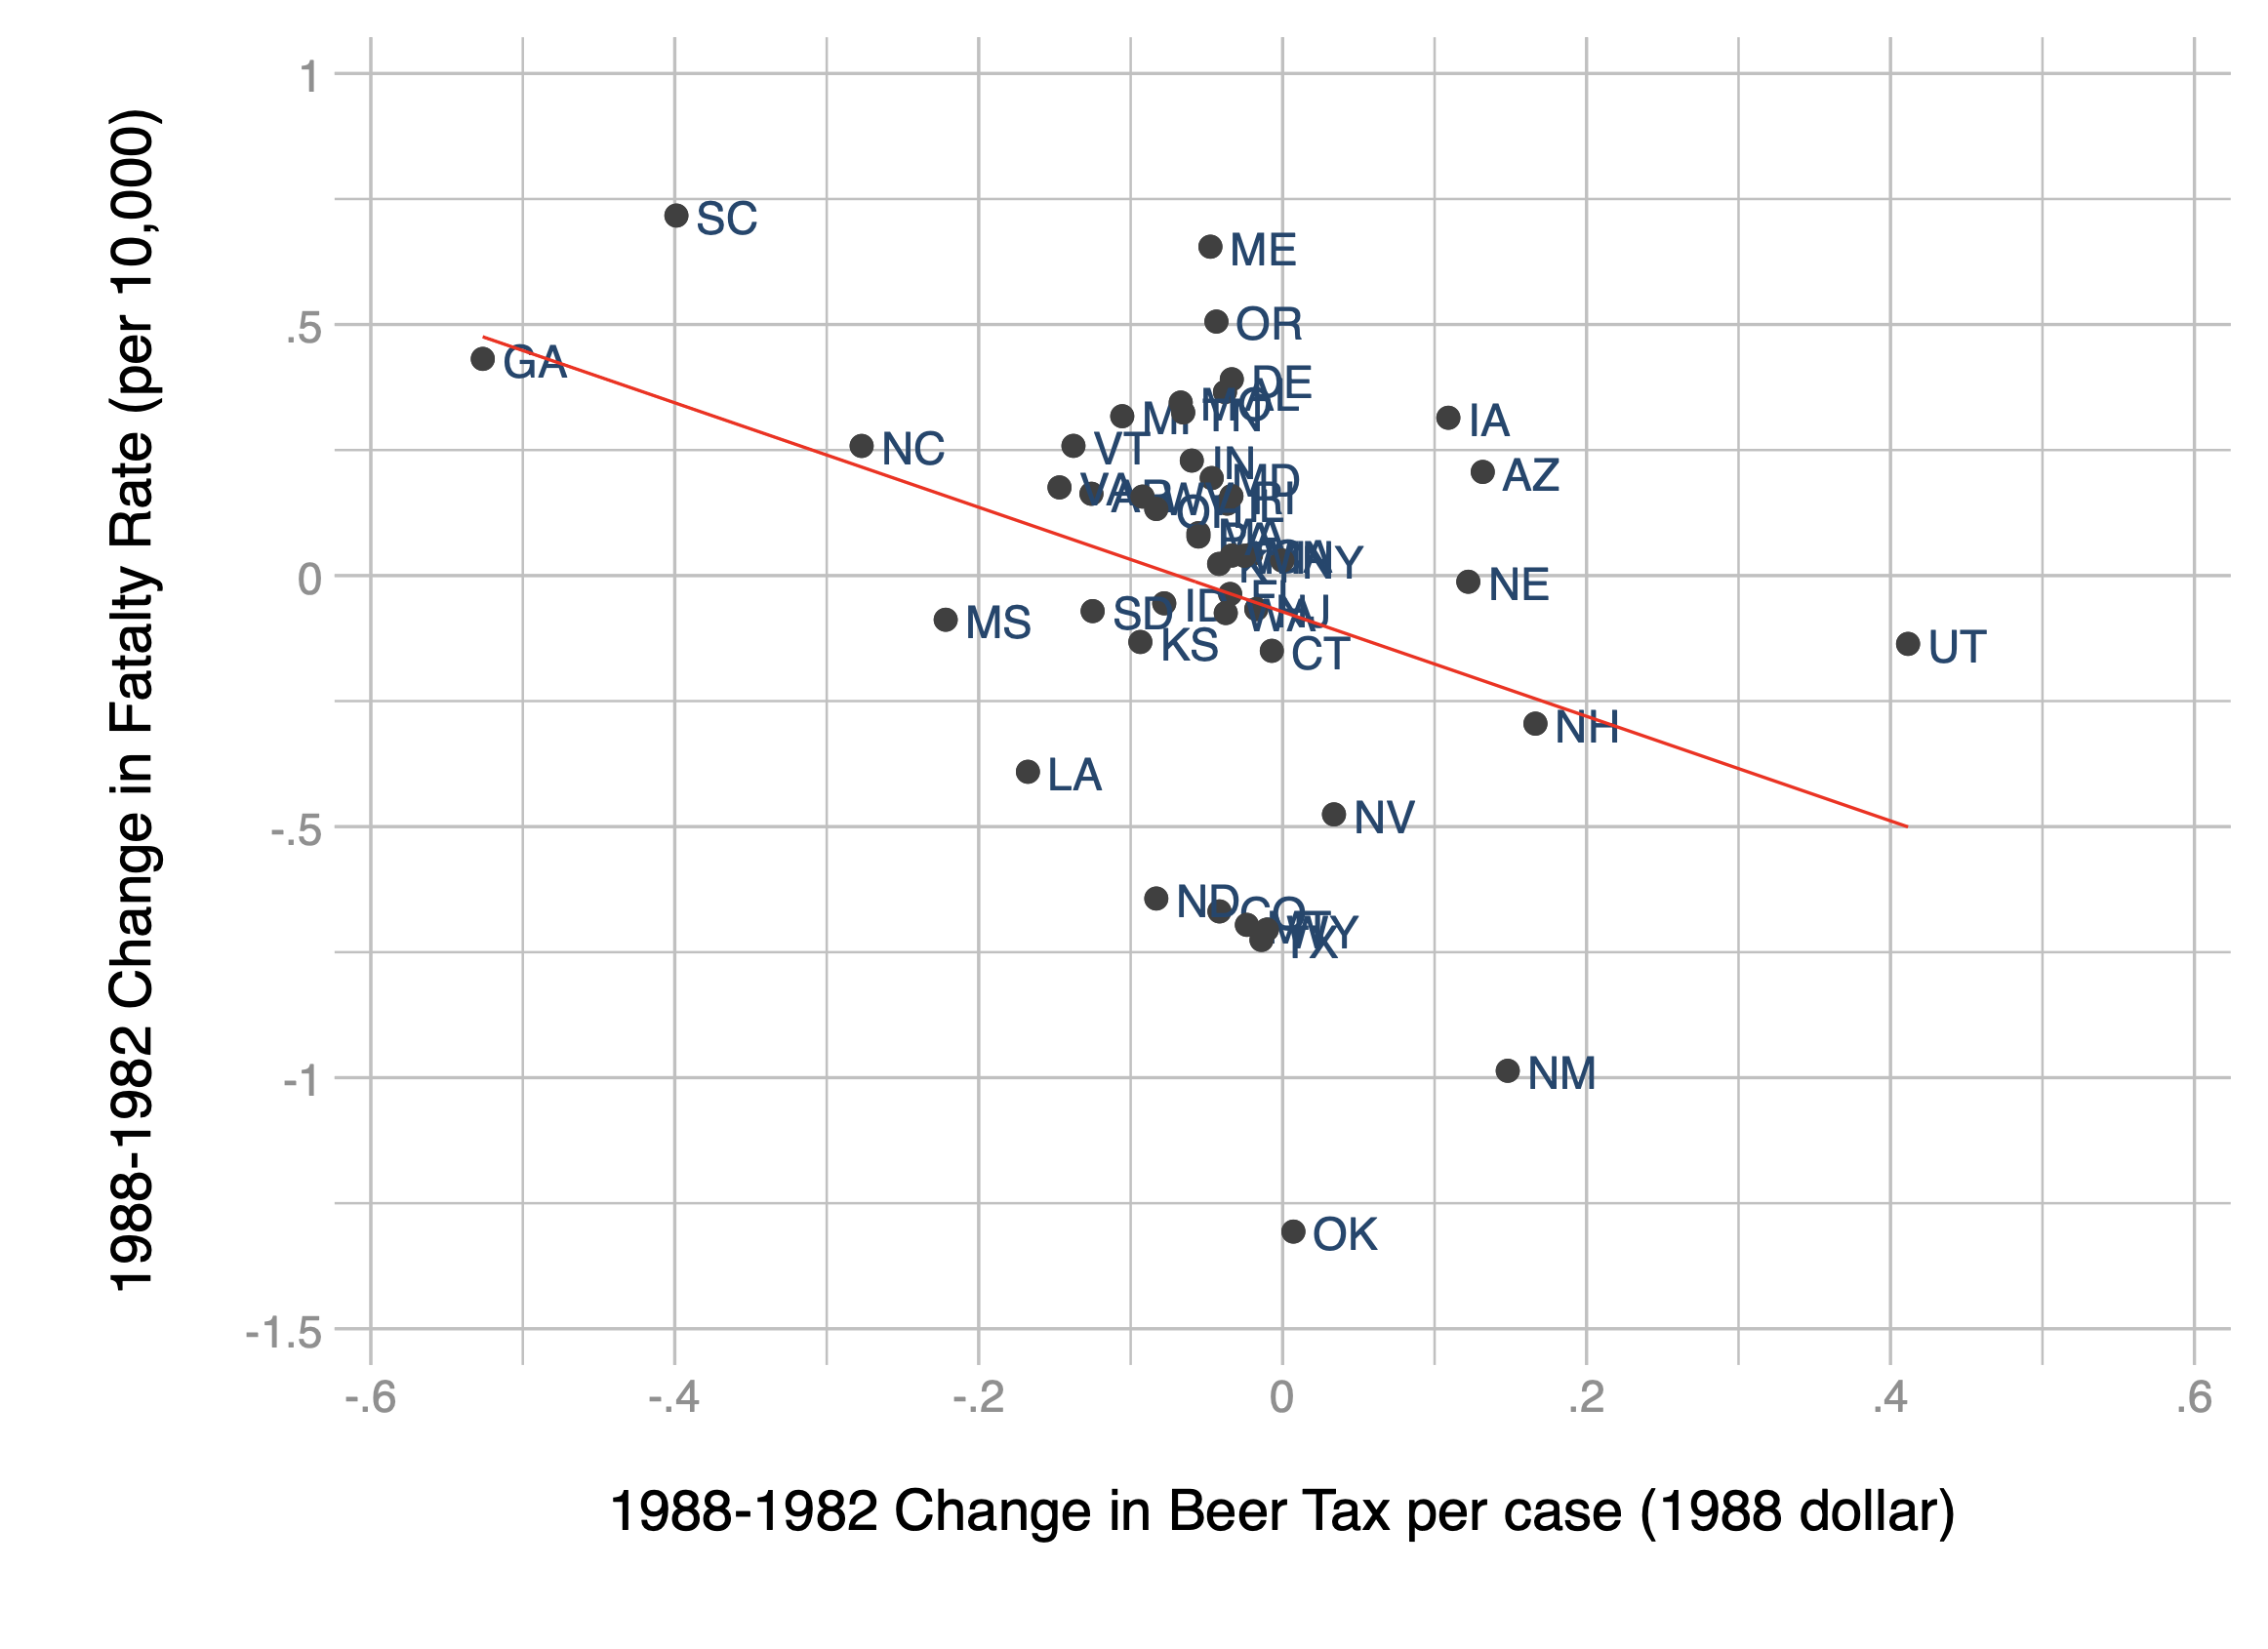
\includegraphics[width=.75\linewidth]{images/beertaxchange.png}
\end{figure}
\end{frame}

\begin{frame}{First Differences when $T>2$}
We can also use differencing with more than two time periods:

\begin{equation*}
    Fatalities_{i,t} = \beta_0 + \delta_1\mathds{1}_{1983} + \delta_2\mathds{1}_{1984}  + \cdots +  \delta_6\mathds{1}_{1988} +\beta_1 BeerTax_{i,t} + \beta_2 Z_i + u_{i,t}
\end{equation*}\\[1em]

That is,
\begin{eqnarray*}
    &Fatalities_{i,1982} = \beta_0 +\beta_1 BeerTax_{i,1982} + \beta_2 Z_i + u_{i,1982}\\
    &Fatalities_{i,1983} = \beta_0 + \delta_1\mathds{1}_{1983} +\beta_1 BeerTax_{i,1983} + \beta_2 Z_i + u_{i,1983}\\
    &Fatalities_{i,1984} = \beta_0 + \delta_2\mathds{1}_{1984} +\beta_1 BeerTax_{i,1984} + \beta_2 Z_i + u_{i,1984}\\
    & \cdots\\
    &Fatalities_{i,1988} = \beta_0 + \delta_6\mathds{1}_{1988} +\beta_1 BeerTax_{i,1988} + \beta_2 Z_i + u_{i,1988}
\end{eqnarray*}\\[1em]
We do so by taking differences between adjacent time periods:
\begin{equation*}
    \Delta Fatalities_{i,t}= \delta_1 + \Delta\delta_2\mathds{1}_{1984}+\cdots+ \Delta\delta_6\mathds{1}_{1988}+ \beta_1  \Delta BeerTax_{i,t} + \Delta u_{i,t}
\end{equation*}
\end{frame}

\begin{frame}{Limits of First-Differences}
\begin{itemize}
    \item The main limitation of using FD compared to other methods is probably that we lose the initial period (there are $N(T-1)$ observations)\\[1em]
    \item Because FD builds on ensuing observations, missing data can be very problematic (imagine if we only observe some $i$ once every other year)\\[1em]
    \item Typically, the variation in the differenced independent variable is much smaller than the variation in the original independent variable. Thus, imprecise estimates could happen from the FD estimator.\\[1em]
    \item Serial correlation (more on that later)\\[1em]
    \item First differencing can enlarge classical errors-in-variable (i.e., measurement error) bias\\[1em]
\end{itemize}
\end{frame}


\section{Fixed Effects Models}

\begin{frame}
  \vfill
  \centering
    {\huge \color{blue} \textit{Fixed Effects Models}}
  \vfill
\end{frame}


{ % all template changes are local to this group.
    \setbeamertemplate{navigation symbols}{}
    \begin{frame}<article:0>[plain]
        \begin{tikzpicture}[remember picture,overlay]
            \node[at=(current page.center)] {
                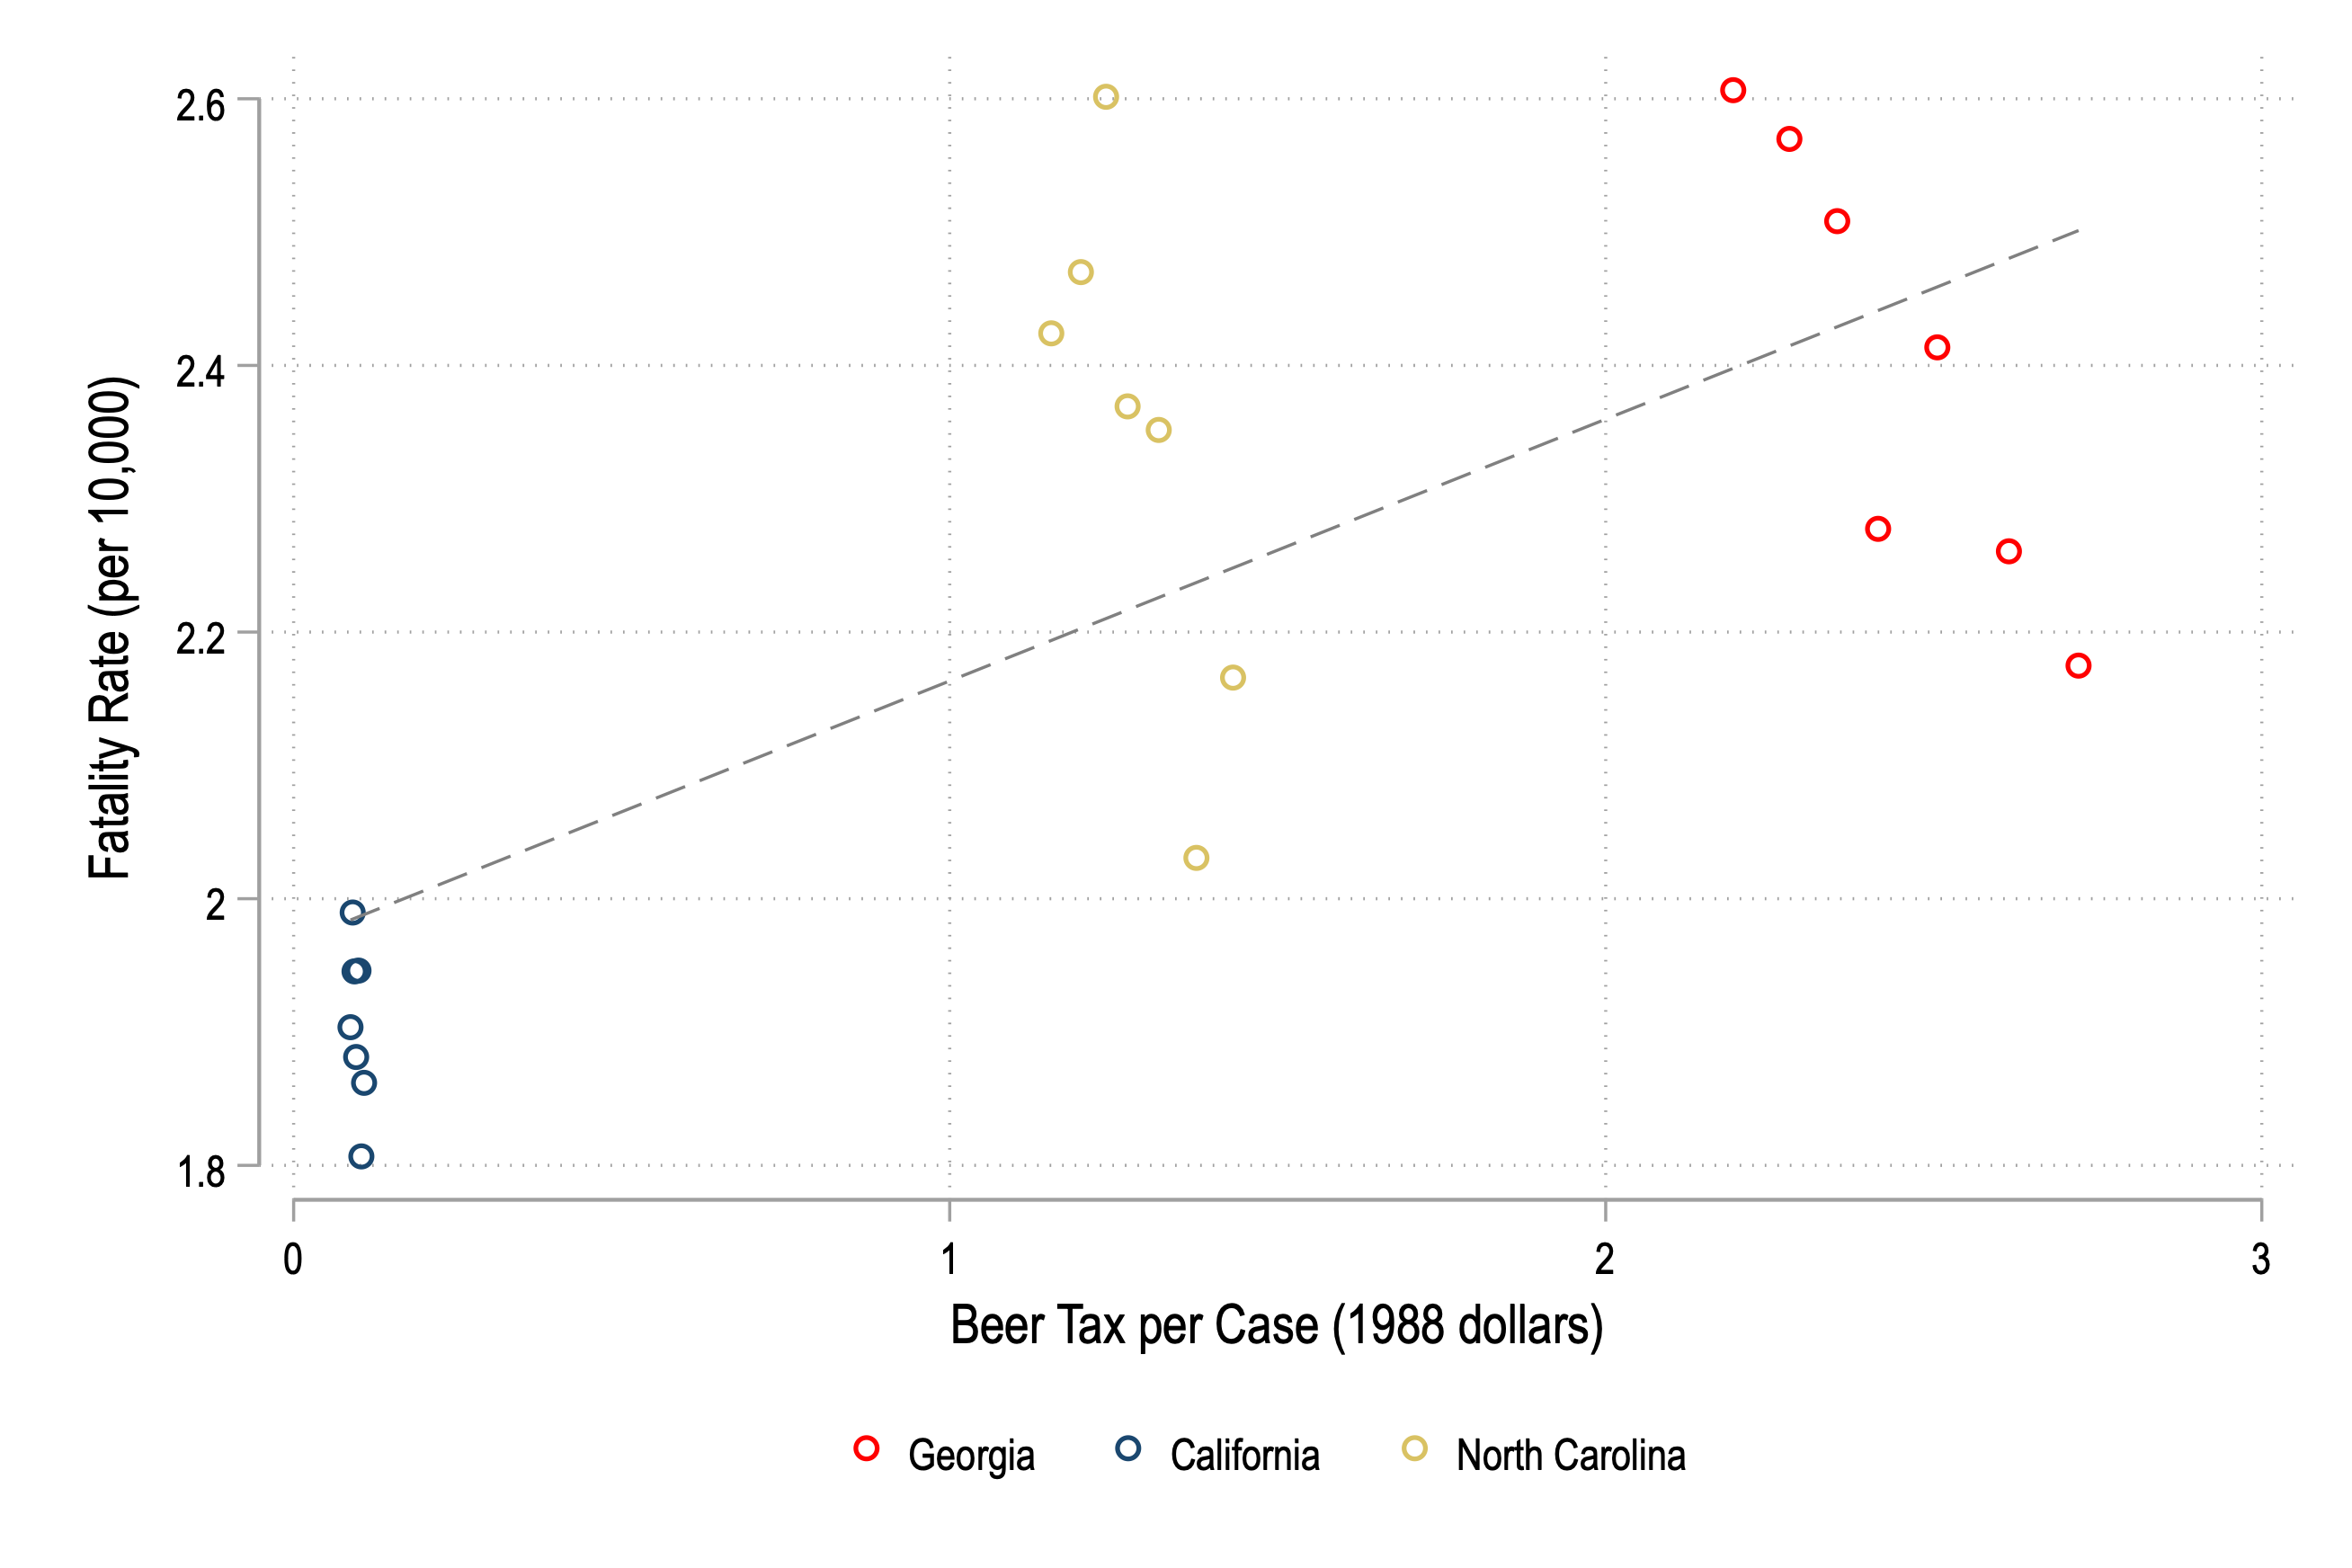
\includegraphics[keepaspectratio,
                                 width=.9\paperwidth,
                                 height=.9\paperheight]{images/fe0.png}
            };
        \end{tikzpicture}
     \end{frame}
}


{ % all template changes are local to this group.
    \setbeamertemplate{navigation symbols}{}
    \begin{frame}<article:0>[plain]
        \begin{tikzpicture}[remember picture,overlay]
            \node[at=(current page.center)] {
                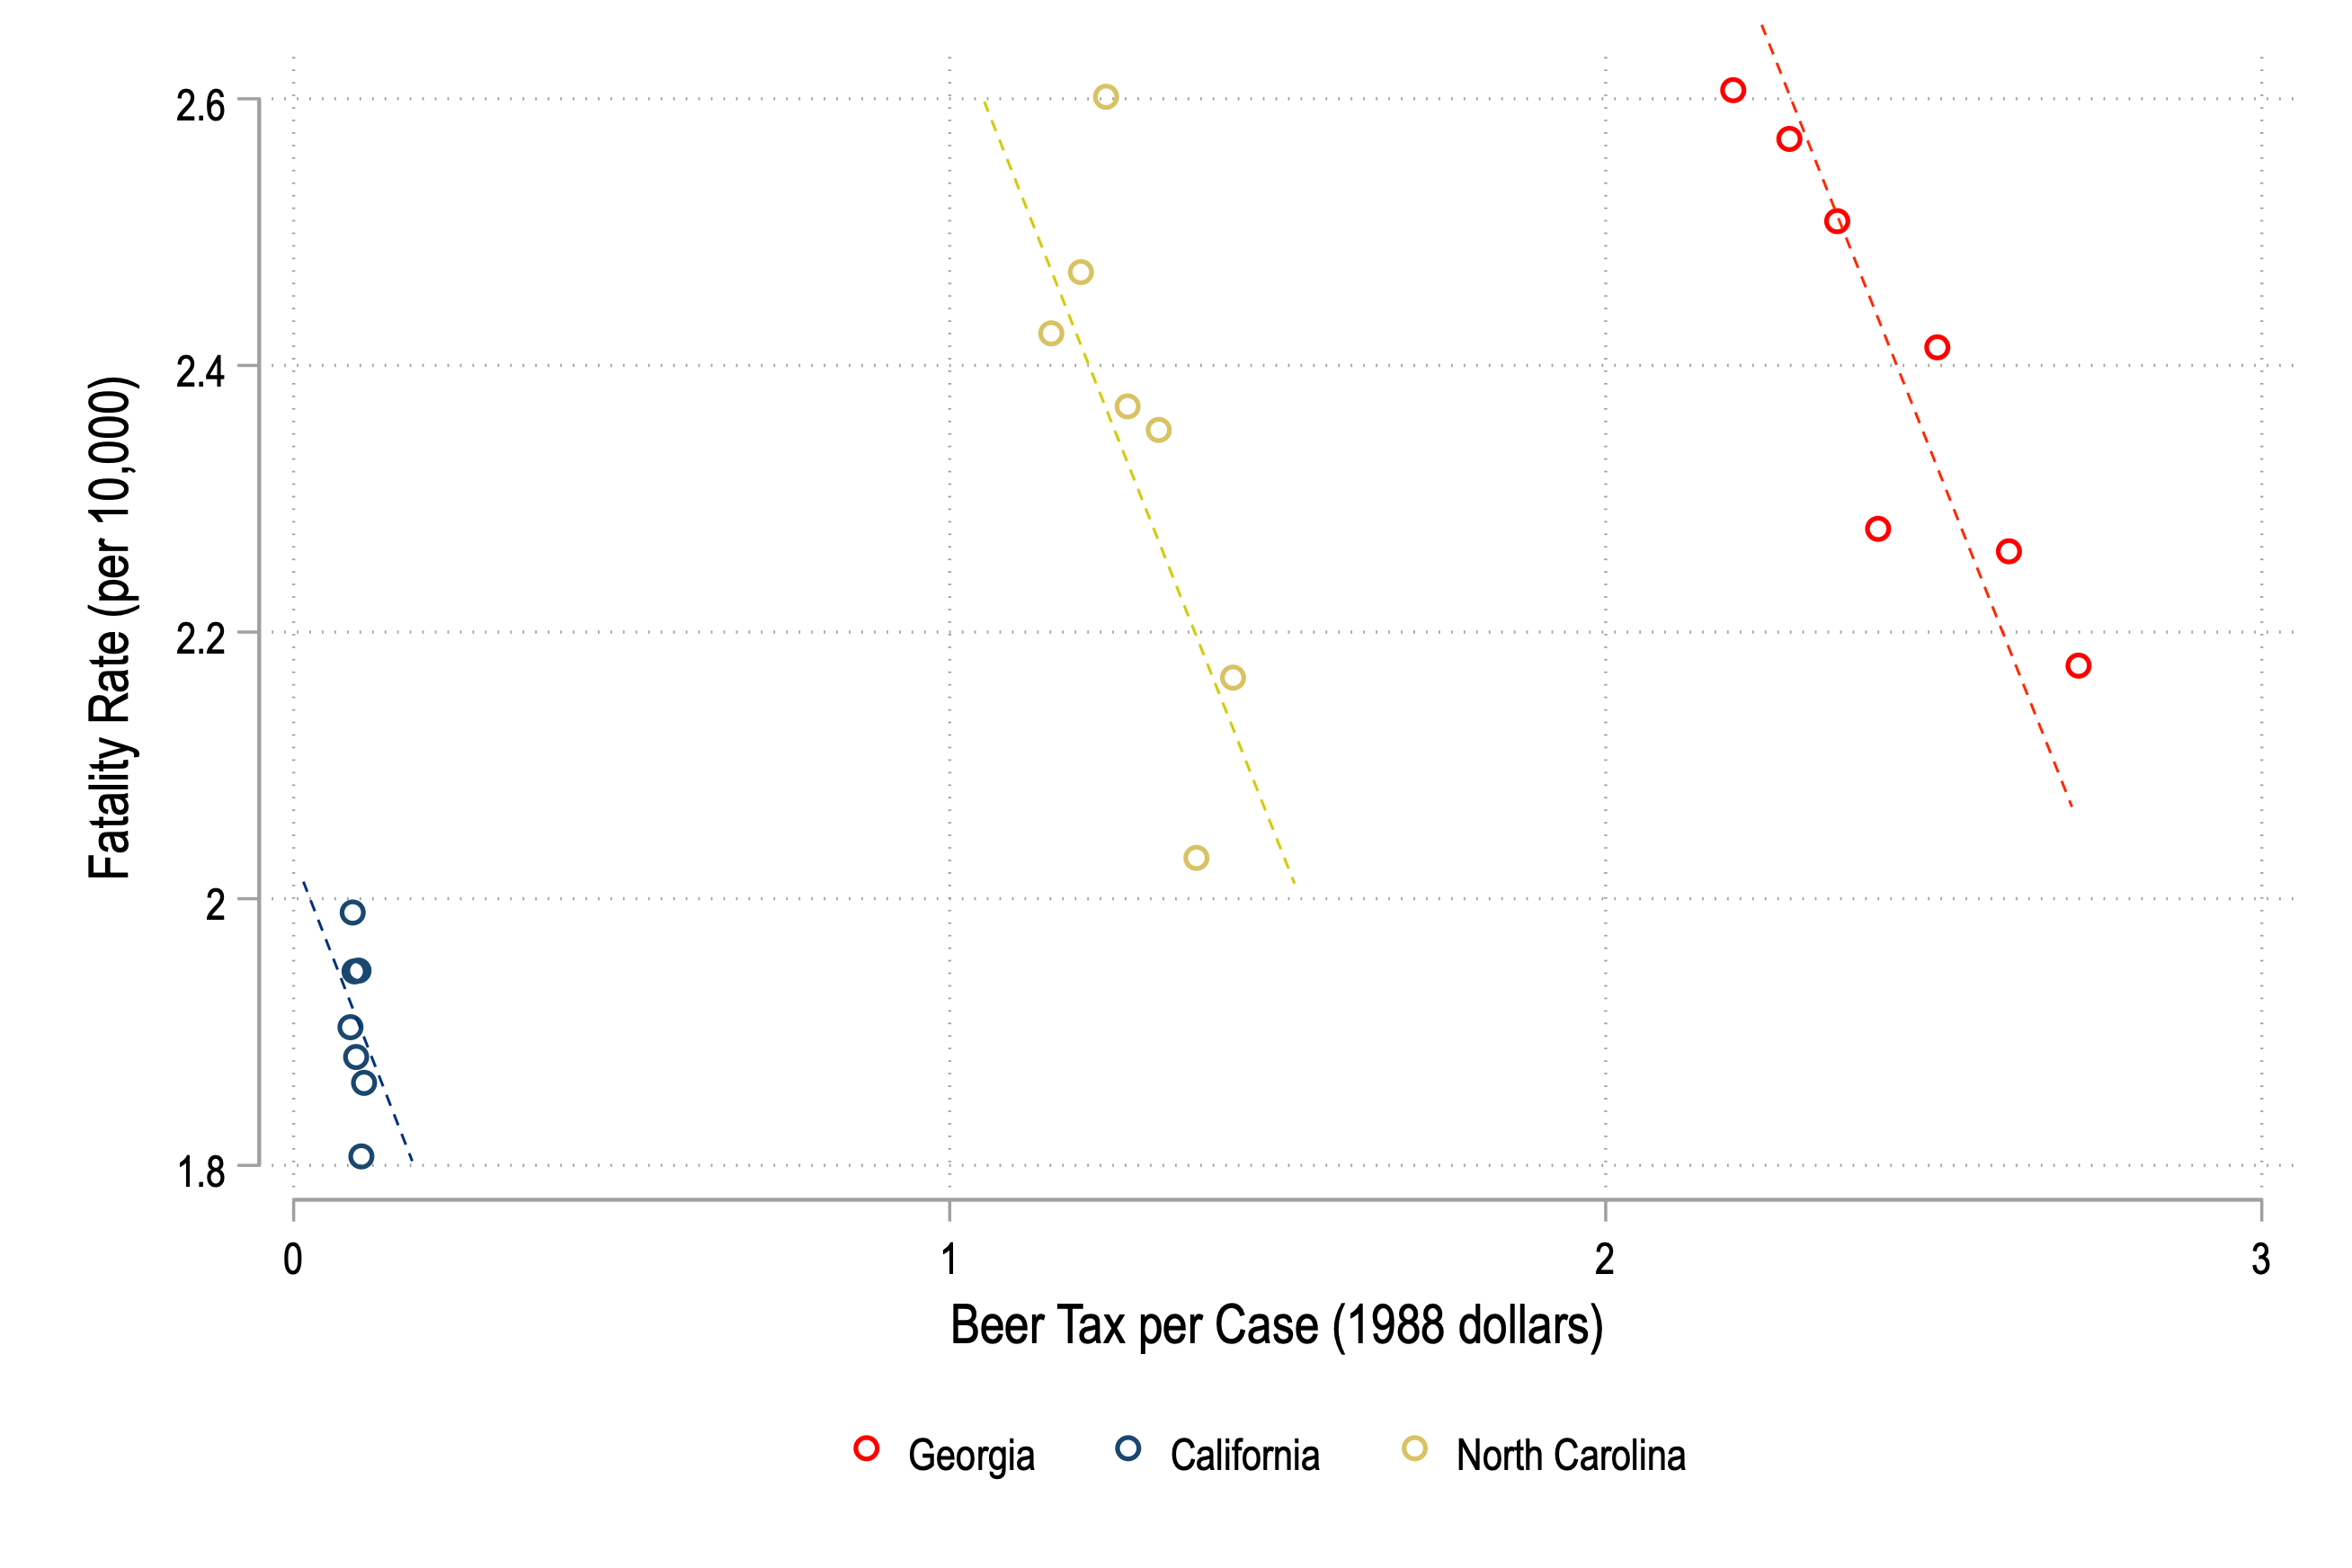
\includegraphics[keepaspectratio,
                                 width=.9\paperwidth,
                                 height=.9\paperheight]{images/fe1bis.png}
            };
        \end{tikzpicture}
     \end{frame}
}



\begin{frame}{Fixed Effects Regressions}
The general FE model reads
\begin{equation*}
    Fatalities_{i,t} = \beta_0 + \beta_1 BeerTax_{i,t} + \beta_2 Z_i + u_{i,t}
\end{equation*}\\[1em]
For example, in the case of California,
\begin{eqnarray*}
    &Fatalities_{CA,t} &= \beta_0 + \beta_1 BeerTax_{CA,t} + \beta_2 Z_{CA} + u_{CA,t}\\
    & &= (\beta_0 + \beta_2 Z_{CA}) + \beta_1 BeerTax_{CA,t}  + u_{CA,t}\\
    & &= \alpha_{CA} + \beta_1 BeerTax_{CA,t}  + u_{CA,t}
\end{eqnarray*}\\[1em]
Where $\alpha_{CA}$ is the intercept for California, and $\beta_1$ is the slope.\\[1em]
The intercept is unique to CA, but the slope is the same in all the states: parallel lines.
\end{frame}

\begin{frame}{Fixed Effects Regressions}
 \begin{columns}
\begin{column}{0.35\textwidth}
Two equivalent ways of writing the same specification:\\[1em]
    \begin{eqnarray*}
        Y_{i,t} = \beta_0 + \beta_1 X_{i,t} + \gamma_1 D_{i}\mid_{i=1}\\
        + \gamma_2 D_{i}\mid_{i=2}+ \dots + \gamma_n D_{i}\mid_{i=n} + u_{i,t}
    \end{eqnarray*}
where $D_{i}\mid_{i=n} = 1$ if $i=n$ (i.e., state \#$n$).\\[1em] And,
    \begin{equation*}
        Y_{i,t} = \alpha_i + \beta_1 X_{i,t}  + u_{i,t}
    \end{equation*}
\end{column}
\begin{column}{0.7\textwidth}
\begin{figure}
  \centering
         \vspace{-1mm}
        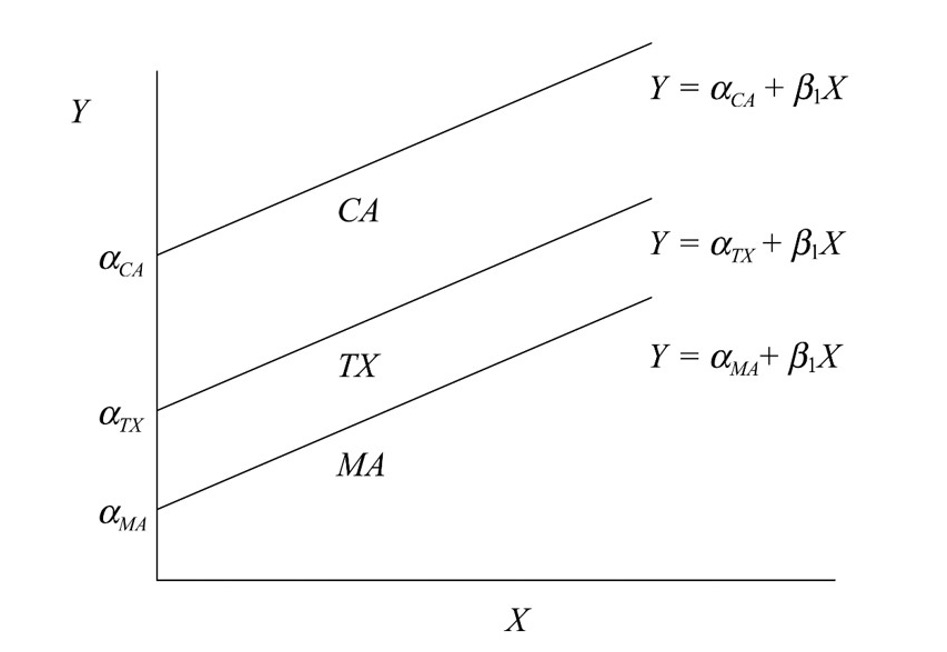
\includegraphics[scale=.3]{images/fixedeffects0.jpg}
\end{figure}
\end{column}
\end{columns}
\end{frame}


\begin{frame}{Fixed Effects Regressions}
Including $n$ extra (fixed effect) dummies can be computationally intensive when $n$ is large. What regression softwares typically do is to (time-)\textit{demean} (\textbf{within transformation}) the specification:
    \begin{equation*}
        \bar{Y}_i = \alpha_i + \frac{1}{T}\sum_{t=1}^T \beta_1 X_{i,t}  + \frac{1}{T}\sum_{t=1}^T  u_{i,t}
    \end{equation*}
Which yields to
    \begin{equation*}
        Y_{i,t} - \bar{Y}_i =  \beta_1 (X_{i,t}-\frac{1}{T}\sum_{t=1}^T X_{i,t})  + (u_{i,t}-\frac{1}{T}\sum_{t=1}^T  u_{i,t})
    \end{equation*}
which can be estimated by simple OLS, that is
    \begin{equation*}
        \tilde{Y}_{i,t}= \beta_1 \tilde{X}_{i,t} + \tilde{u}_{i,t}
    \end{equation*}
and $\beta_1$ isolates the impact of changes in $X$ within a unit, ignoring the constant, unit-specific factors influencing both $X$ and $Y$.
\end{frame}

\begin{frame}{Fixed Effects Regressions}
\begin{figure}
  \centering
         \vspace{-1mm}
         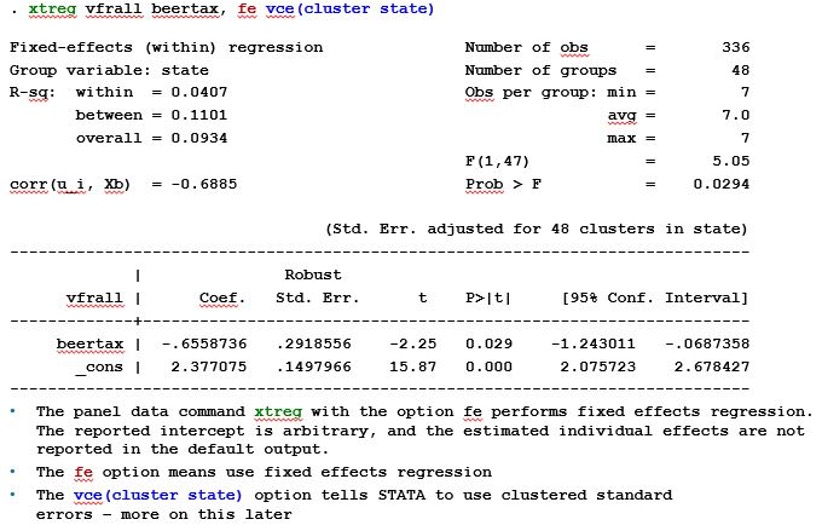
\includegraphics[width=.75\linewidth]{images/fixedeffects1.jpg}
\end{figure}
\end{frame}


\begin{frame}{Fixed Effects Regressions}
By analogy, we can also include time FEs (i.e., they are the same across unit but vary in time). What omitted variable could be captured by time FEs in the traffic fatalities vs. beer taxes case?\\[1em]

The population line for, say, 1985 reads
\begin{eqnarray*}
    &Fatalities_{i,1985} &= \beta_0 + \beta_1 BeerTax_{i,1985} + \beta_2 Z_{1985} + u_{i,1985}\\
    & &= (\beta_0 + \beta_2 Z_{1985}) + \beta_1 BeerTax_{i,1985}  + u_{i,1985}\\
    & &= \lambda_{1985} + \beta_1 BeerTax_{i,1985}  + u_{i,1985}
\end{eqnarray*}\\[1em]
Where $\lambda_{1985}$ is the intercept for 1985, and $\beta_1$ is the slope.\\[1em]

The dummies notation holds, as in the preceding example with unit FEs.

\end{frame}


\begin{frame}{Fixed Effects Regressions}
Including $T$ extra (fixed effect) dummies can be computationally intensive when $T$ is large. As before, we can transform the panel model specification into a simple OLS one by demeaning:
    \begin{equation*}
        \bar{Y}_t = \lambda_t + \frac{1}{n}\sum_{i=1}^n \beta_1 X_{i,t}  + \frac{1}{n}\sum_{i=1}^n  u_{i,t}
    \end{equation*}
Which yields to
    \begin{equation*}
        Y_{i,t} - \bar{Y}_t =  \beta_1 (X_{i,t}-\frac{1}{n}\sum_{i=1}^n X_{i,t})  + (u_{i,t}-\frac{1}{n}\sum_{i=1}^n  u_{i,t})
    \end{equation*}
which can be estimated by simple OLS, that is
    \begin{equation*}
        \check{Y}_{i,t}= \beta_1 \check{X}_{i,t} + \check{u}_{i,t}
    \end{equation*}
and $\beta_1$ captures the effect of changes in $X$ within a specific time period, accounting for shared temporal factors that affect both $X$ and $Y$ at the same time.
\end{frame}

\begin{frame}{Raw Panel Data}
\begin{figure}
  \centering
         \vspace{-1mm}
         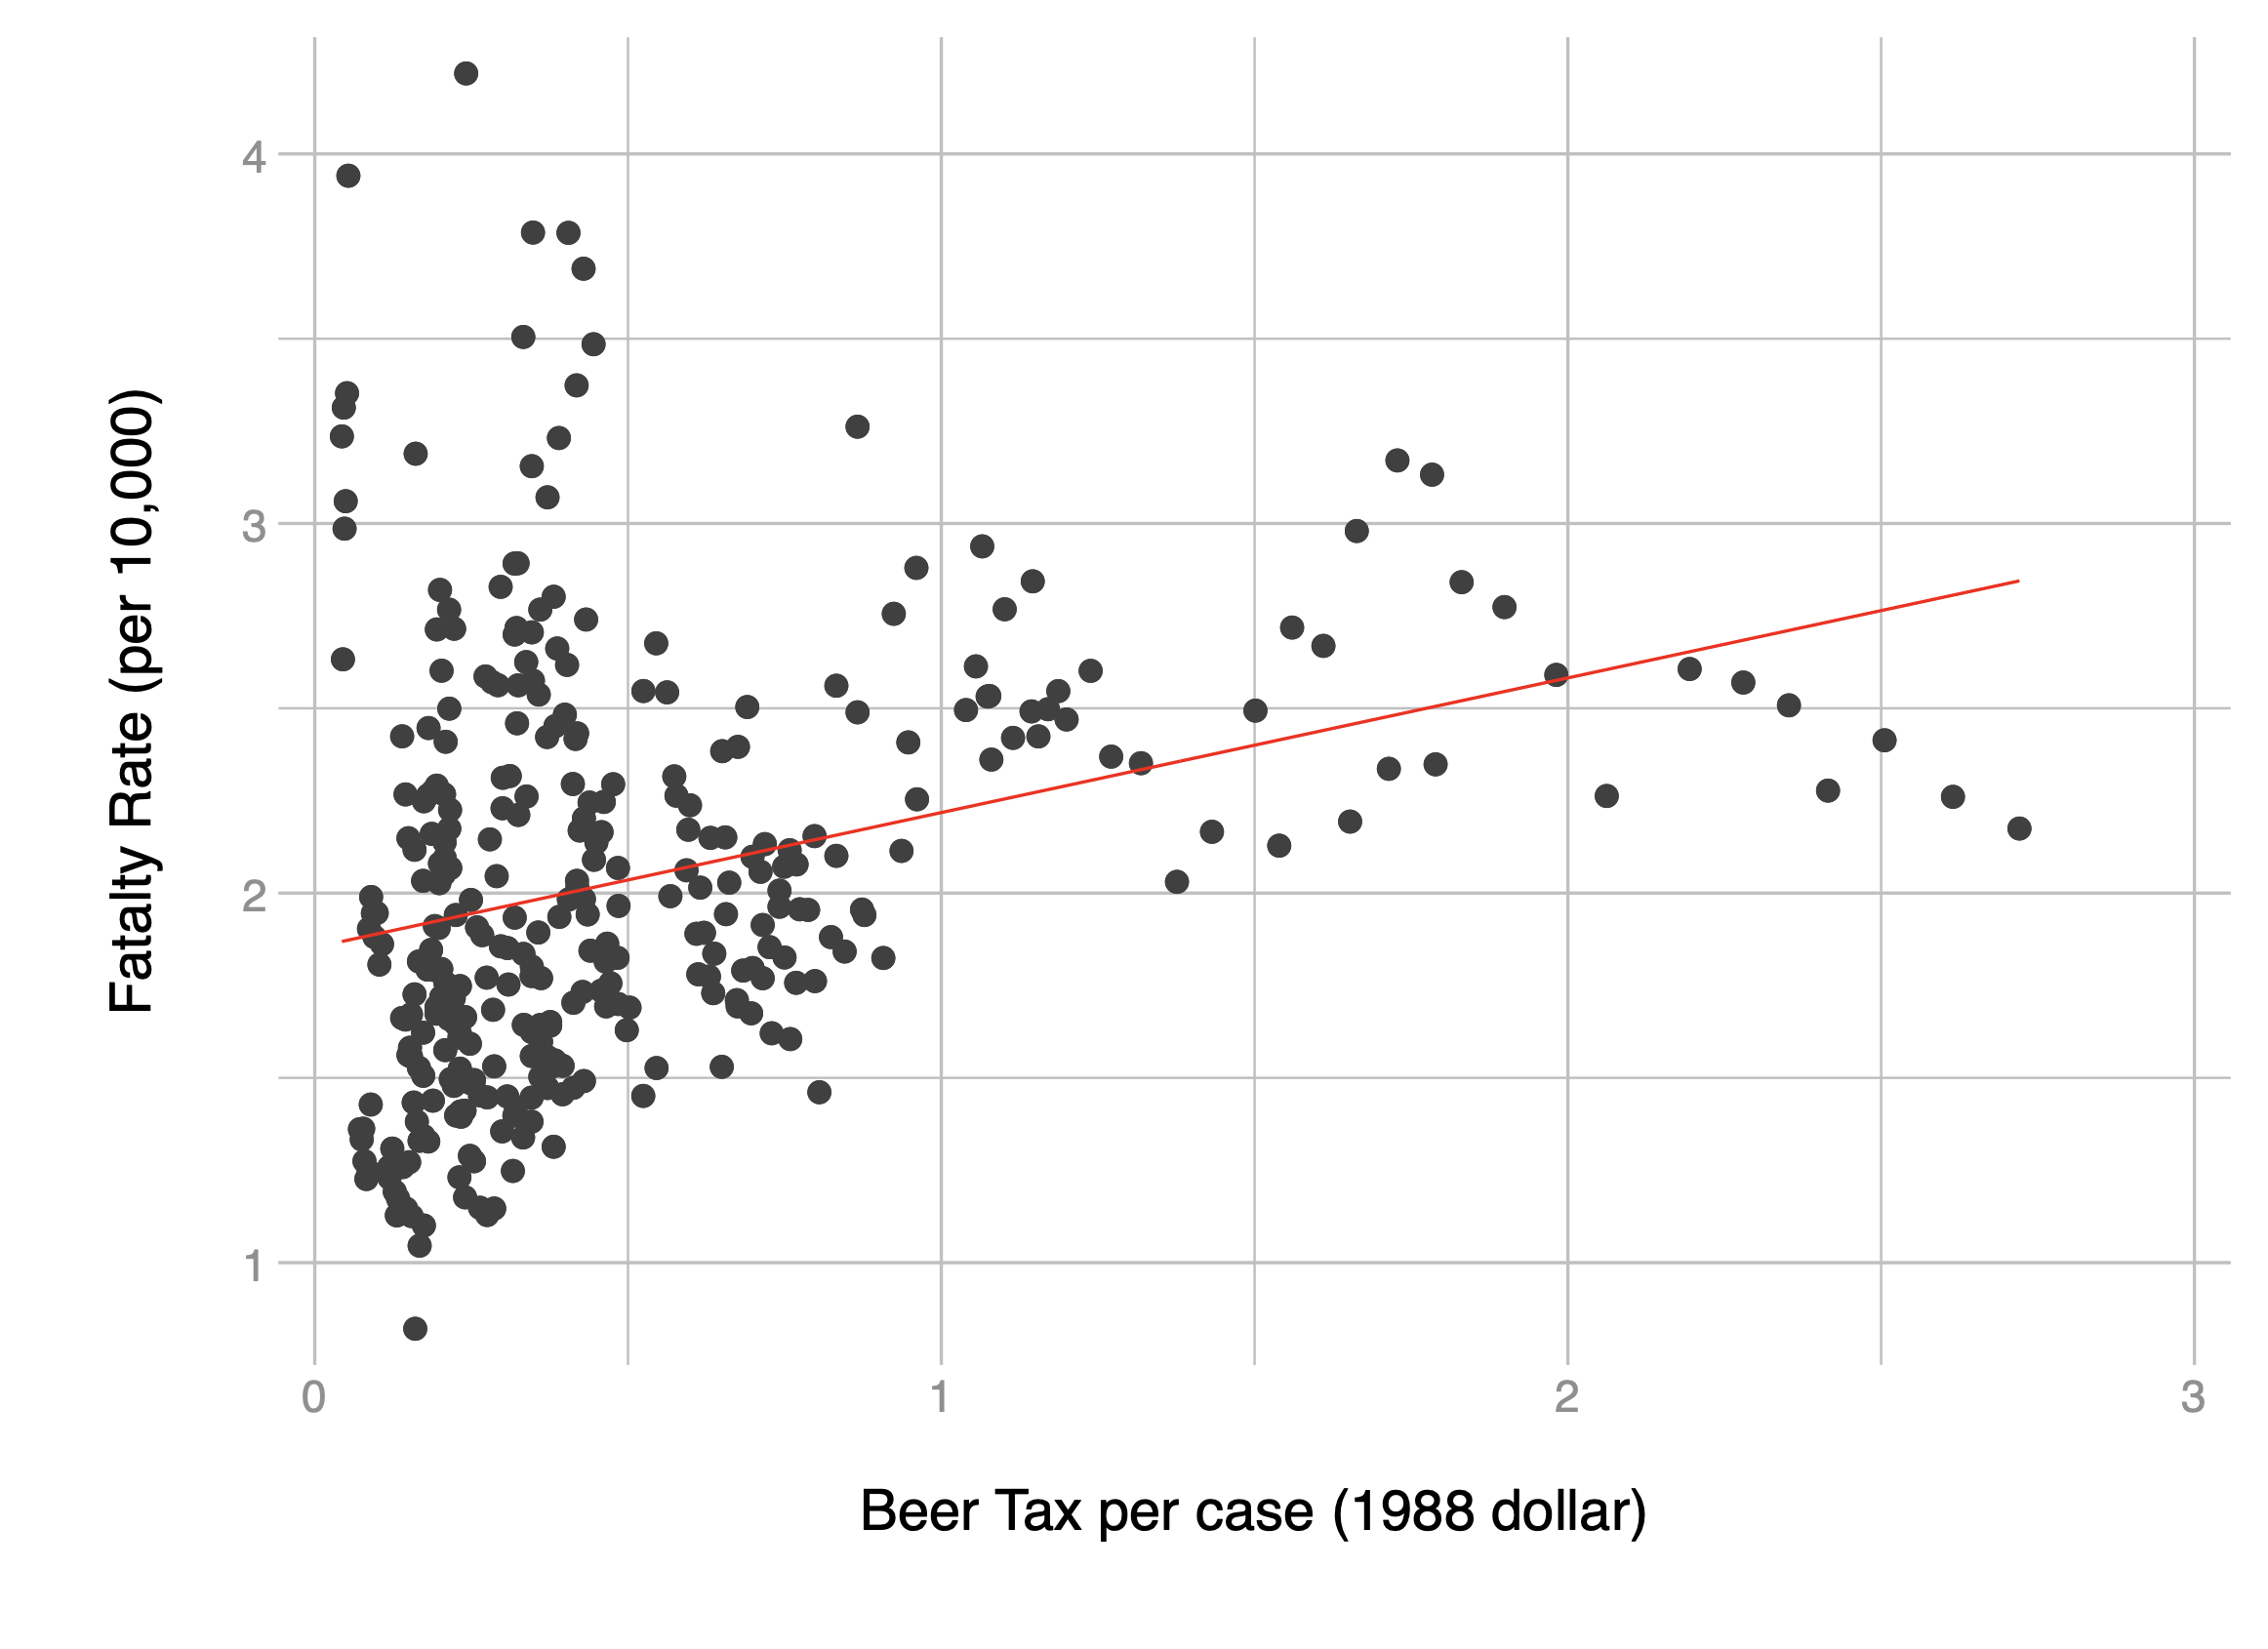
\includegraphics[width=.75\linewidth]{images/beertax_panel0.png}
\end{figure}
\end{frame}

\begin{frame}{Accounting for $\alpha_i$}
\begin{figure}
  \centering
         \vspace{-1mm}
         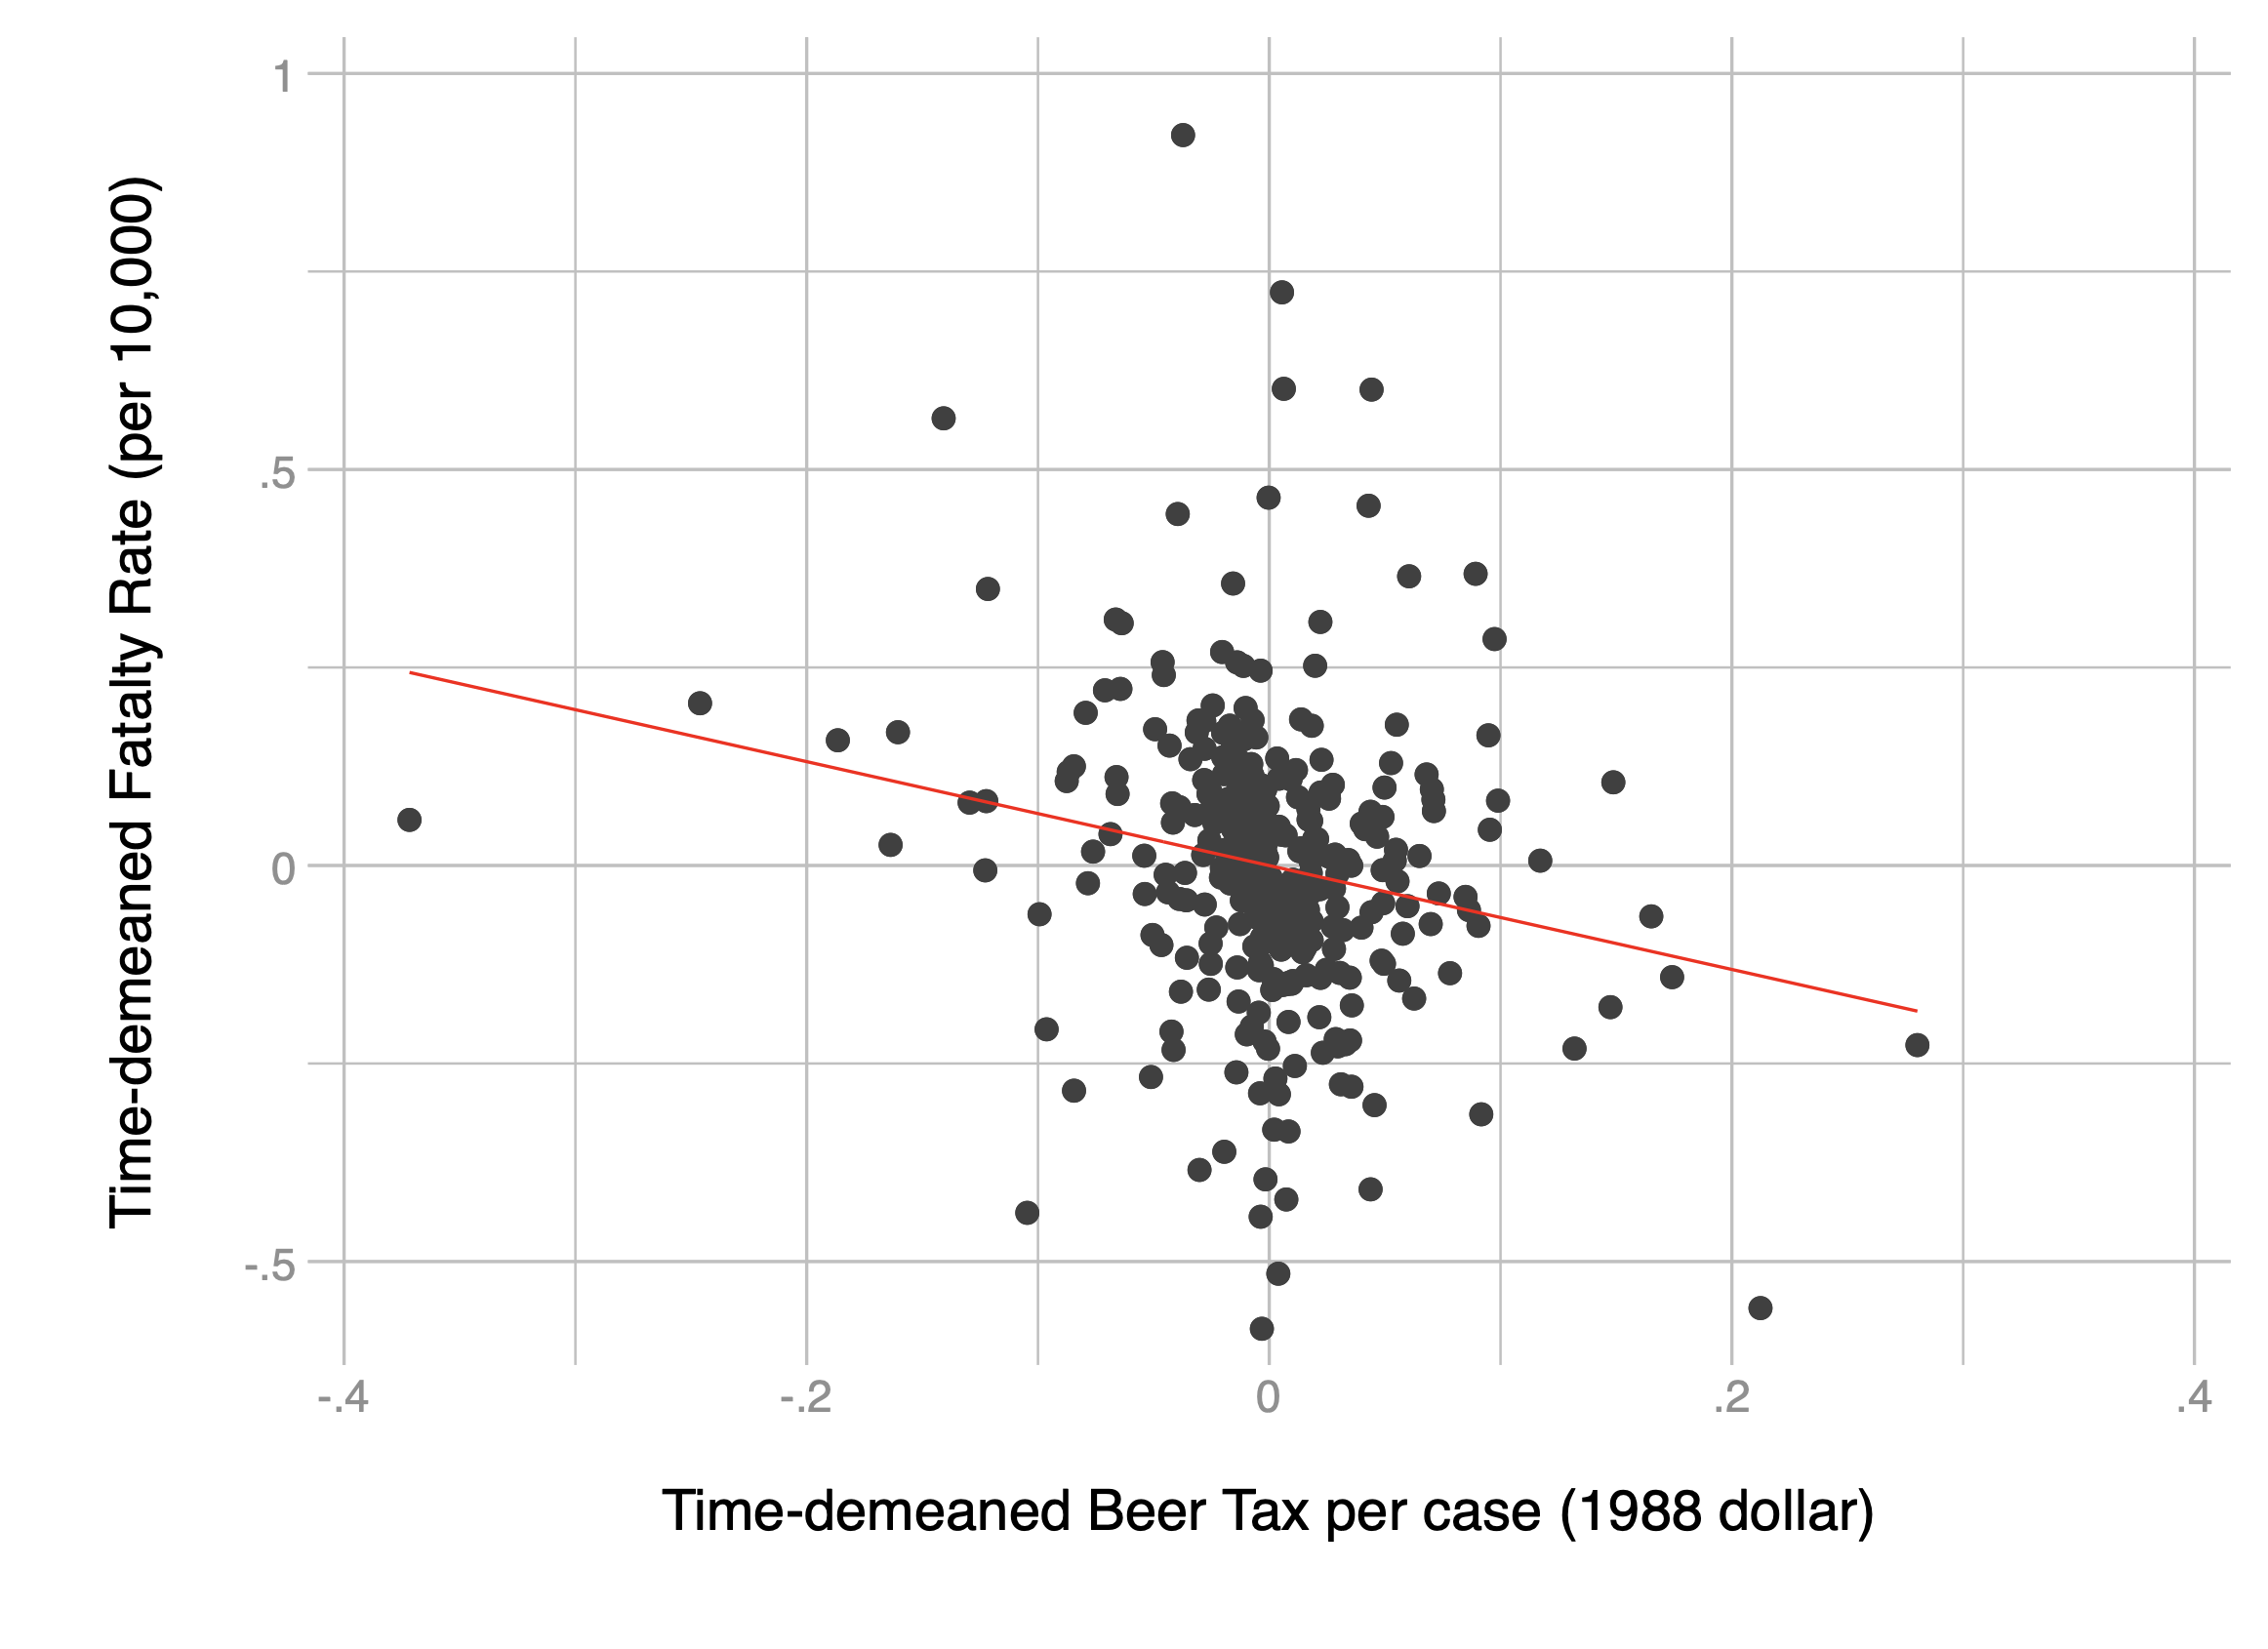
\includegraphics[width=.75\linewidth]{images/beertax_panel1.png}
\end{figure}
\end{frame}

\begin{frame}{Accounting for $\lambda_t$}
\begin{figure}
  \centering
         \vspace{-1mm}
         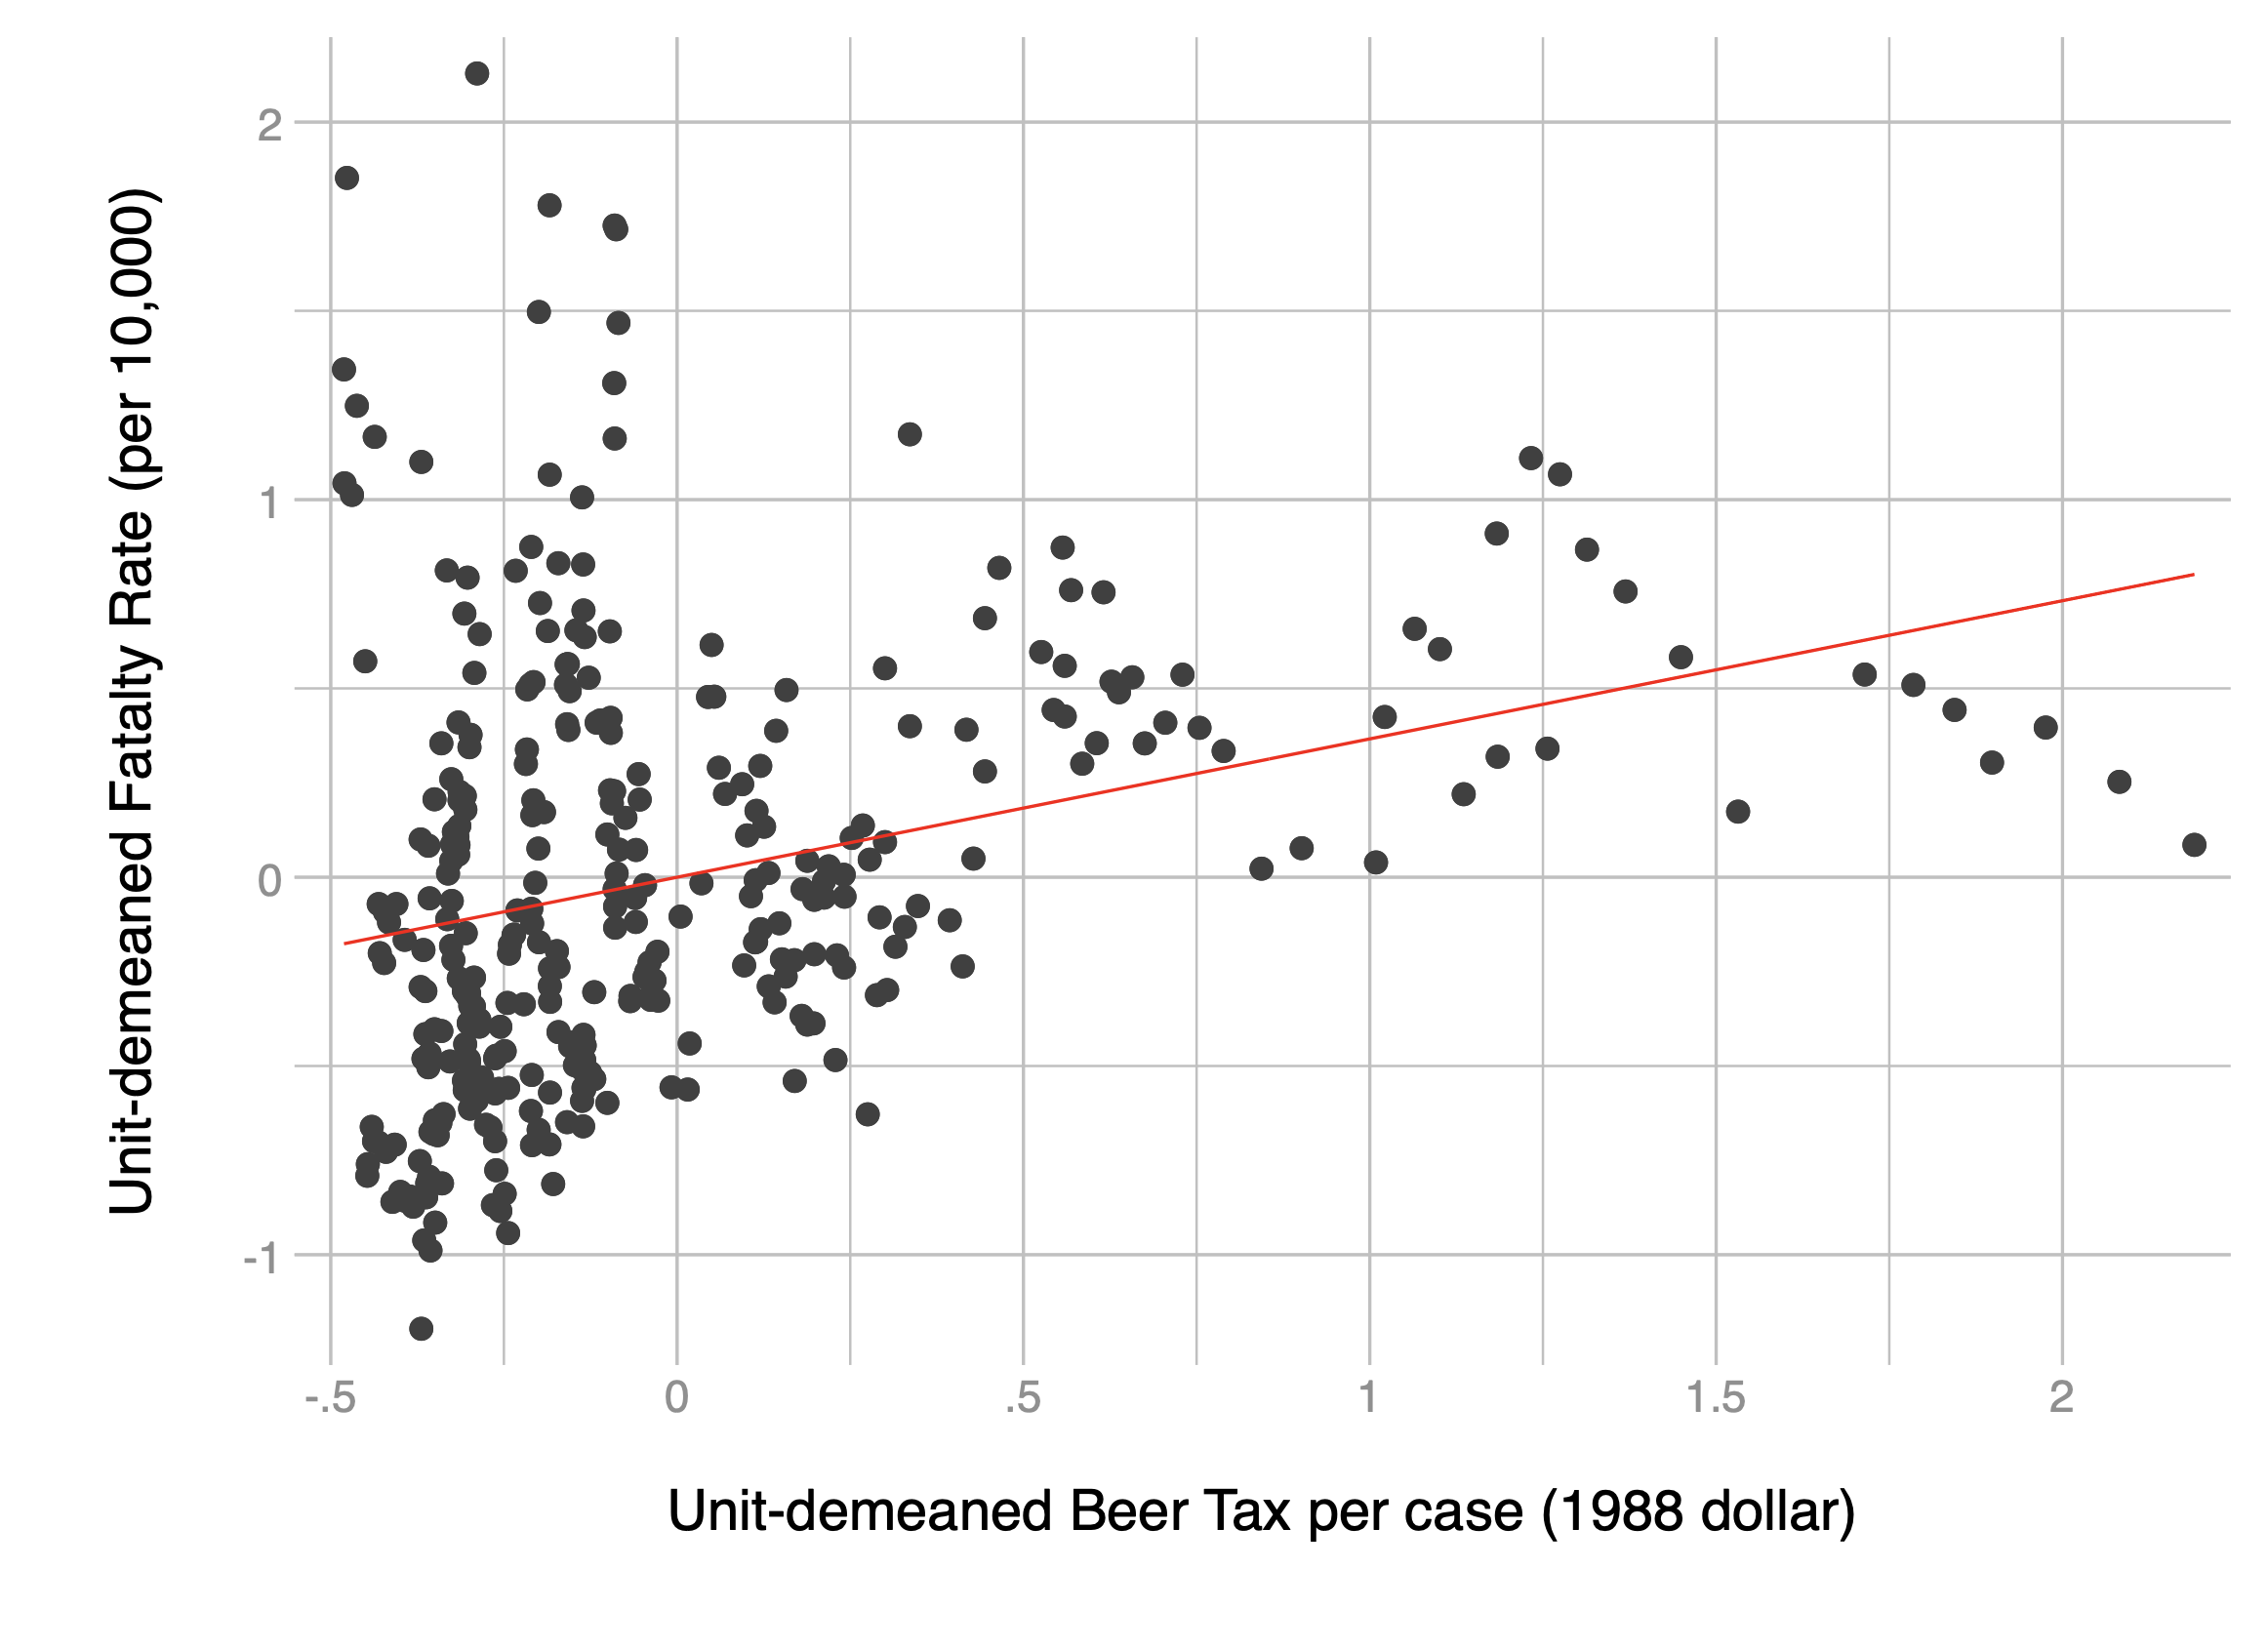
\includegraphics[width=.75\linewidth]{images/beertax_panel2.png}
\end{figure}
\end{frame}

\begin{frame}{Both unit and time fixed effects}
\begin{figure}
  \centering
         \vspace{-1mm}
         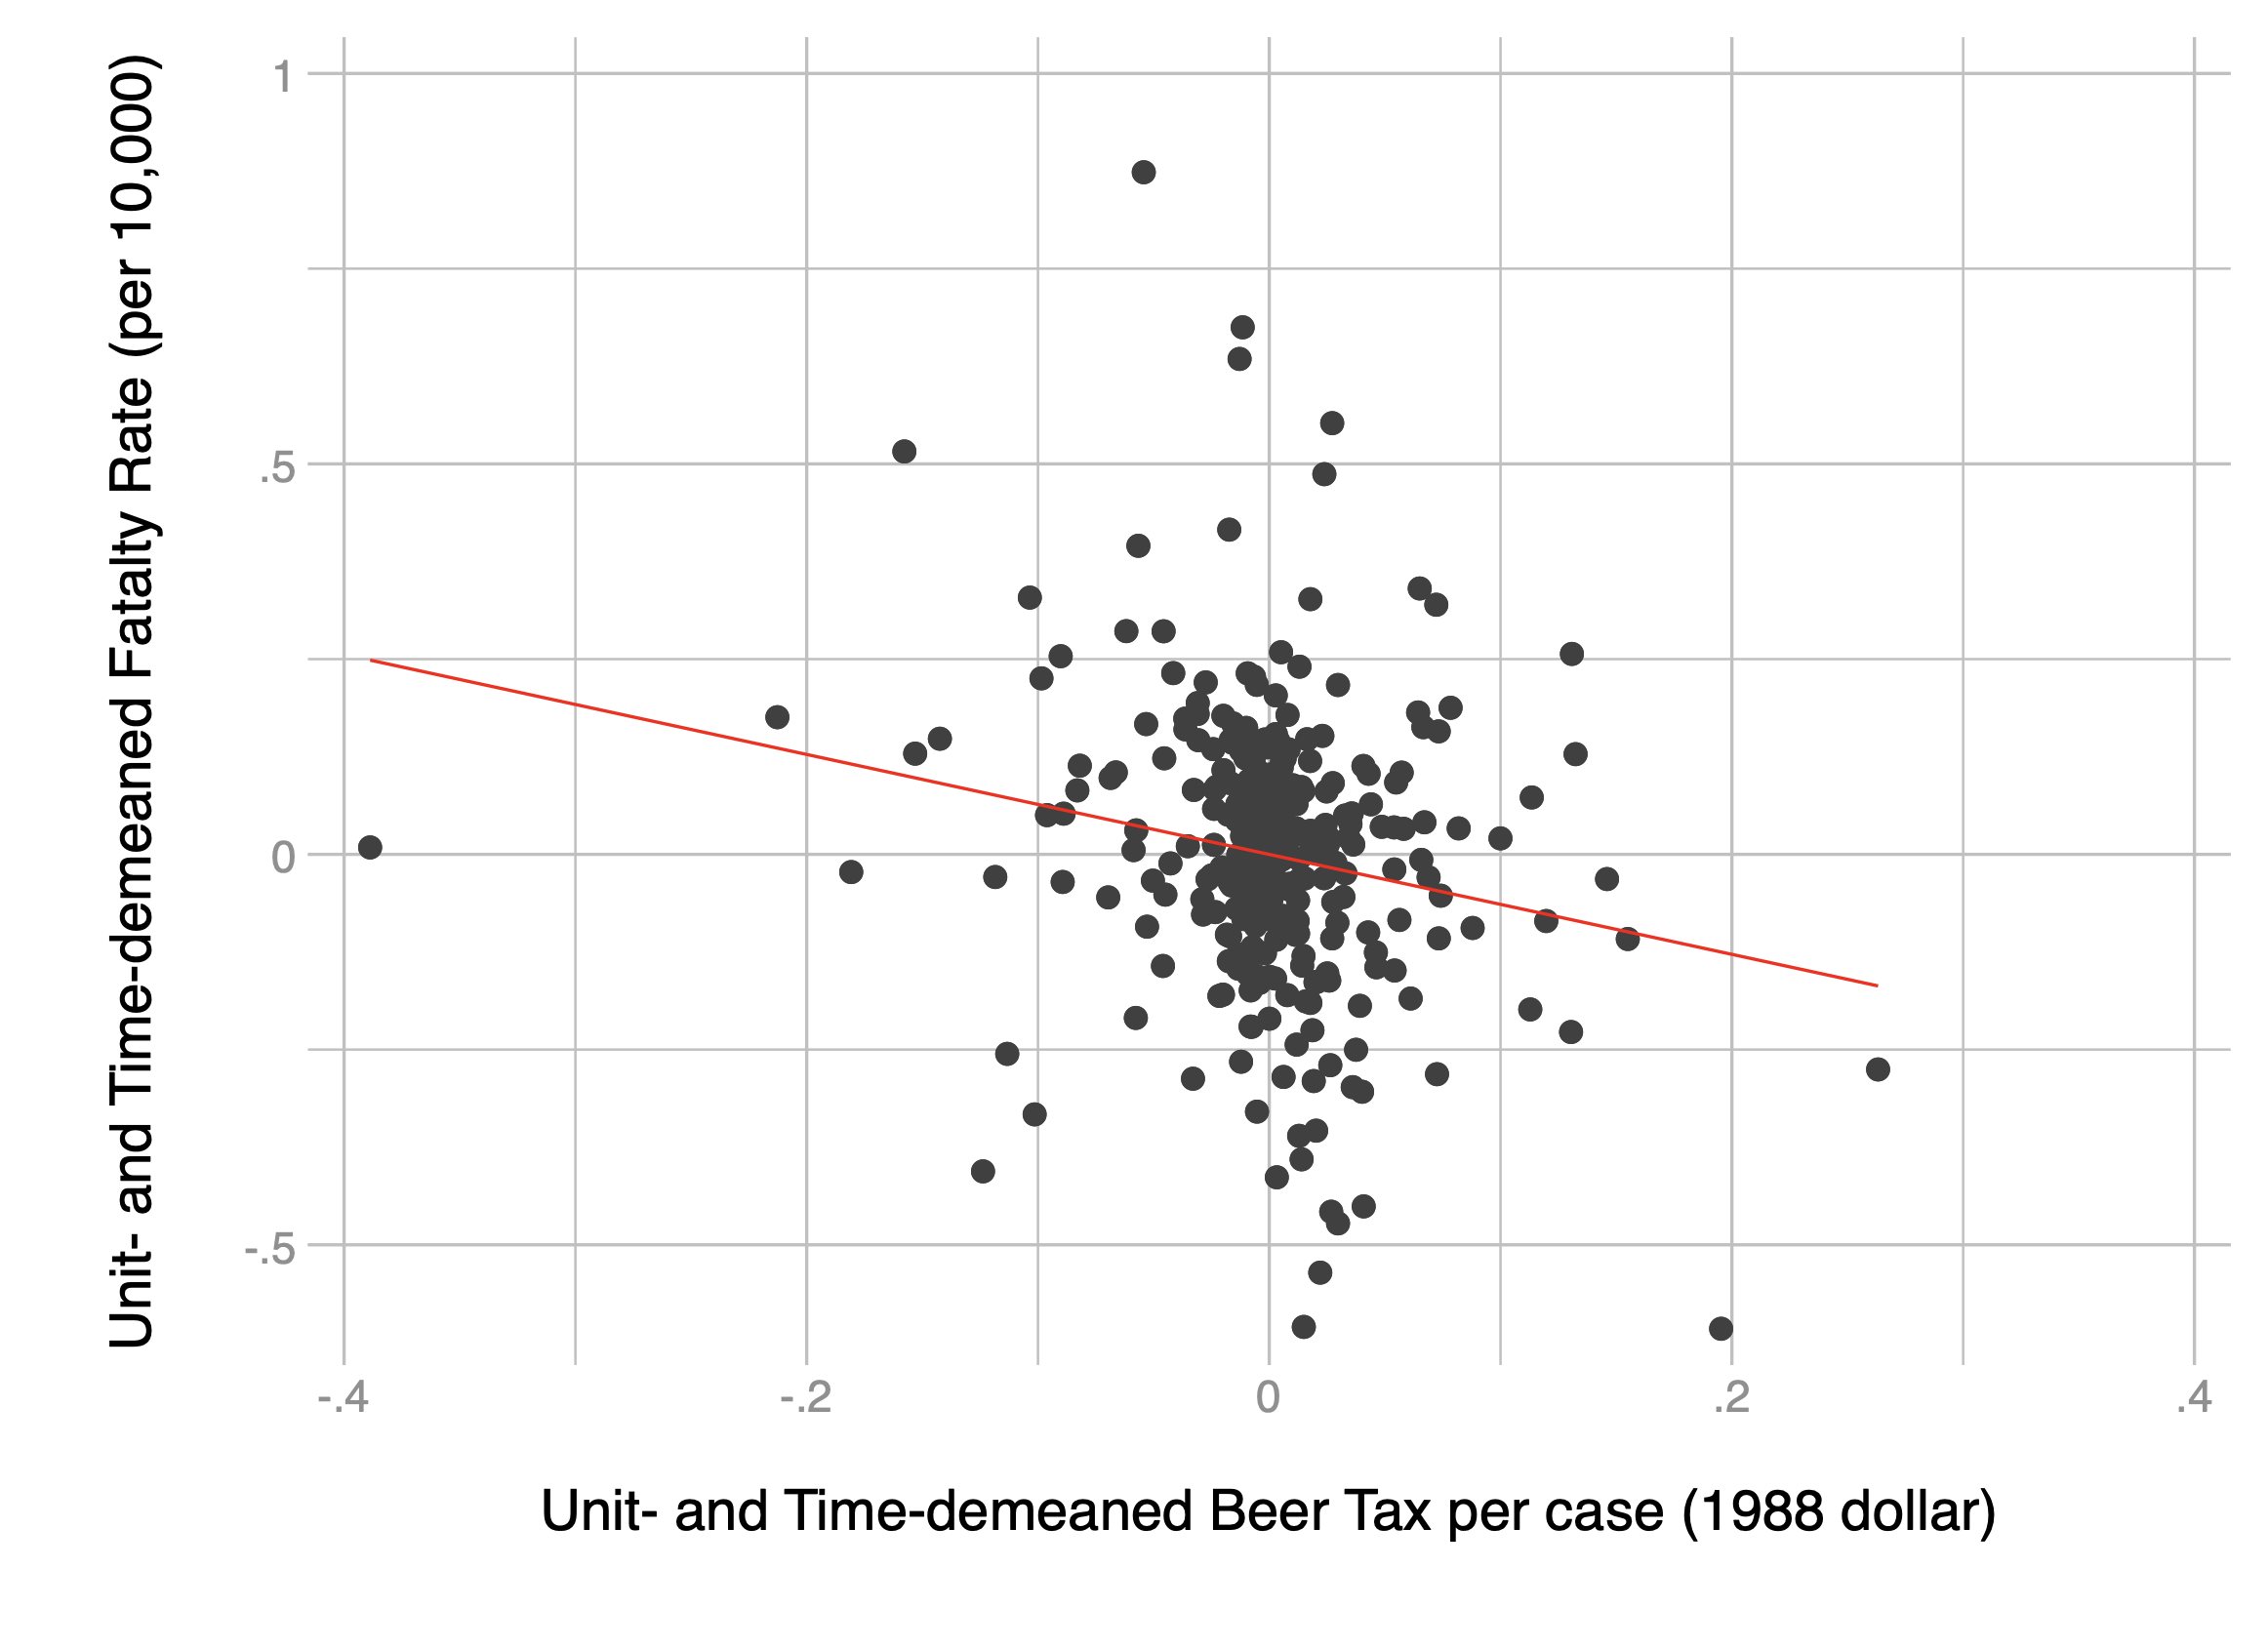
\includegraphics[width=.75\linewidth]{images/beertax_panel3.png}
\end{figure}
\end{frame}

\begin{frame}{Both unit and time fixed effects}
\begin{figure}
  \centering
         \vspace{-1mm}
         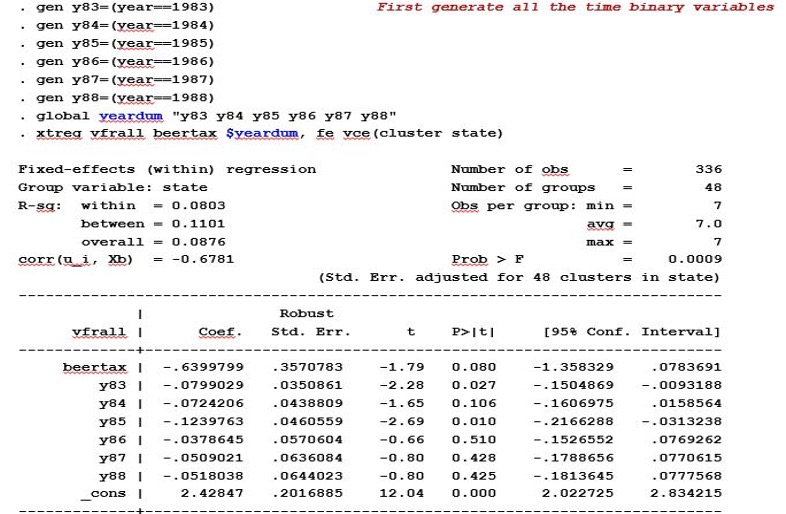
\includegraphics[width=.75\linewidth]{images/beertax_panel4.jpg}
\end{figure}
\end{frame}


\begin{frame}{The Fixed Effects Simple Regression Assumptions}
Consider the following regression model
\begin{equation*}
    Y_{it} = \alpha_i + \beta_1 X_{i,t} + u_{i,t}
\end{equation*}
\begin{enumerate}
    \item $\mathbb{E}(u_i\mid X_{i1}, X_{i2}, \dots, X_{iT}, \alpha_i, \lambda_t)=0$ 
    \item $(X_{i1}, X_{i2}, \dots, X_{iT}, u_{i1}, u_{i2}, \dots, u_{iT})$ are i.i.d. draws from their joint distribution
    \item Large outliers are unlikely: ($X_{it}, u_{i,t}$) have fourth moments.
    \item There is no perfect multicollinearity (multiple $X$'s)
\end{enumerate}\\[1em]

Assumption 1 means that the error term cannot be correlated with any present, past, or future value of $X$ (no omitted lagged effects, no feedback loop!)\\[1em]

Assumption 2 means that variables are independent across units but makes no such restriction within a unit.\\[1em]

Assumption 3 and 4 did not change (see Lecture 7).
\end{frame}

\begin{frame}{Serial Correlation}
 \begin{columns}
\begin{column}{0.35\textwidth}
\begin{itemize}
    \item Following up on Assumption 2, when $u_{i,t}$ is correlated over time within a unit, i.e., when $cov(u_{i,t}, u_{i,t+j})\neq 0$ we say that $u_{i,t}$ is \textbf{autocorrelated}, or \textbf{serially correlated}.\\
    \item If entities are sampled by simple random sampling, then $(u_{i1}, u_{i2}, \dots, u_{iT})$ is independent of $(u_{j1}, u_{j2}, \dots, u_{jT})$...
\end{itemize}
\end{column}
\begin{column}{0.7\textwidth}
\begin{figure}
  \centering
        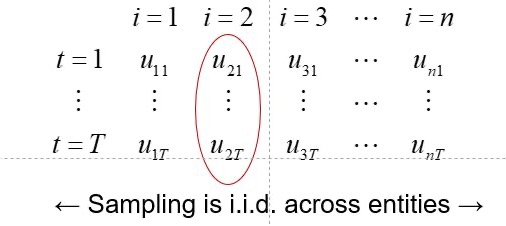
\includegraphics[scale=.5]{images/serial0.jpg}
\end{figure}
\begin{itemize}
    \item But in many panel data applications, $u_{i,t}$ is serially correlated
    \item[$\longrightarrow$] Clustering/Moulton's problem (1986)
\end{itemize}
\end{column}
\end{columns}
\end{frame}



\begin{frame}{Clustered SEs}
The usual OLS standard errors (both homoskedasticity-only and heteroskedasticity-robust) will in general be wrong because they assume that $u_{it}$ is serially uncorrelated.\\[1em]

In practice, they often understate the true sampling uncertainty: if $u_{it}$ are correlated over time, you don’t have as much information (as much random variation) as you would if $u_{it}$ were uncorrelated!\\[1em]

To see this, consider the panel the panel (time-)demeaned regression estimator
\begin{equation*}
    \hat{\beta}_1 = \frac{\sum_{i=1}^n\sum_{t=1}^T (X_{it}-\bar{X}_i)(Y_{it}-\bar{Y}_i)}{\sum_{i=1}^n\sum_{t=1}^T (X_{it}-\bar{X}_i)^2} = \frac{\sum_{i=1}^n\sum_{t=1}^T \tilde{X}_{it} \tilde{Y}_{it}}{\sum_{i=1}^n\sum_{t=1}^T  \tilde{X}_{it}^2} = \beta_1 +  \frac{\frac{1}{nT}\sum_{i=1}^n\sum_{t=1}^T \tilde{X}_{it} \tilde{u}_{it}}{\frac{1}{nT} \sum_{i=1}^n\sum_{t=1}^T  \tilde{X}_{it}^2}
\end{equation*}\\[1em]
This completely mirrors the basic OLS estimator equation!!!
\end{frame}

\begin{frame}{Clustered SEs}
Rearranging the terms,

    \begin{equation*}
        \sqrt{nT}(\hat{\beta}_1 - \beta_1)  = \frac{\sqrt{\frac{1}{n}}\sum_{i=1}^n \sqrt{\frac{1}{T}} \sum_{t=1}^T 
 \tilde{X}_{it} \tilde{u}_{it} }{\frac{1}{nT} \sum_{i=1}^n\sum_{t=1}^T  \tilde{X}_{it}^2}  = \frac{\sqrt{\frac{1}{n}}\sum_{i=1}^n \eta_i }{\hat{Q}_{\tilde{X}}}
    \end{equation*}

Because $\eta_i$ is i.i.d across units (by Assumption 2), of mean 0 (by Assumption 1), with finite variance (by Assumption 3), then (same reasoning as in Lecture 3!)

    \begin{equation*}
  \sqrt{nT}(\hat{\beta}_1 - \beta_1)  = \frac{\sqrt{\frac{1}{n}}\sum_{i=1}^n \eta_i }{\hat{Q}_{\tilde{X}}} \sim \mathcal{N}\Big(0, \frac{\sigma_\eta^2}{{Q}_{\tilde{X}}^2} \Big) \text{~~~~ as $n$ grows large}
    \end{equation*}

Now, note that

\begin{equation*}
    \sigma_\eta^2 = var\Bigg(\sqrt{\frac{1}{T}} \sum_{t=1}^T 
 \tilde{X}_{it} \tilde{u}_{it}\Bigg) = \frac{1}{T} var\Big(\sum_{t=1}^T 
 \tilde{X}_{it} \tilde{u}_{it}\Big) = \frac{1}{T} var\Big[\tilde{X}_{i1} \tilde{u}_{i1}+\dots+ \tilde{X}_{iT} \tilde{u}_{iT}\Big]
\end{equation*}
\end{frame}

\begin{frame}{Clustered SEs}
Remember that $var(X + Y) = var(X) + var(Y) + 2cov(X,Y)$... therefore
\begin{eqnarray*}
    &\sigma_\eta^2 = &\frac{1}{T} \Big[var(\tilde{X}_{i1} \tilde{u}_{i1})+\dots+ var(\tilde{X}_{iT} \tilde{u}_{iT}) +\\
    & &2cov(\tilde{X}_{i1} \tilde{u}_{i1}, \tilde{X}_{i2} \tilde{u}_{i2}) + \dots + 2cov(\tilde{X}_{i,T-1} \tilde{u}_{i,T-1}, \tilde{X}_{iT} \tilde{u}_{iT}) \Big]
\end{eqnarray*}
The heteroskedasticity-robust variance formula seen so far misses all the (auto)covariances in the final part the equation... If there is a serial correlation, the usual heteroskedasticity-robust variance estimator is inconsistent!\\[1em]

Clustered SEs for panel data are the logical extension of heteroskedastic (HR) SEs for cross-section. In cross-section regression, HR SEs are valid whether or not there is HR. In panel data regression, clustered SEs are valid whether or not there is HR and/or serial correlation.\\[1em]

To conclude, the HR-robust clustered SEs reads
\begin{equation*}
    SE(\hat{\beta}_1)=\sqrt{\frac{1}{nT}\frac{s_{\hat{\eta}}^2}{\hat{Q}_{\tilde{X}}^2}}
\end{equation*}

\end{frame}

\begin{frame}{Final Remarks on Clustered SEs}
We can cluster SEs by unit of observation (e.g., serial correlation within states), but also across units (e.g., regions above states) if we suspect potential correlation in observations within these higher-level clusters.\\[1em]

However, asymptotic inference (as $n$ grows large) supposes we have a large number of clusters...\\[1em]% since we are at least clustering SEs at the unit-level (e.g., states)

This is not always the case. When there are too few clusters and serial correlation, standard errors might be biased!\\[1em]

In the Traffic Fatalities vs. Beer Tax example, is 48 (states) a number of clusters that is large enough? What should be done when there are too few clusters? This is out of the scope of this (introductory) lecture!
\end{frame}


\begin{frame}[allowframebreaks]{Material}
\begin{itemize}
    \item[--] \textbf{Textbooks:}
    \begin{itemize}
        \item Introduction to Econometrics, 4th Edition, Global Edition, by Stock and Watson -- Chapters 10 - 13
        \item Introductory Econometrics, 5th Edition, A Modern Approach, by Jeff. Wooldridge -- Chapters 13-14.
        \item Causal Inference, The Mixtape, by Scott Cunningham -- Chapter 7
    \end{itemize}
    \item[--] \textbf{Papers:}
    \begin{itemize}
        \item Ashenfelter, O., \& Krueger, A. (1994). Estimates of the economic return to schooling from a new sample of twins. The American economic review, 1157-1173.
        \item Ashenfelter, O., \& Rouse, C. (1998). Income, schooling, and ability: Evidence from a new sample of identical twins. The Quarterly Journal of Economics, 113(1), 253-284.
        \item Bertrand, M., Duflo, E., \& Mullainathan, S. (2004). How much should we trust differences-in-differences estimates?. The Quarterly journal of economics, 119(1), 249-275.
        \item Tanaka, S. (2014). Does abolishing user fees lead to improved health status? Evidence from post-apartheid South Africa. American economic Journal: economic policy, 6(3), 282-312.
    \end{itemize}
\end{itemize}
\scriptsize{
\bibliographystyle{ecta}
\bibliography{base} 
}
\end{frame}



\end{document}